\documentclass[11pt,a4paper,fleqn]{scrartcl}
\usepackage{float}  % for [H] placement if needed
\usepackage{amsmath}
\usepackage{amssymb}
\usepackage{graphicx}
\usepackage{caption}
\usepackage{amsmath, amssymb, bm}

\begin{document}

\title{Generalizing GLV to Autotoxicity Model}
\author{
	\small{%
		\href{https://orcid.org/}{Sabrina Spigno}\(^{1, *}\),
		\href{https://orcid.org/}{}\(^1\)
		\href{}{}\(^{1, *}\)
	}
}
\date{2024/2025}
\maketitle  

\section{Explicit Autotoxin Dynamics (December 9, 2025)}
The model version 1 with explicit dynamics for species-specific autotoxicity reads:
\begin{equation}
\frac{dn_i}{dt} = n_i \left(1 - \rho a_i - \sum_{j \neq i} C_{j} n_j + \lambda \right), \label{eq:model1}
\end{equation}

\begin{equation}
\frac{da_i}{dt} = \beta n_i - \delta a_i, \label{eq:model2}
\end{equation}

The same equations but in log-scale:

\begin{equation}
\frac{dlog(n_i)}{dt} =  \left(1 - \rho a_i - \sum_{j \neq i} C_{j} n_j + \frac{\lambda}{n_i} \right), \label{eq:modellog1}
\end{equation}

\begin{equation}
\frac{dlog(a_i)}{dt} = \beta\frac{n_i}{a_i} - \delta , \label{eq:modellog2}
\end{equation}
\clearpage

\subsection{From single to community level dynamics Model Autotoxin 1}

\paragraph{Single species dynamics Model Autotoxin 1: S=1}
Increasing the diluition rate of the autotoxin lead the model to act as a gLV, because the autotoxicity does not accumulate.

\begin{figure}[h!]
    \centering
    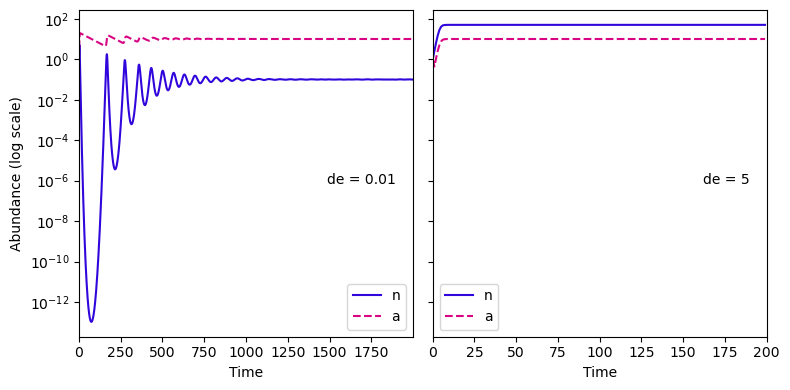
\includegraphics[width=\linewidth]{SingleSpecies/Model01species.png}
    \caption{Species (Purple) and Autotoxicity (Pink) dynamics in log space with $\delta$=0.01 on the left and $\delta$=5 on the right.}
\end{figure}
\label{simulationOneSpeciesModel0}


\clearpage
\paragraph{Two species dynamics Model Autotoxin 1: S=2}
Increasing the sensitivity to autotoxicity lead to the cohexistence of two species also if one species is more competitive of the other.

\begin{figure}[h!]
    \centering
    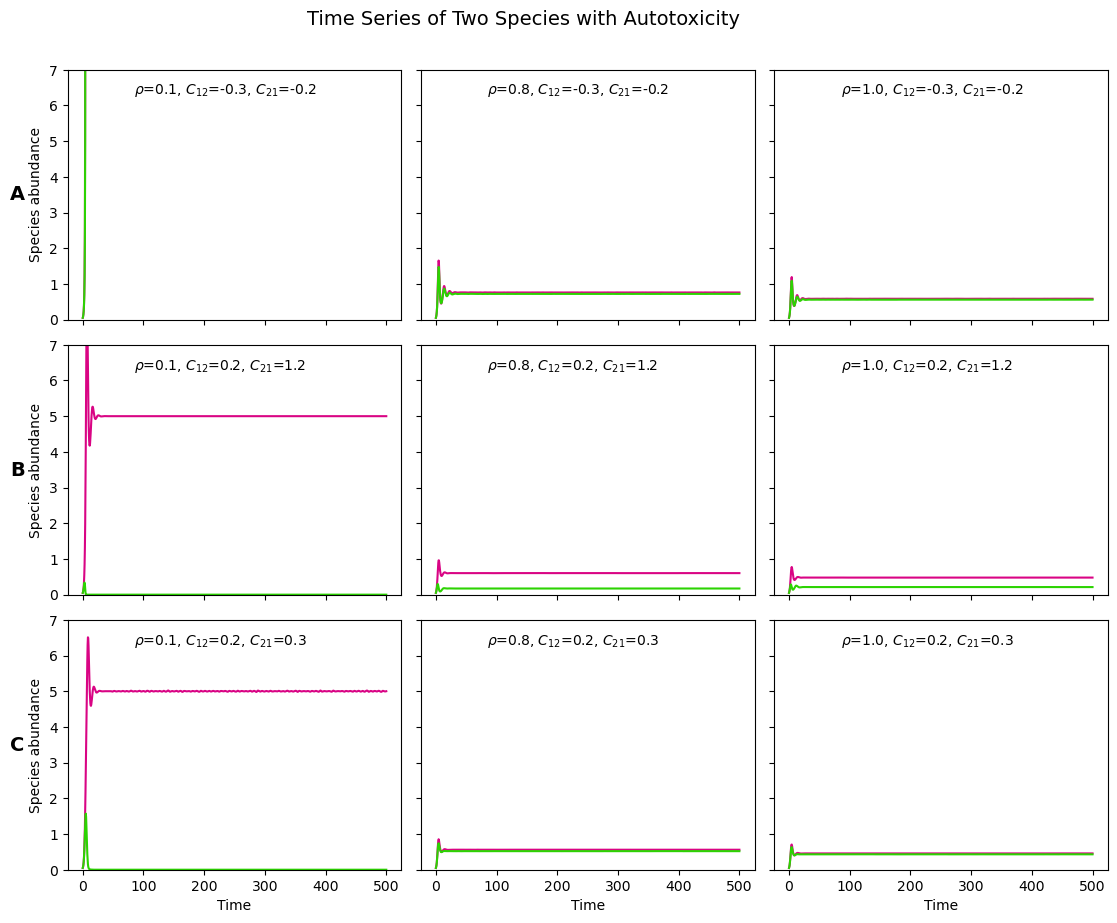
\includegraphics[width=\linewidth]{SingleSpecies/twospeciesModel0.png}
    \caption{Species (Purple) and Autotoxicity (Pink) dynamics in log space with $\delta$=0.01 on the left and $\delta$=5 on the right.}
\end{figure}
\label{simulationOneSpeciesModel0}



\section{GLV with Explicit Autotoxin Dynamics (February 12, 2025---  Onofrio Mazzarisi)}

The model version 1 with explicit dynamics for species-specific autotoxicity reads:
\begin{equation}
\frac{dn_i}{dt} = n_i \left(1 - \rho a_i - \sum_j C_{ij} n_j \right), \label{eq:model1again}
\end{equation}

\begin{equation}
\frac{da_i}{dt} = \beta n_i - \delta a_i, \label{eq:model2again}
\end{equation}

with $C_{ii} = 1$ for all $i$, and $\langle C_{ij} \rangle = \mu/S$, $\langle C_{ij} C_{kl} \rangle = \delta_{ik} \delta_{jl} \sigma^2 / S$.

An alternative setting is where $C_{ii} = 0$, attributing diagonal contributions solely to autotoxicity.

The corresponding GLV model for comparison is:

\begin{equation}
\frac{dn_i}{dt} = n_i \left(1 - \rho \frac{\beta}{\delta} n_i - \sum_j C_{ij} n_j \right), \label{eq:glv}
\end{equation}

using the same $C_{ij}$ statistics, optionally setting $C_{ii} = 0$.

In the limit of fast autotoxin dynamics relative to population dynamics, both models converge. The equilibrium values $n_i^*$ are the same in both:

Solving Eq.~\eqref{eq:model2} at stationarity:

\begin{equation}
a_i^* = \frac{\beta}{\delta} n_i^*, \label{eq:equilibrium_ai}
\end{equation}

which gives:

\begin{equation}
n_i^* = \frac{1 - \sum_{j \ne i} C_{ij} n_j^*}{1 + \rho \beta / \delta}, \label{eq:equilibrium_ni}
\end{equation}

To check feasibility, solve:

\begin{equation}
\sum_j \tilde{C}_{ij} n_j^* = 1, \label{eq:feasibility}
\end{equation}

with $\tilde{C}_{ij} = C_{ij}$ for $j \ne i$ and $\tilde{C}_{ii} = C_{ii} + \rho \beta / \delta$.

\subsection*{Jacobian Analysis}

Let $J$ be the Jacobian at equilibrium. For the GLV model:

\begin{equation}
J_{ij} = -C_{ij} n_i^*, \quad j \ne i,
\end{equation}
\begin{equation}
J_{ii} = -(1 + \rho \beta / \delta) n_i^*.
\end{equation}

For the model with explicit autotoxicity:

\[
J = 
\begin{bmatrix}
J_{nn} & J_{na} \\
J_{an} & J_{aa}
\end{bmatrix},
\]

with components:

\begin{align}
J_{nn, ij} &= -C_{ij} n_i^*, \quad i \ne j, \\
J_{nn, ii} &= -n_i^*, \\
J_{na, ij} &= 0, \\
J_{na, ii} &= -\rho n_i^*, \\
J_{an, ij} &= 0, \\
J_{an, ii} &= \beta, \\
J_{aa, ij} &= 0, \\
J_{aa, ii} &= -\delta.
\end{align}

The GLV Jacobian depends only on the combination:

\begin{equation}
\frac{\rho \beta}{\delta},
\end{equation}

while in the explicit model, $\rho$, $\beta$, and $\delta$ appear separately, potentially yielding distinct stability properties.

\section{Generalizing GLV to Autotoxicity Model (Emil Mallmin)}


Our starting point is the GLV:
\begin{equation}
\dot{n}_i = n_i\left( r_i - C_{ii} n_i - \sum_{j(\neq i)} C_{ij} n_j \right)
\end{equation}
This is a phenomenological and not a mechanistic model. The intra-specific suppression term, for instance, is meant to roughly capture the net effect of a variety of processes: conspecifics competition over resources, space, the effect of pathogens -- and autotoxicity. 

We should therefore think of the autotoxicity model as \emph{unpacking} some of the biological processes hidden in the phenomenological self-suppression term, rather than adding new mechanisms \emph{on top} of what's already represented by the GLV. This gives the generalization:
\begin{equation}
\dot{n}_i = n_i\left( r - C_{ii} h(n_i,a_i) - \sum_{j(\neq i)} C_{ij} n_j \right),
\end{equation}
with $a_i$ the autotoxin concentration. We want to preserve, in a sense, the interpretation of $C_{ii}$ as the net strength of self-suppression effects. The function $h(n,a)$ should partition these effects into a fraction $\gamma$ due to autotoxicity and the remaining fraction $1-\gamma$ due to the other implicit causes.

If we assume that individuals die due to autotoxicity at a rate proportional to the autotoxin concentration, then $h(n,a)$ is linear in both arguments. To have a notion of partitioning between $a$ and $n$, we must find what amount of $n$ constitutes an "equivalent" amount of $a$.

To this end, consider the autotoxicity dynamics. Production occurs at a per capita rate $\beta$ and degradation/dilution at a rate $\delta$:
\begin{equation}
\dot{a}_i = \beta n_i - \delta a_i.
\end{equation}
The formal solution is:
\begin{equation}
a_i(t) = \frac{\beta}{\delta} \int_{-\infty}^t K_\delta(t-s) n_i(s)\, ds
\end{equation}
where $K_\delta$ is an exponentially decaying memory kernel:
\begin{equation}
K_\delta(s) = \delta e^{-\delta|s|} \quad \Rightarrow \quad \int_{-\infty}^0 K_\delta(s)\, ds = 1
\end{equation}
We can therefore write:
\begin{equation}
a_i(t) = \frac{\beta}{\delta}\hat{n}_i(t)
\end{equation}b
where $\hat{n}_i$ is a historical weighted average of the abundance. The ratio $\beta/\delta$ is therefore the "conversion ratio" between suppression from autotoxicity and implicit density-dependent effects. The "unpacking" due to autotoxicity can be interpreted as:
\begin{equation}
C_{ii}n_i \rightarrow C_{ii}\left[ \gamma \hat{n}_i + (1-\gamma)n_i \right].
\end{equation}
Writing out the abundance dynamics in full:
\begin{equation}
\dot{n}_i = n_i\left[ r - C_{ii} \left(\gamma \frac{\delta}{\beta}a_i + (1-\gamma)n_i\right) - \sum_{j(\neq i)} C_{ij} n_j \right]
\end{equation}
There are \emph{three ways} that the autotoxicity model can exactly reduce to the GLV in this representation:
\begin{itemize}
  \item $\gamma \to 0$ (trivially)
  \item $\delta \to \infty$ (so that $\hat{n}_i \to n_i$)
  \item $\delta \to 0$ (but this is meaningless because autotoxicities explode)
\end{itemize}
For any values of $\gamma,\delta,\beta$, the fixed points are identical to those of the original GLV, although the stability properties can differ; the Jacobian of the autotoxicity model depends separately on these three parameters (compare Onofrio's notes).

\subsection{Comparison to Previous Parametrization}
Before we had written the model as:
\begin{equation}
\dot{n}_i / n_i = g ( 1 - \rho a_i ) - \sum_{j} B_{ij} n_j
\end{equation}
with the diagonal elements sometimes $B_{ii}=1$ other times $B_{ii}=0$, causing some confusion. Comparing the versions we have:
\begin{equation}
r=g, \quad C_{ii} \gamma \delta/\beta = g \rho, \quad C_{ii}(1-\gamma) = B_{ii}
\end{equation}

\subsection{Nondimensionalization}
To simplify the study of the model, we make use of the fact that the arbitrary choice of units to measure time, abundance, and autotoxicity concentration allow us to reduce the number of relevant parameters by three. A detailed analysis proceeds by substituting:
\begin{equation}
n = N\tilde{n}, \quad a = A\tilde{a}, \quad t= T\tilde{t}
\end{equation}
in the dynamics, where the tilde-variable is nondimensional and the capital letter is the units of measurement to be decided. This leads one to conclude that the natural choice is:
\begin{equation}
T = 1/r, \quad N= r/C_{ii}, \quad A=\beta/C_{ii}.
\end{equation}
Note that this only works if $C_{ii}$ does not depend on $i$, but this we assume. We similarly nondimensionalise the other parameters:
\begin{equation}
\beta = \tilde{\beta}A/TN, \quad \delta = \tilde{\delta}/T, \quad C_{ij} = \tilde{C}_{ij}TN.
\end{equation}
In practice, this procedure is equivalent to simply putting $r=1,\beta=1,C_{ii}=1$ and dropping all the tildes. Thus, the simplified model is:
\begin{align}
\label{eqnologspecies}
\dot{n}_i &= n_i\left[ 1 - \left(\gamma \delta a_i + (1-\gamma)n_i\right) - \sum_{j(\neq i)} C_{ij} n_j \right] + \lambda\\
\label{eqnologautotox}
\dot{a}_i &= n_i - \delta a_i
\end{align}
We draw $C_{ij}\sim \mathcal{N}(\mu,\sigma)$, i.e., not with weak interaction scaling. In the end there are (beside species richness $S$) four continuous parameters to study: $\mu,\sigma,\delta,\gamma$.

\subsection{Agenda}
To understand how the $(\mu,\sigma)$ phase diagram of the GLV (not assuming weak scaling) is extended in the $\delta,\gamma$ directions.
\begin{enumerate}
    \item First look at dynamics versus $\delta,\gamma$ for few pairs $(\mu,\sigma)$ lying in the different phases in the GLV case
    \item Assuming we then find a fixed $\delta$ for which $\gamma$ can change stability, do numerical bifurcation diagram in $\gamma$ to determine type. (Perhaps complement with Jacobian spectrum plots)
    \item For the GLV, an arc in $(\mu,\sigma)$-space with not-too-large radius $\mu_0$ and focal point $(1,0)$ will cross all the boundaries of non-diverging phases perpendicularly. With $\phi$ the angle of such an arc, look at the dynamics in the $(\phi,\gamma)$-plane for some fixed $\delta$, or in $(\phi,\delta)$-plane for $\gamma=1$.
\end{enumerate}

We move forward after getting a sense of the range of the dynamics from these studies.



\subsection{From single to community level results}
\date{May 2025}
\paragraph{Single species dynamics: S=1}

\begin{align}
\label{EqParametrizedSpecies}
\dot{n} &= n\left( 1 - \gamma \delta a - (1 - \gamma)n \right),\\
\label{EqParametrizedAutotoxicity}
\dot{a} &= n - \delta a,\\ \end{align},\\

We consider the system \ref{EqParametrizedSpecies} and \ref{EqParametrizedAutotoxicity}, and, at equilibrium, we set $\dot{n} = 0$ and $\dot{a} = 0$:
\[
n = \delta a \quad \Rightarrow \quad a = \frac{n}{\delta}
\]
Substitute into the first equation:
\[
\dot{n} = n \left( 1 - \gamma a n - (1 - \gamma) n \right) = n(1 - n)
\Rightarrow n^* = 1, \quad a^* = \frac{1}{\delta}
\]


\begin{figure}[H]
    \centering
    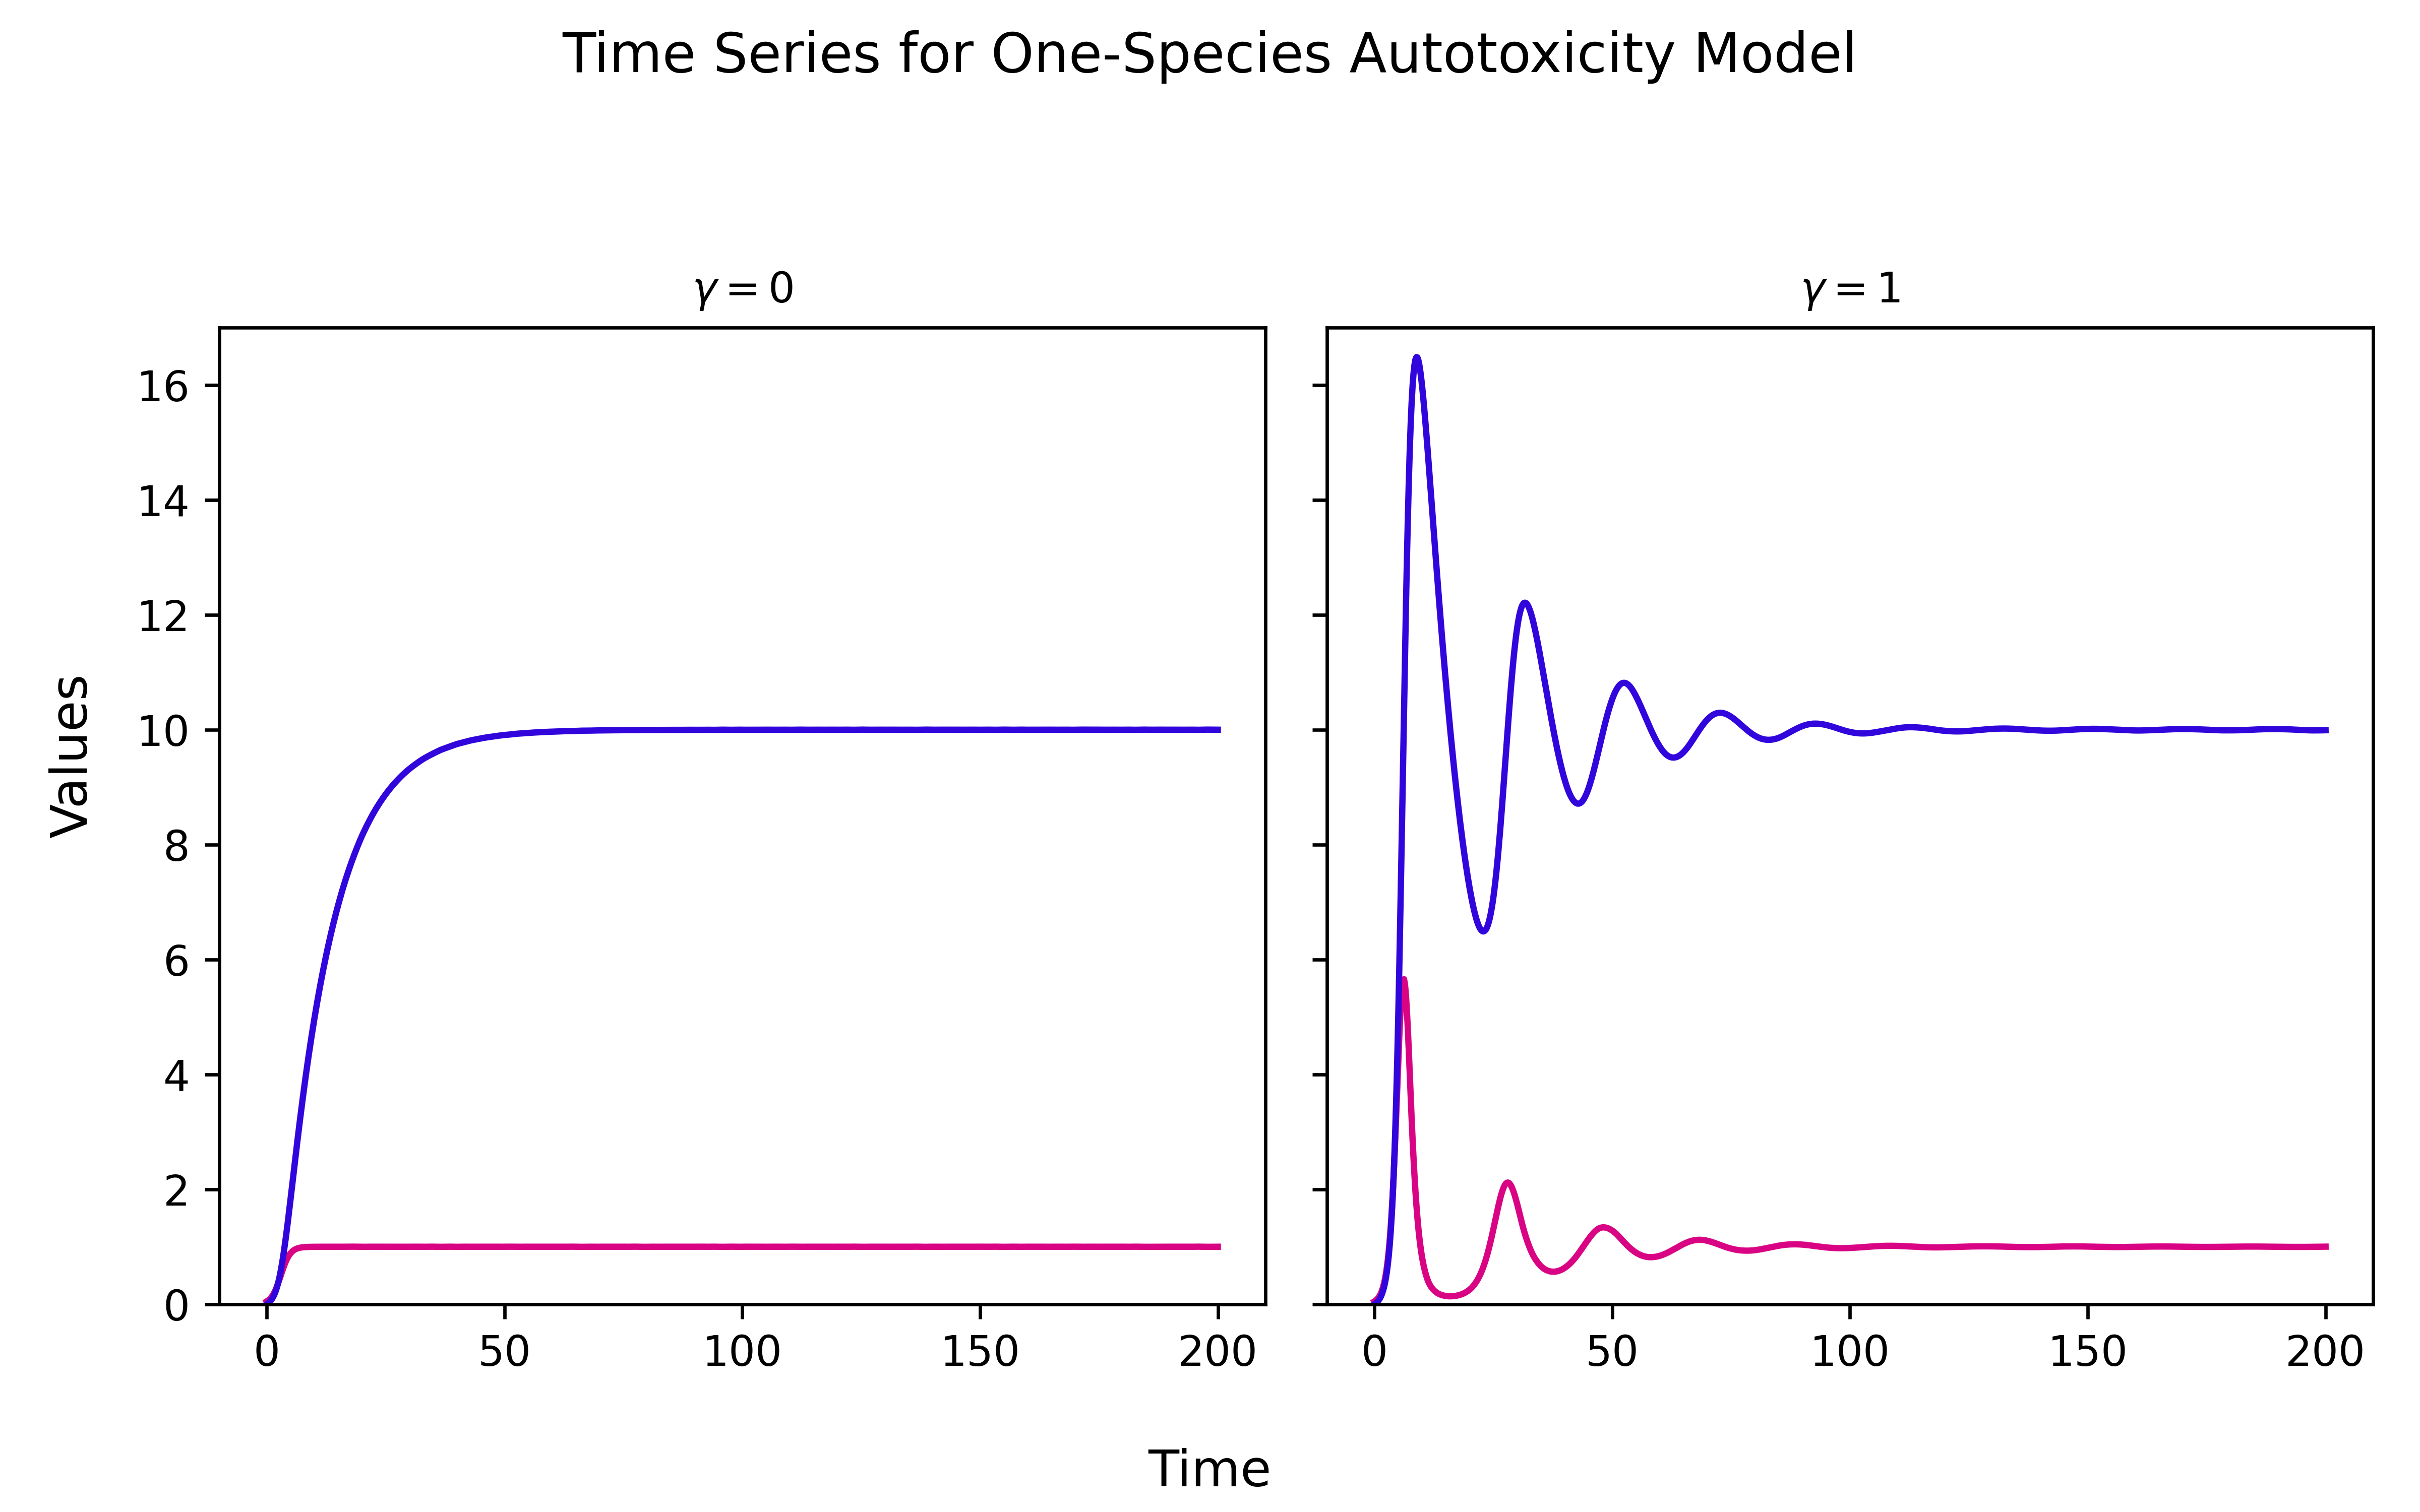
\includegraphics[width=\linewidth]{SingleSpecies/time_series_single_species.png}
    \caption{Species (Pink) and Autotoxicity (Purple) dynamics in Linear space with $\gamma$=0 on the left and $\gamma$=1 on the right.}
\end{figure}
\label{simulationOneSpecies}


The Jacobian $J$ for the equations \ref{EqParametrizedSpecies} and \ref{EqParametrizedAutotoxicity}:
\[
J = 
\begin{pmatrix}
J_{nn} & J_{na} \\
J_{an} & J_{aa}
\end{pmatrix}
\]

At the fixed point $(n^*, a^*) = (1, 1/\delta)$:
\begin{align*}
J_{nn} &= 1 - \gamma \delta a - 2(1 - \gamma)n = -1 + \gamma \\
J_{na} &= -\gamma \delta \\
J_{an} &= 1\\
J_{aa}&= -\delta\\
\end{align*}

\[
J =
\begin{pmatrix}
-1 + \gamma & -\gamma \delta \\
1 & -\delta
\end{pmatrix}
\]

The eigenvalues:
\[
\det(J - \lambda I) = 0
\]

\[
\begin{vmatrix}
-1 + \gamma - \lambda & -\gamma \delta \\
1 & -\delta - \lambda
\end{vmatrix}
= 0
\]

\[
(-1 + \gamma - \lambda)(-\delta - \lambda) + \gamma \delta = 0
\]

\[
(\lambda + 1 - \gamma)(\lambda + \delta) + \gamma \delta = 0
\]

\[
\lambda^2 + (1 - \gamma + \delta)\lambda + (1 - \gamma)\delta + \gamma \delta = 0
\]

\[
\lambda^2 + \left( (1 - \gamma) + \delta \right)\lambda + \delta = 0
\]

\[
\lambda = -\frac{(1 - \gamma) + \delta}{2} 
\pm 
\sqrt{\left( \frac{(1 - \gamma) + \delta}{2} \right)^2 - \delta}
\]

\begin{figure}[H]
    \centering
    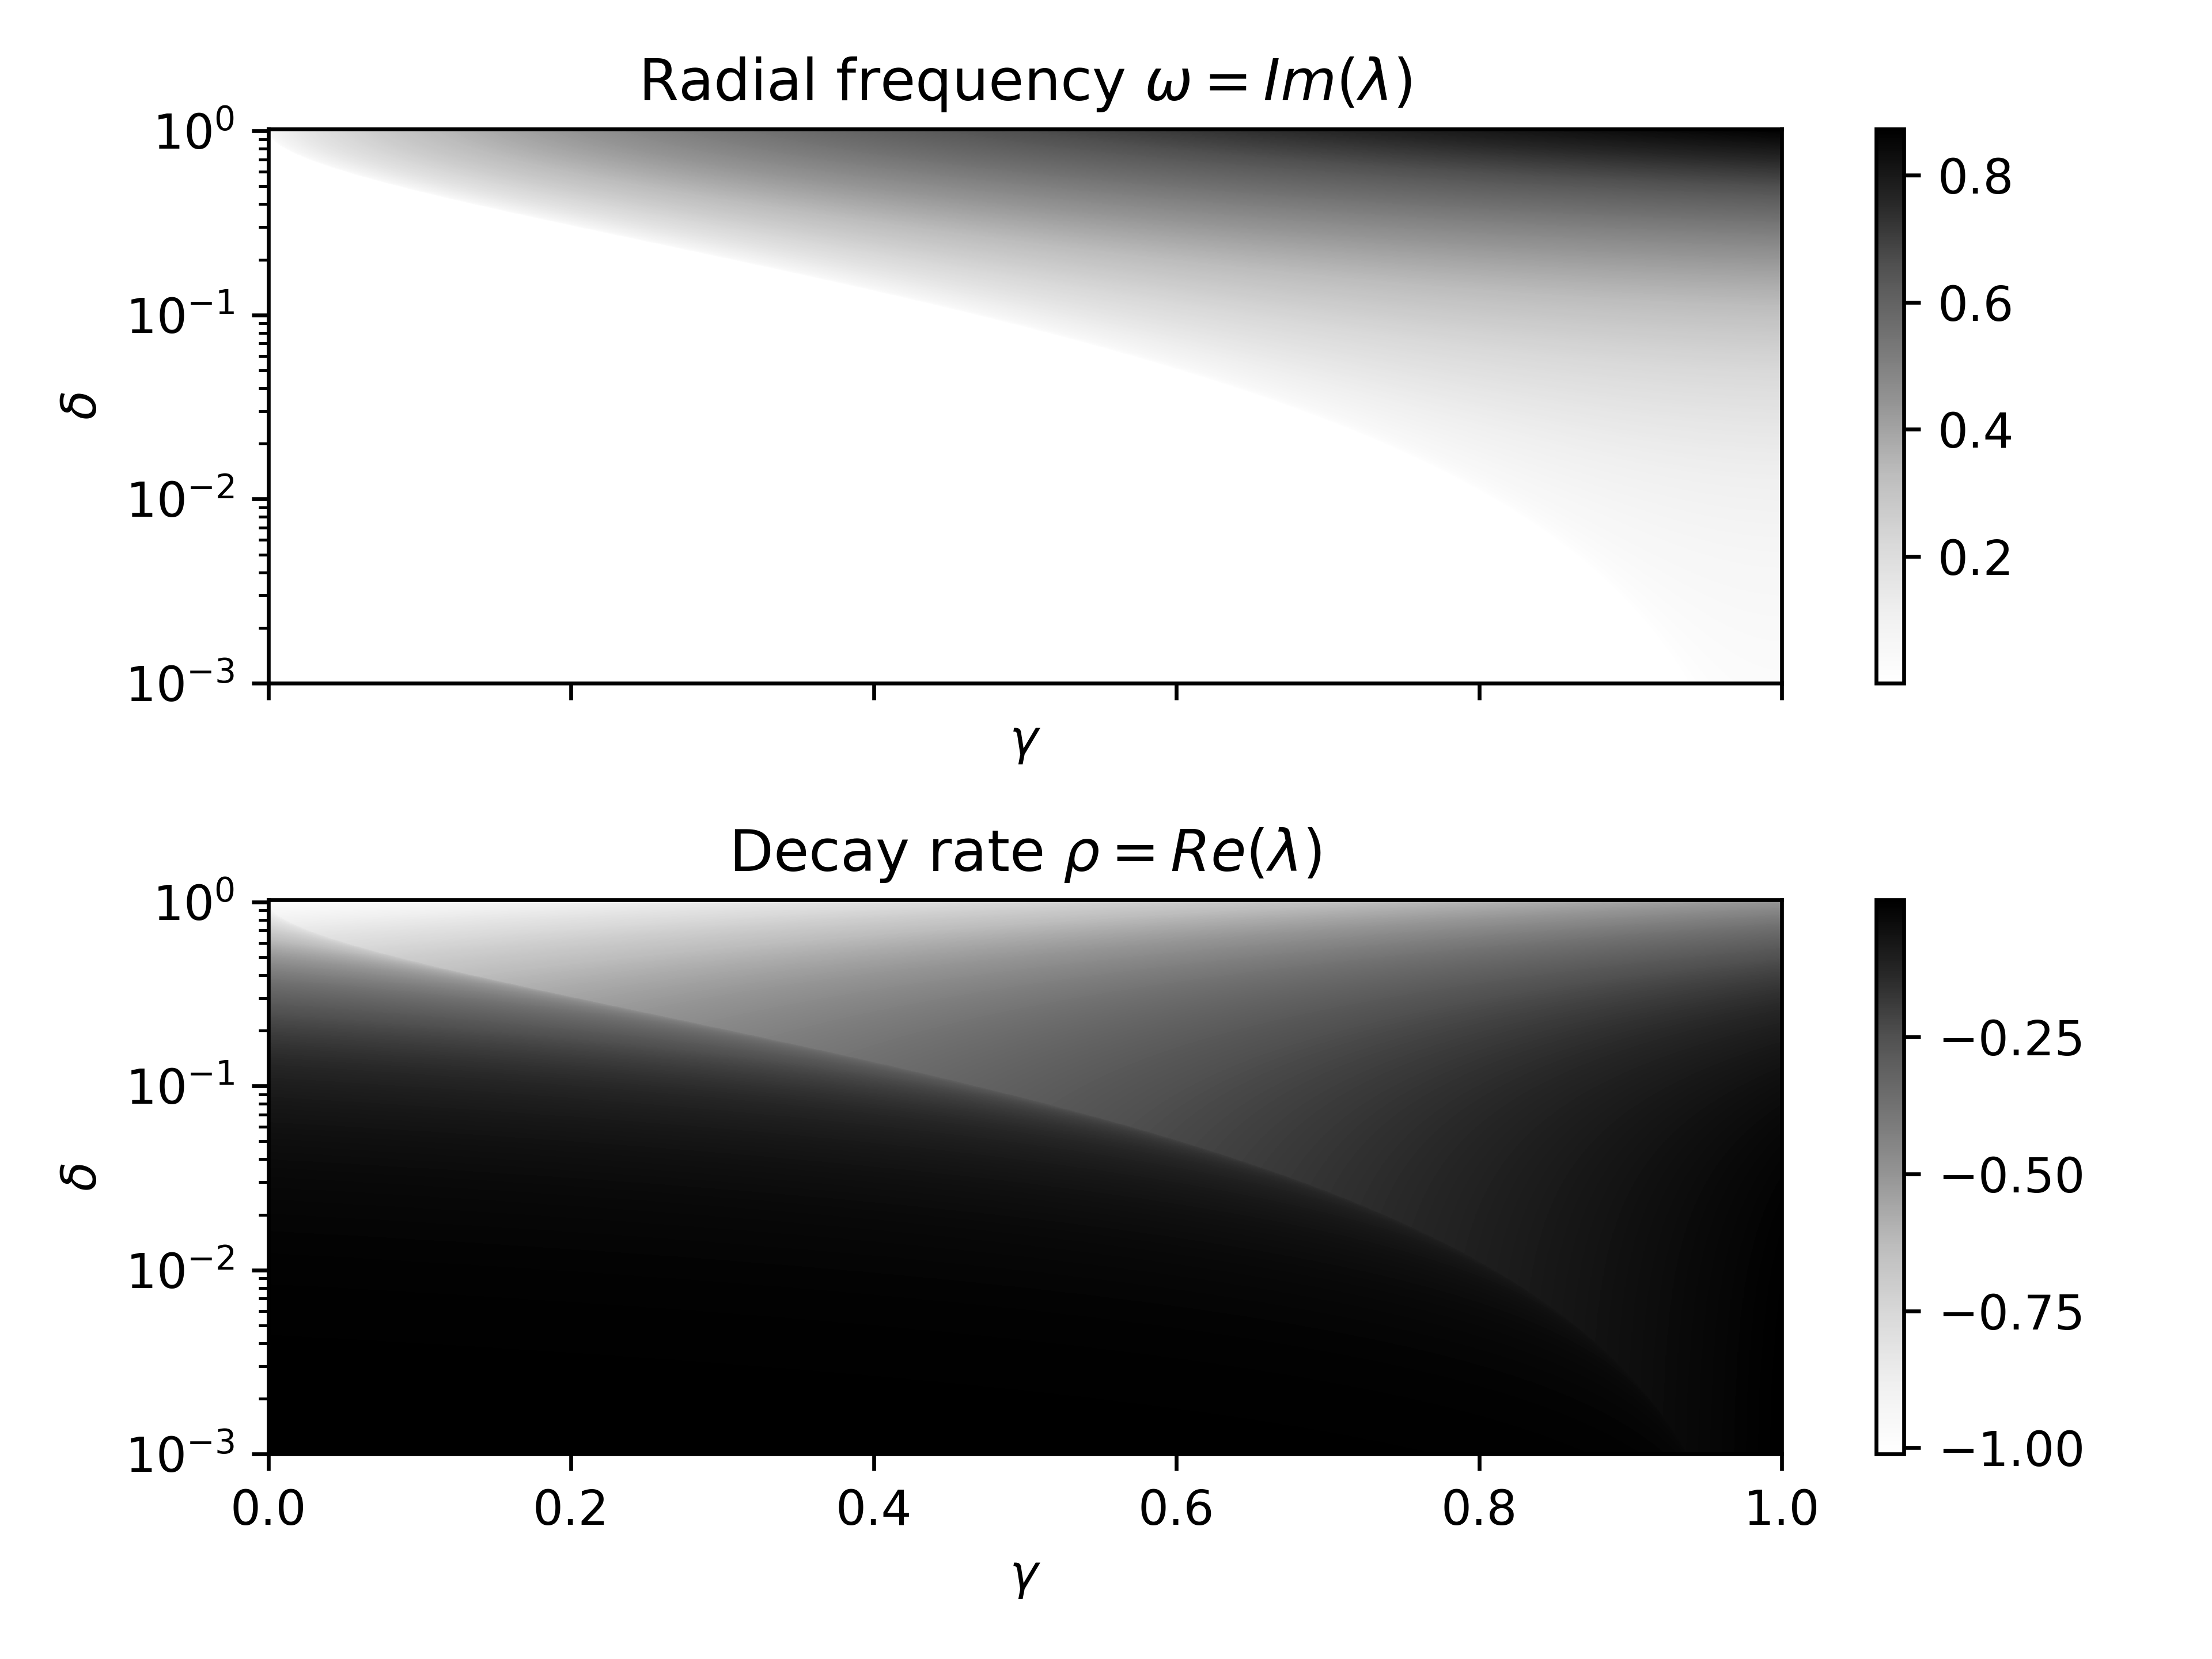
\includegraphics[width=\linewidth]{SingleSpecies/RadFreq.png}
    \caption{Imaginary and real parts of the eigenvalues as a function of $\gamma$ and $\delta$.}
\label{figRealandImaginaryPart}
\end{figure}

The heatmap of the eal and imaginary parts of the eigenvalues for different values of $\delta$ and $\gamma$ is showed in \ref{figRealandImaginaryPart}.
How to interpret:
\begin{itemize}
    \item The \textbf{real part} $\text{Re}(\lambda)$ determines the decay rate or growth.
        \begin{itemize}
            \item If $\text{Re}(\lambda) < 0$, the system decays to equilibrium (stable).
            \item If $\text{Re}(\lambda) > 0$, the system is unstable.
        \end{itemize}
    \item The \textbf{radial frequency} $\omega = \text{Im}(\lambda)$ determines the frequency of oscillation.
        \begin{itemize}
            \item If $\omega = 0$, no oscillation.
            \item If $0 < \omega < 1$, the oscillations are slow.
        \end{itemize}
In the current system, the decay rate is always negative, meaning the system is stable. The radial frequency remains below 1, indicating slow oscillations. Taken together, this implies that the system exhibits damped oscillations. It is visible also from the simulations in \ref{simulationOneSpecies}.
\end{itemize}


\paragraph{Two Species Dynamics: $S=2$}

\begin{align}
\dot{n}_1 &= n_1 \left[ 1 - \left( \gamma \delta a_1 + (1 - \gamma) n_1 \right) - C_{12} n_2(t) \right] \tag{Species 1} \\
\dot{n}_2 &= n_2\left[ 1 - \left( \gamma \delta a_2 + (1 - \gamma) n_2 \right) - C_{21} n_1(t) \right] \tag{Species 2} \\
\dot{a}_1 &= n_1 - \delta a_1(t) \tag{Autotoxin 1} \\
\dot{a}_2 &= n_2 - \delta a_2(t) \tag{Autotoxin 2}
\end{align}

\begin{figure}[H]
    \centering

    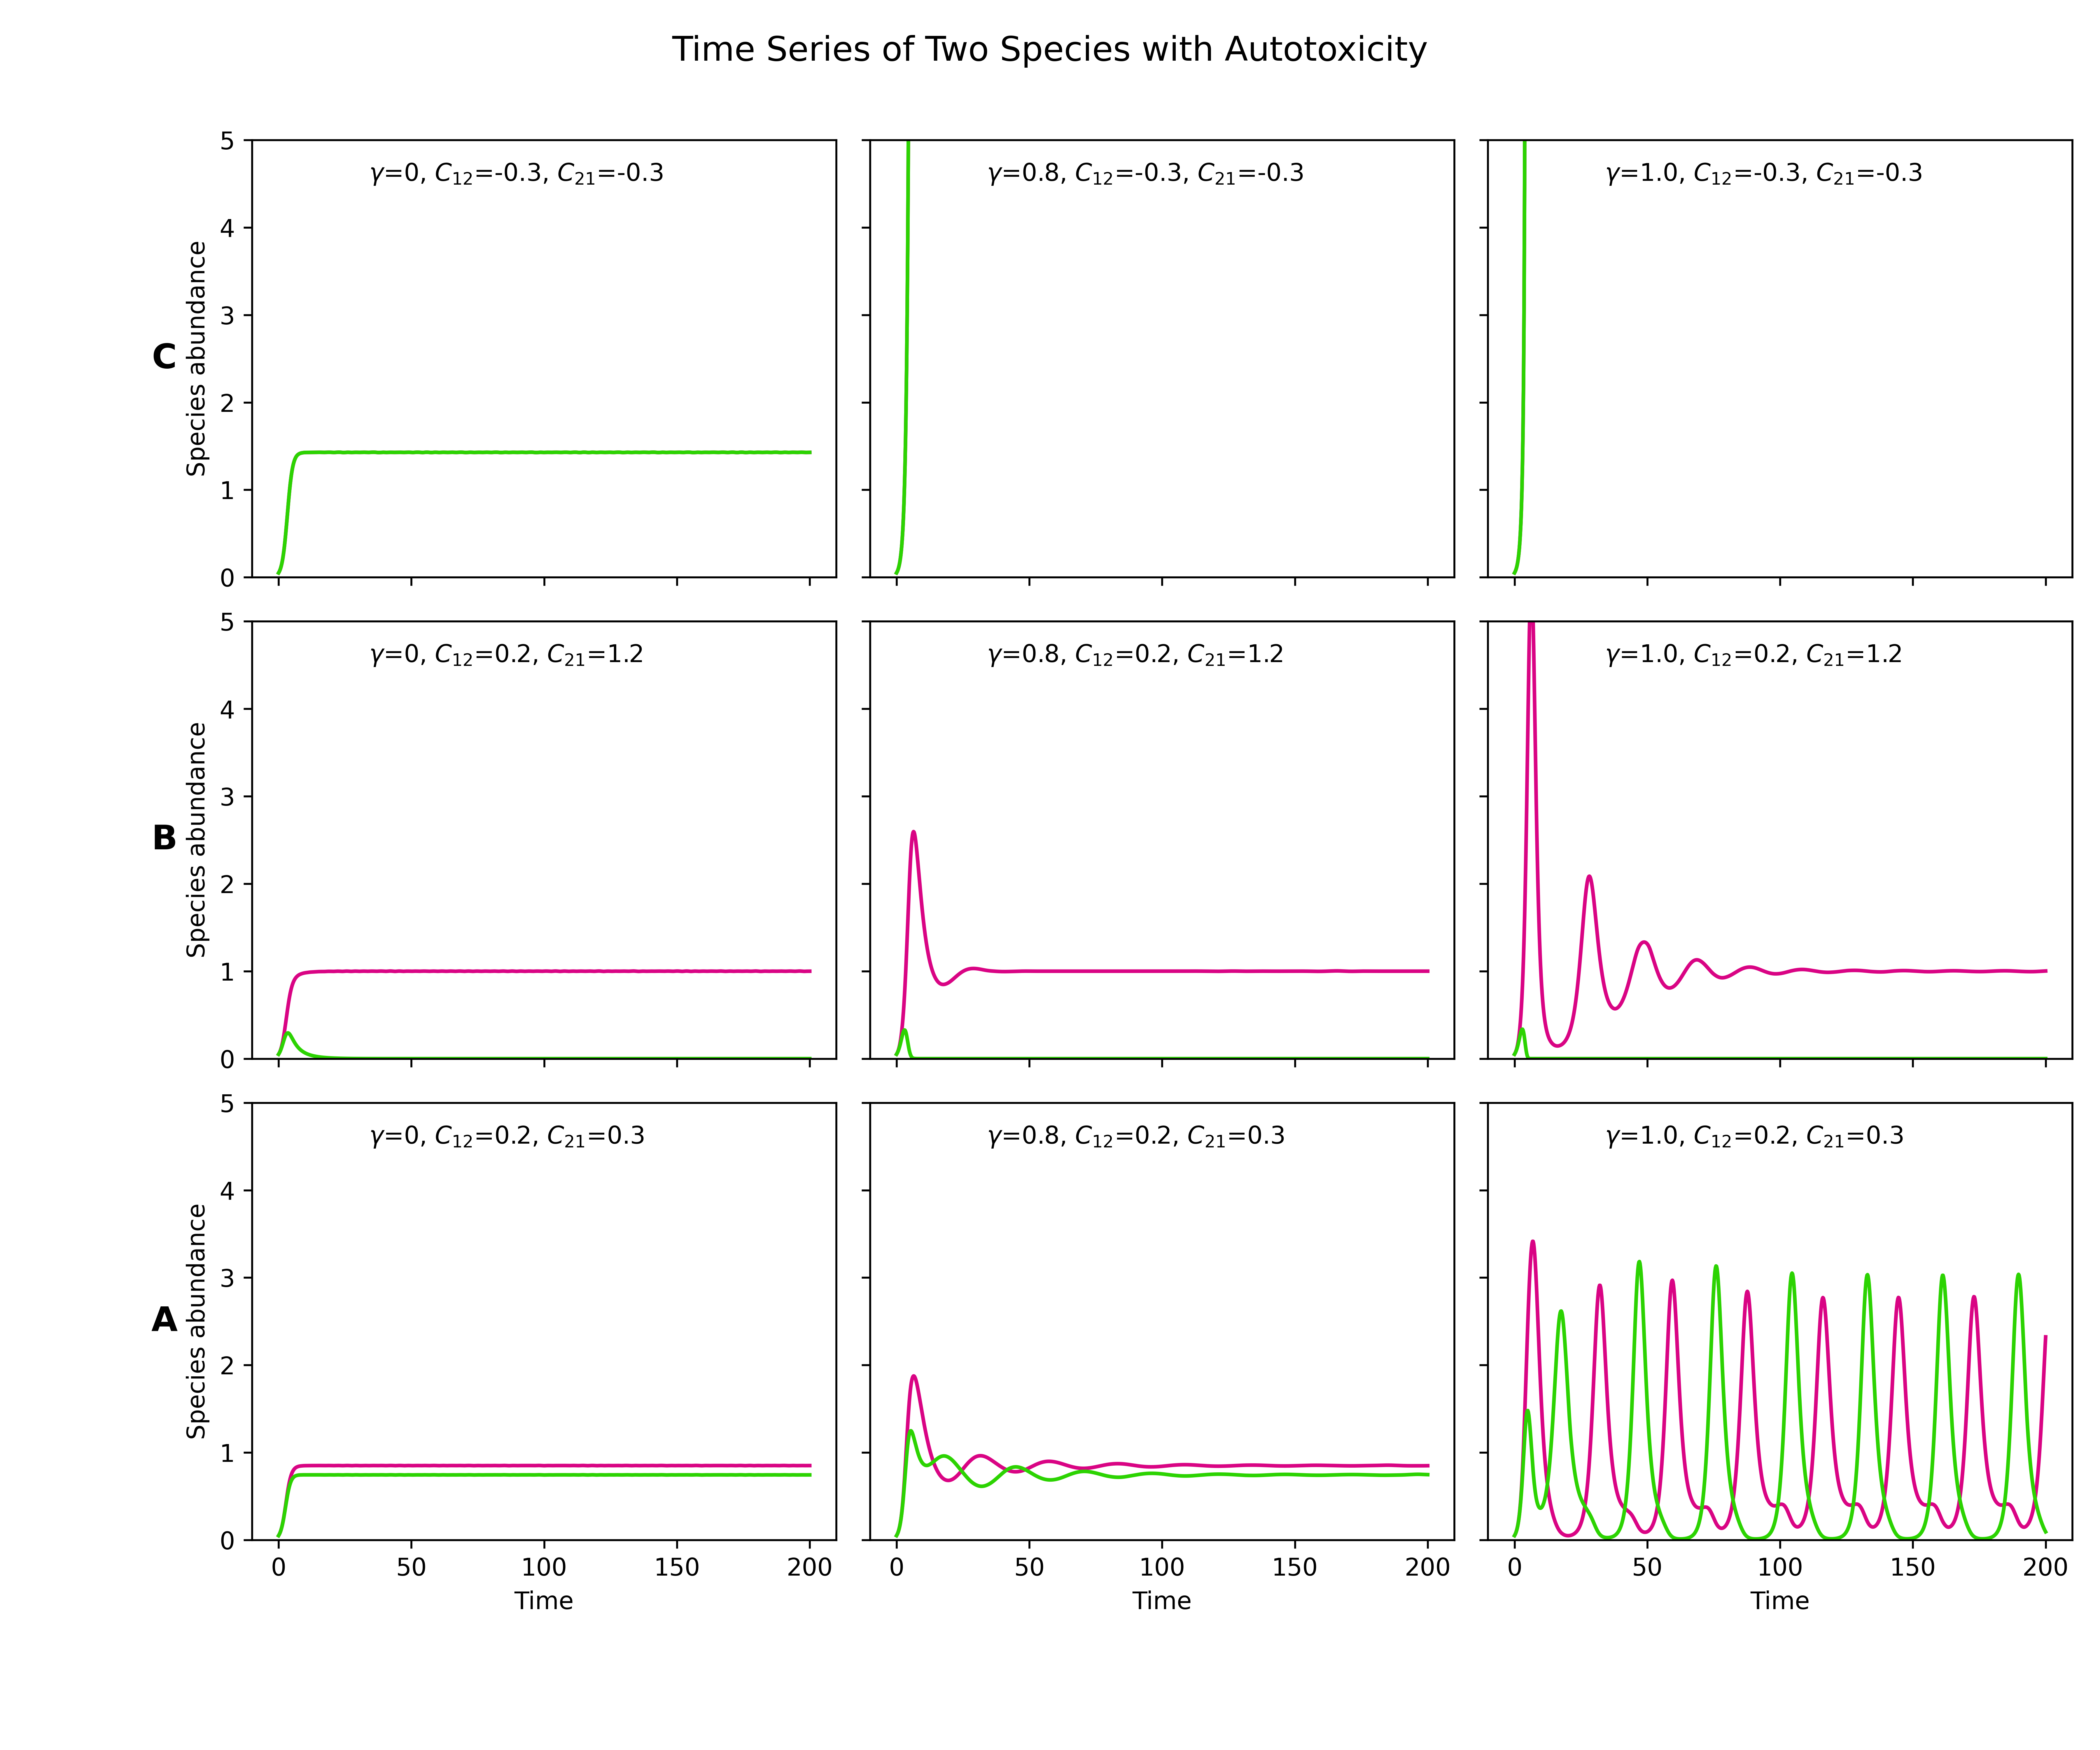
\includegraphics[width=\linewidth]{SingleSpecies/TwoSpecies3Cases.png}
    \caption{Species 1 (green) and Species 2 (pink) dynamics in linear space with $\gamma=0$, $\gamma=0.8$, and $\gamma=1$. The interaction between the two species varies from top to bottom. 
    (A) Both species positively influence each other with equal interaction strengths. 
    (B) The species compete, and Species 2 exerts a stronger negative influence on Species 1. 
    (C) The species compete, with Species 2 having a slightly higher competition parameter.}
\label{figtwospecies}
\end{figure}

The dynamics of two species is showed in Figure~\ref{figtwospecies}, with 3 different values of $\gamma$ and 3 different combinations of $C_{12}$ and $C_{21}$.
When $C_{12}$ and $C_{21}$ are both negative (meaning that they cooperate) --first row of the panel--, the increasing of autotoxicity-- from the left to the side-- lead the system to explode. Looking at the second row of the panel, when the species compete, -- and species 2 has an higher competitive parameter $C_{21}$=1.2, the species will not cohexist and the increasing of autotoxicity will lead to the same result of the gLV. When the specie compete to each other with lower parameters of competition, increasing autotoxicity will lead to an "oscillatory" cohexistence between the two species. 



\paragraph{Community dynamics: S=500}
We consider the system of equations \ref{eqnologspecies} and \ref{eqnologautotox} and also the same system but in a log-transformed space of $S$ interacting species with autotoxicity.
The system in log space is governed by the equations:
\begin{align}
\label{eqlogcommunitydynamicsspecies}
\frac{d}{dt} \log n_i &= 1 - \left( \gamma \delta a_i + (1 - \gamma) n_i \right) - \sum_{j \ne i} C_{ij} n_j + \frac{\lambda}{n_i} \\
\label{eqlogcommunitydynamicsautotoxicity}
\frac{d}{dt} \log a_i &= \frac{n_i}{a_i} - \delta
\end{align}

with $n_i = e^{\log n_i}$ and $a_i = e^{\log a_i}$.

We consider the log-transformed system of $S$ interacting species with autotoxicity, with the equations \ref{eqlogcommunitydynamicsspecies} and \ref{eqlogcommunitydynamicsautotoxicity}:
At equilibrium:

\[
\begin{aligned}
1 - \gamma \delta a_i - (1 - \gamma) n_i - \sum_{j \ne i} C_{ij} n_j + \frac{\lambda}{n_i} &= 0, \\
\frac{n_i}{a_i} - \delta &= 0, \\
\text{Substitute into the first equation: } 
a_i &= \frac{n_i}{\delta}\\
1 - \gamma \delta \cdot \frac{n_i}{\delta} - (1 - \gamma) n_i - \sum_{j \ne i} C_{ij} n_j + \frac{\lambda}{n_i} &= 0, \text{that lead to}
- \sum_{j \ne i} C_{ij} n_j + \frac{\lambda}{n_i} &= 0 \\
\end{aligned}
\]
The equilibrium does depend on the interacting matrix but does not depend on $\gamma$ and $\delta$.\\
Then, we define the Jacobian as:
\[
J =
\begin{bmatrix}
J_{nn} & J_{na} \\
J_{an} & J_{aa}
\end{bmatrix},
\]
In the linear space:

\[
J_{nn} =
\begin{cases}
- C_{ij} \cdot n_j & \text{if } i \ne j, \\
1 - \gamma \delta a_i - 2(1-\gamma) n_i - \sum_{j \ne i} C_{ij} n_j \sum \lambda n_i & \text{if } i = j.
\end{cases}
\]

\[
J_{na} =
\begin{cases}
- \gamma \delta n_i & \text{if } i = j, \\
0 & \text{otherwise}.
\end{cases}
\]

\[
J_{an} =
\begin{cases}
1 & \text{if } i = j, \\
0 & \text{otherwise}.
\end{cases}
\]

\[
J_{aa} =
\begin{cases}
-\delta & \text{if } i = j, \\
0 & \text{otherwise}.
\end{cases}
\]

\clearpage
In log space:

\[
J_{nn} =
\begin{cases}
- C_{ij} \cdot n_j & \text{if } i \ne j, \\
- (1 - \gamma) n_i - \dfrac{\lambda}{n_i} & \text{if } i = j.
\end{cases}
\]

\[
J_{na} =
\begin{cases}
- \gamma \delta a_i & \text{if } i = j, \\
0 & \text{otherwise}.
\end{cases}
\]

\[
J_{an} =
\begin{cases}
\dfrac{n_i}{a_i} & \text{if } i = j, \\
0 & \text{otherwise}.
\end{cases}
\]

\[
J_{aa} =
\begin{cases}
- \dfrac{n_i}{a_i} & \text{if } i = j, \\
0 & \text{otherwise}.
\end{cases}
\]


\clearpage

\paragraph{Simulations changing $\sigma$ $\gamma$}
\[
C_{ij} \sim \mathcal{N}(\mu, \sigma), \quad 
\mu = 0.2,\quad \sigma \in [0.001, 0.1], \quad 
\gamma \in [0, 1], \quad \delta = 0.01, \quad \lambda = 10^{-8}
\]

\begin{figure}[H]
    \centering
    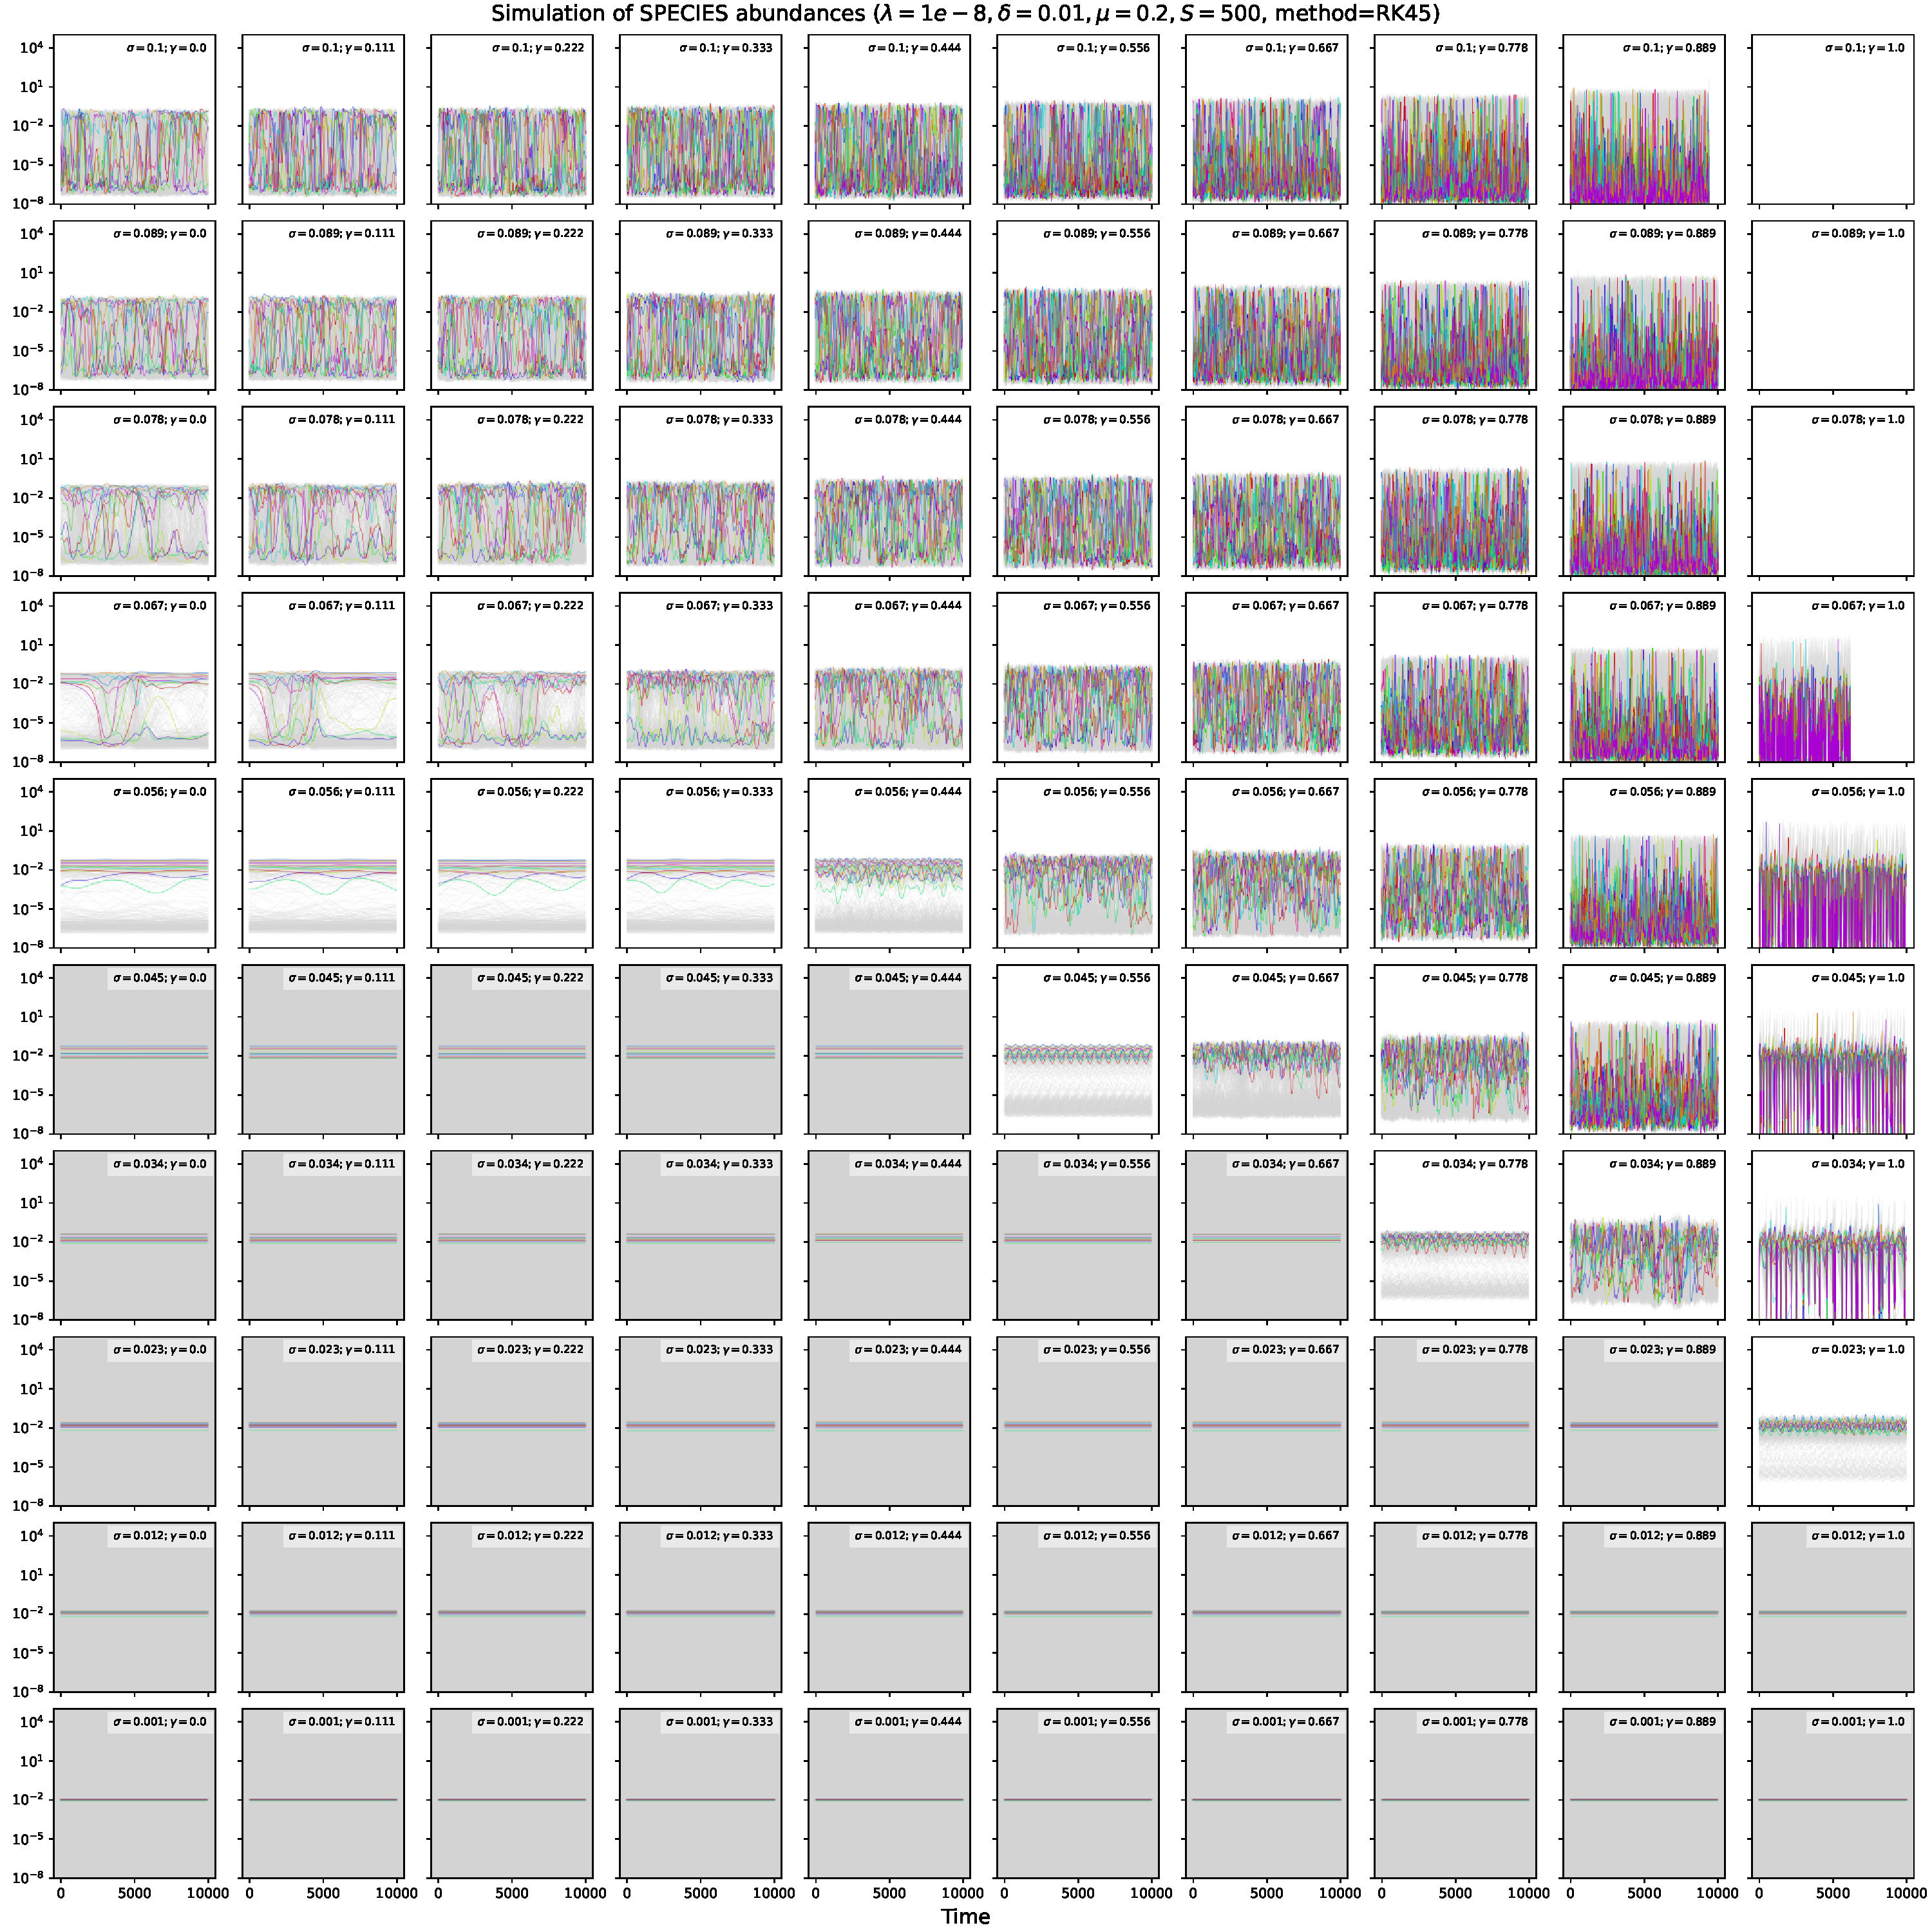
\includegraphics[width=\linewidth]{SigmaGamma/10Species.pdf}
    \caption{Species dynamics in logarithmic scale $\sigma$ and $\gamma$.}
\end{figure}

\clearpage

\begin{figure}[H]
    \centering
    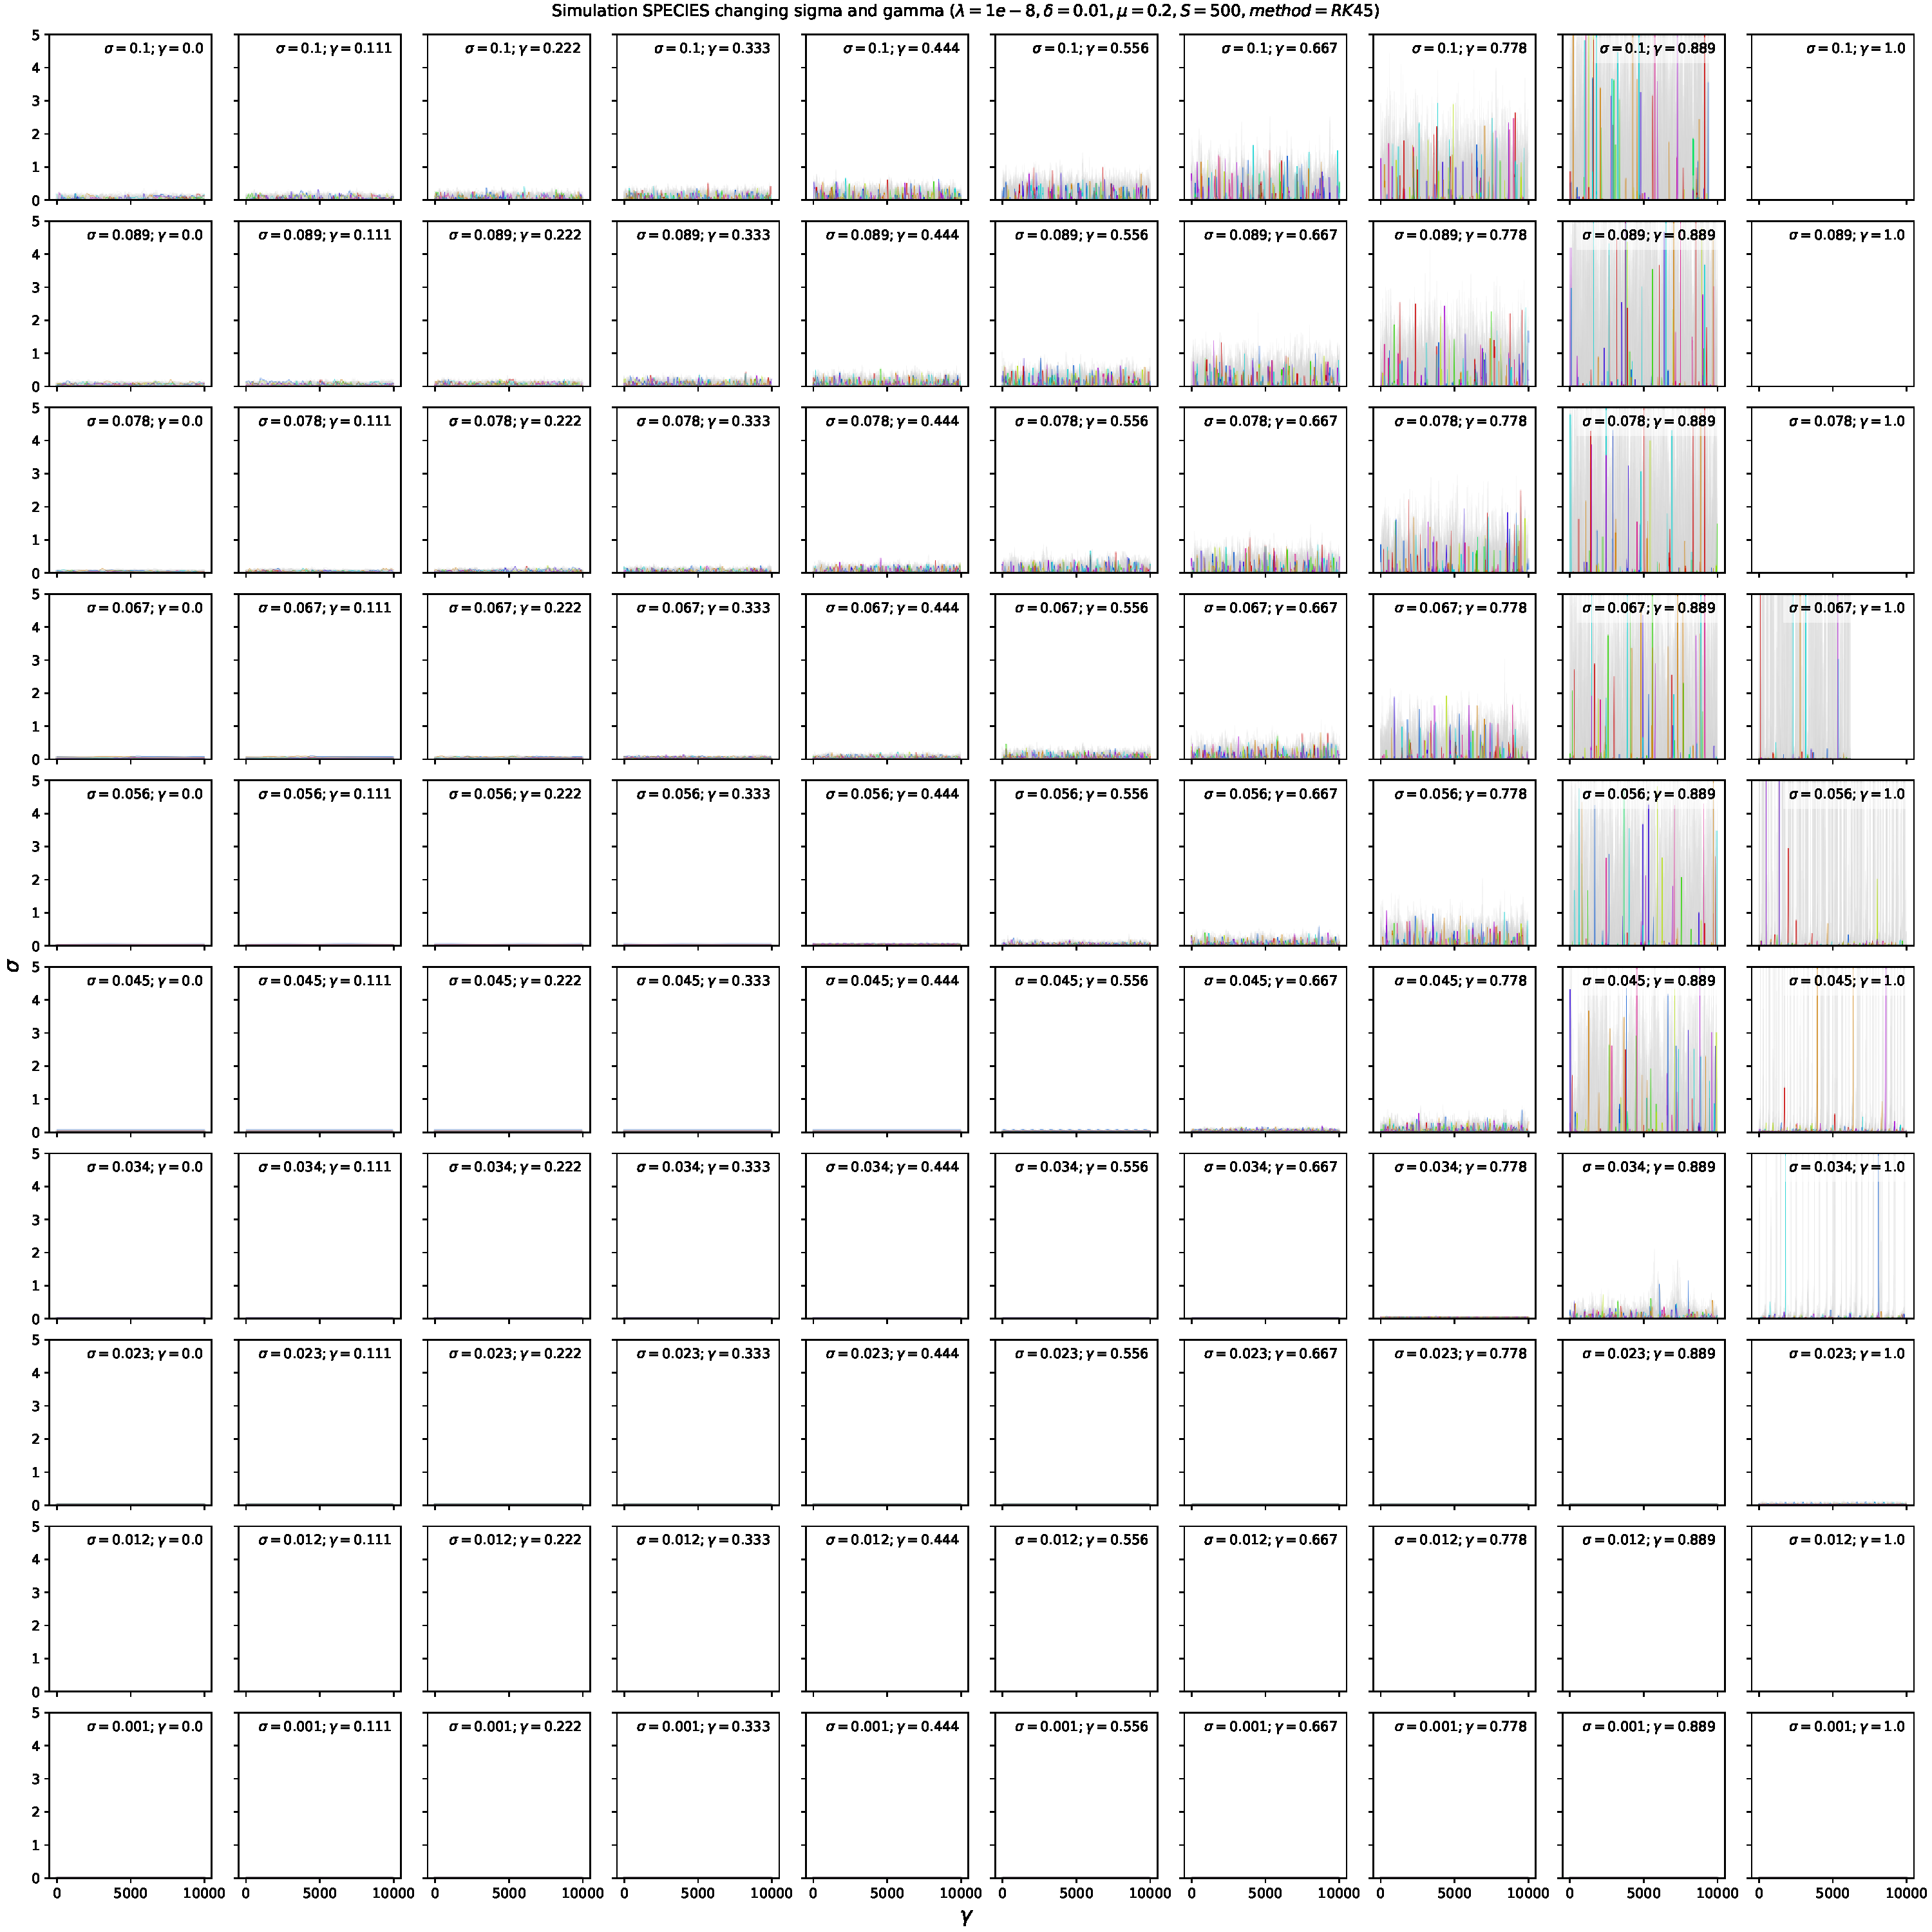
\includegraphics[width=\linewidth]{SigmaGamma/10SpeciesLinear.pdf}
    \caption{Species dynamics in linear scale $\sigma$ and $\gamma$.}
\end{figure}

\clearpage

\begin{figure}[H]
    \centering
    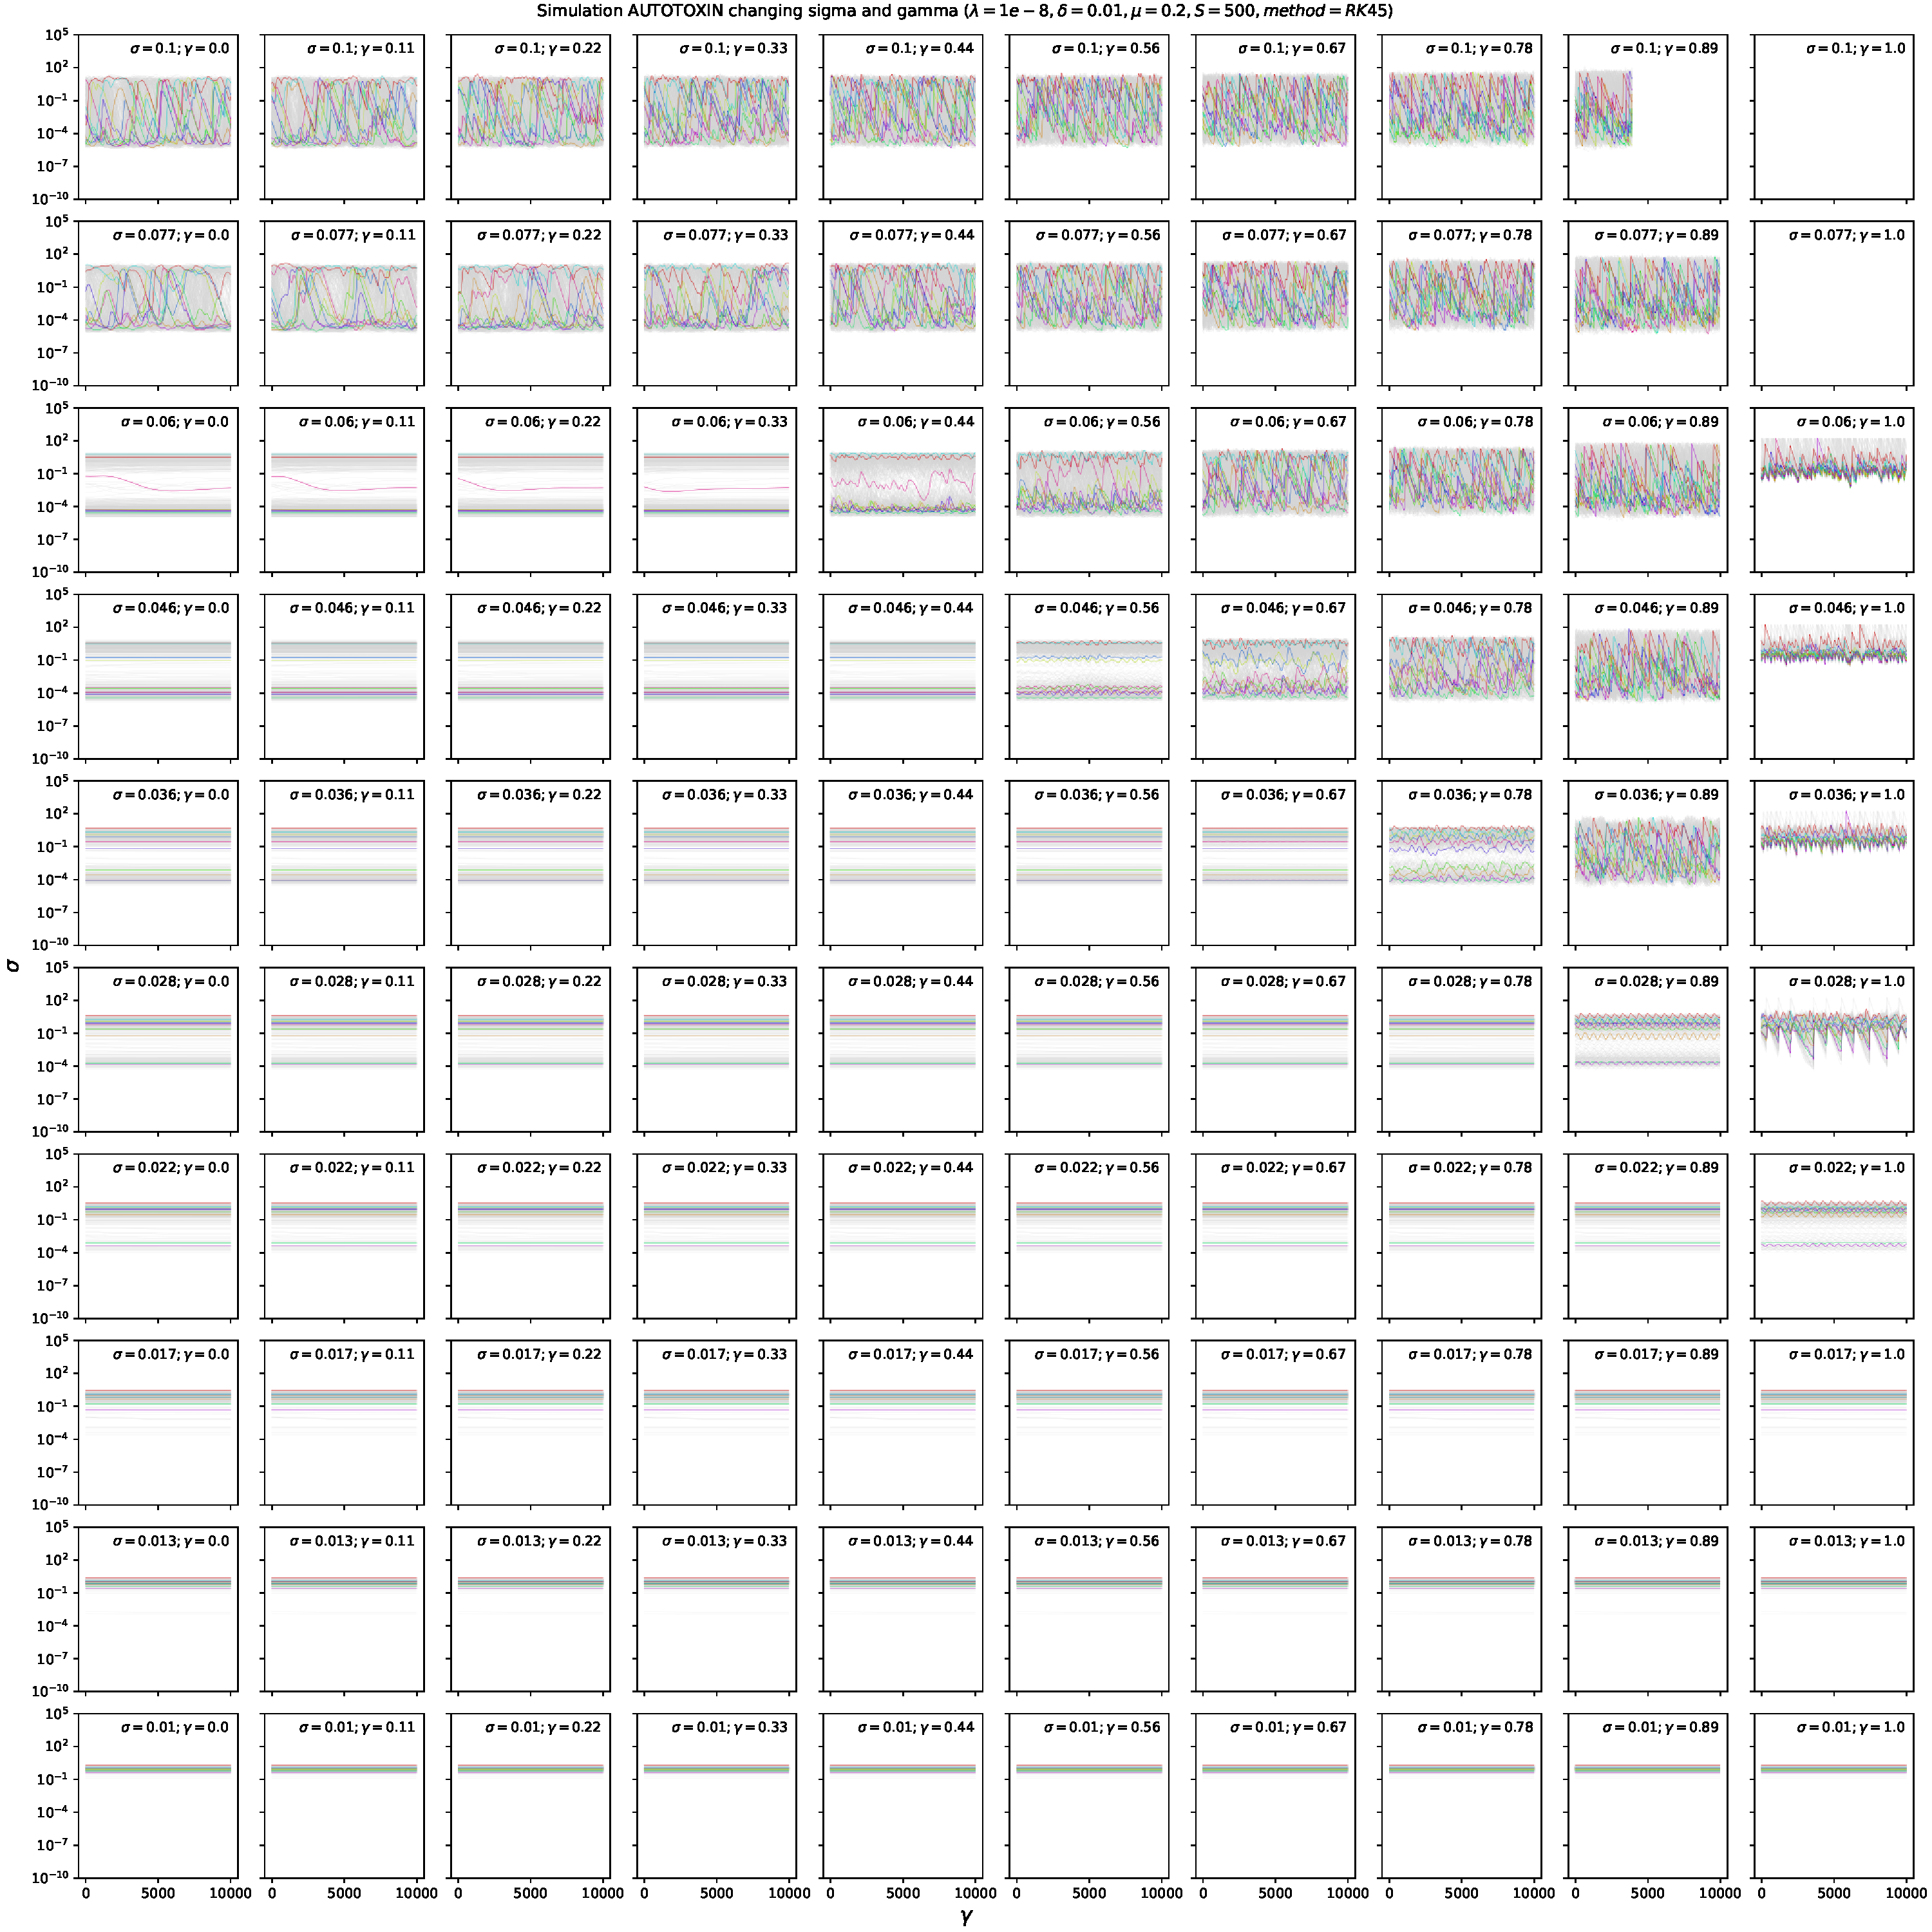
\includegraphics[width=\linewidth]{SigmaGamma/10Autotox.pdf}
    \caption{Autotoxin dynamics in logarithmic scale $\sigma$ and $\gamma$.}
\end{figure}

\clearpage

\begin{figure}[H]
    \centering
    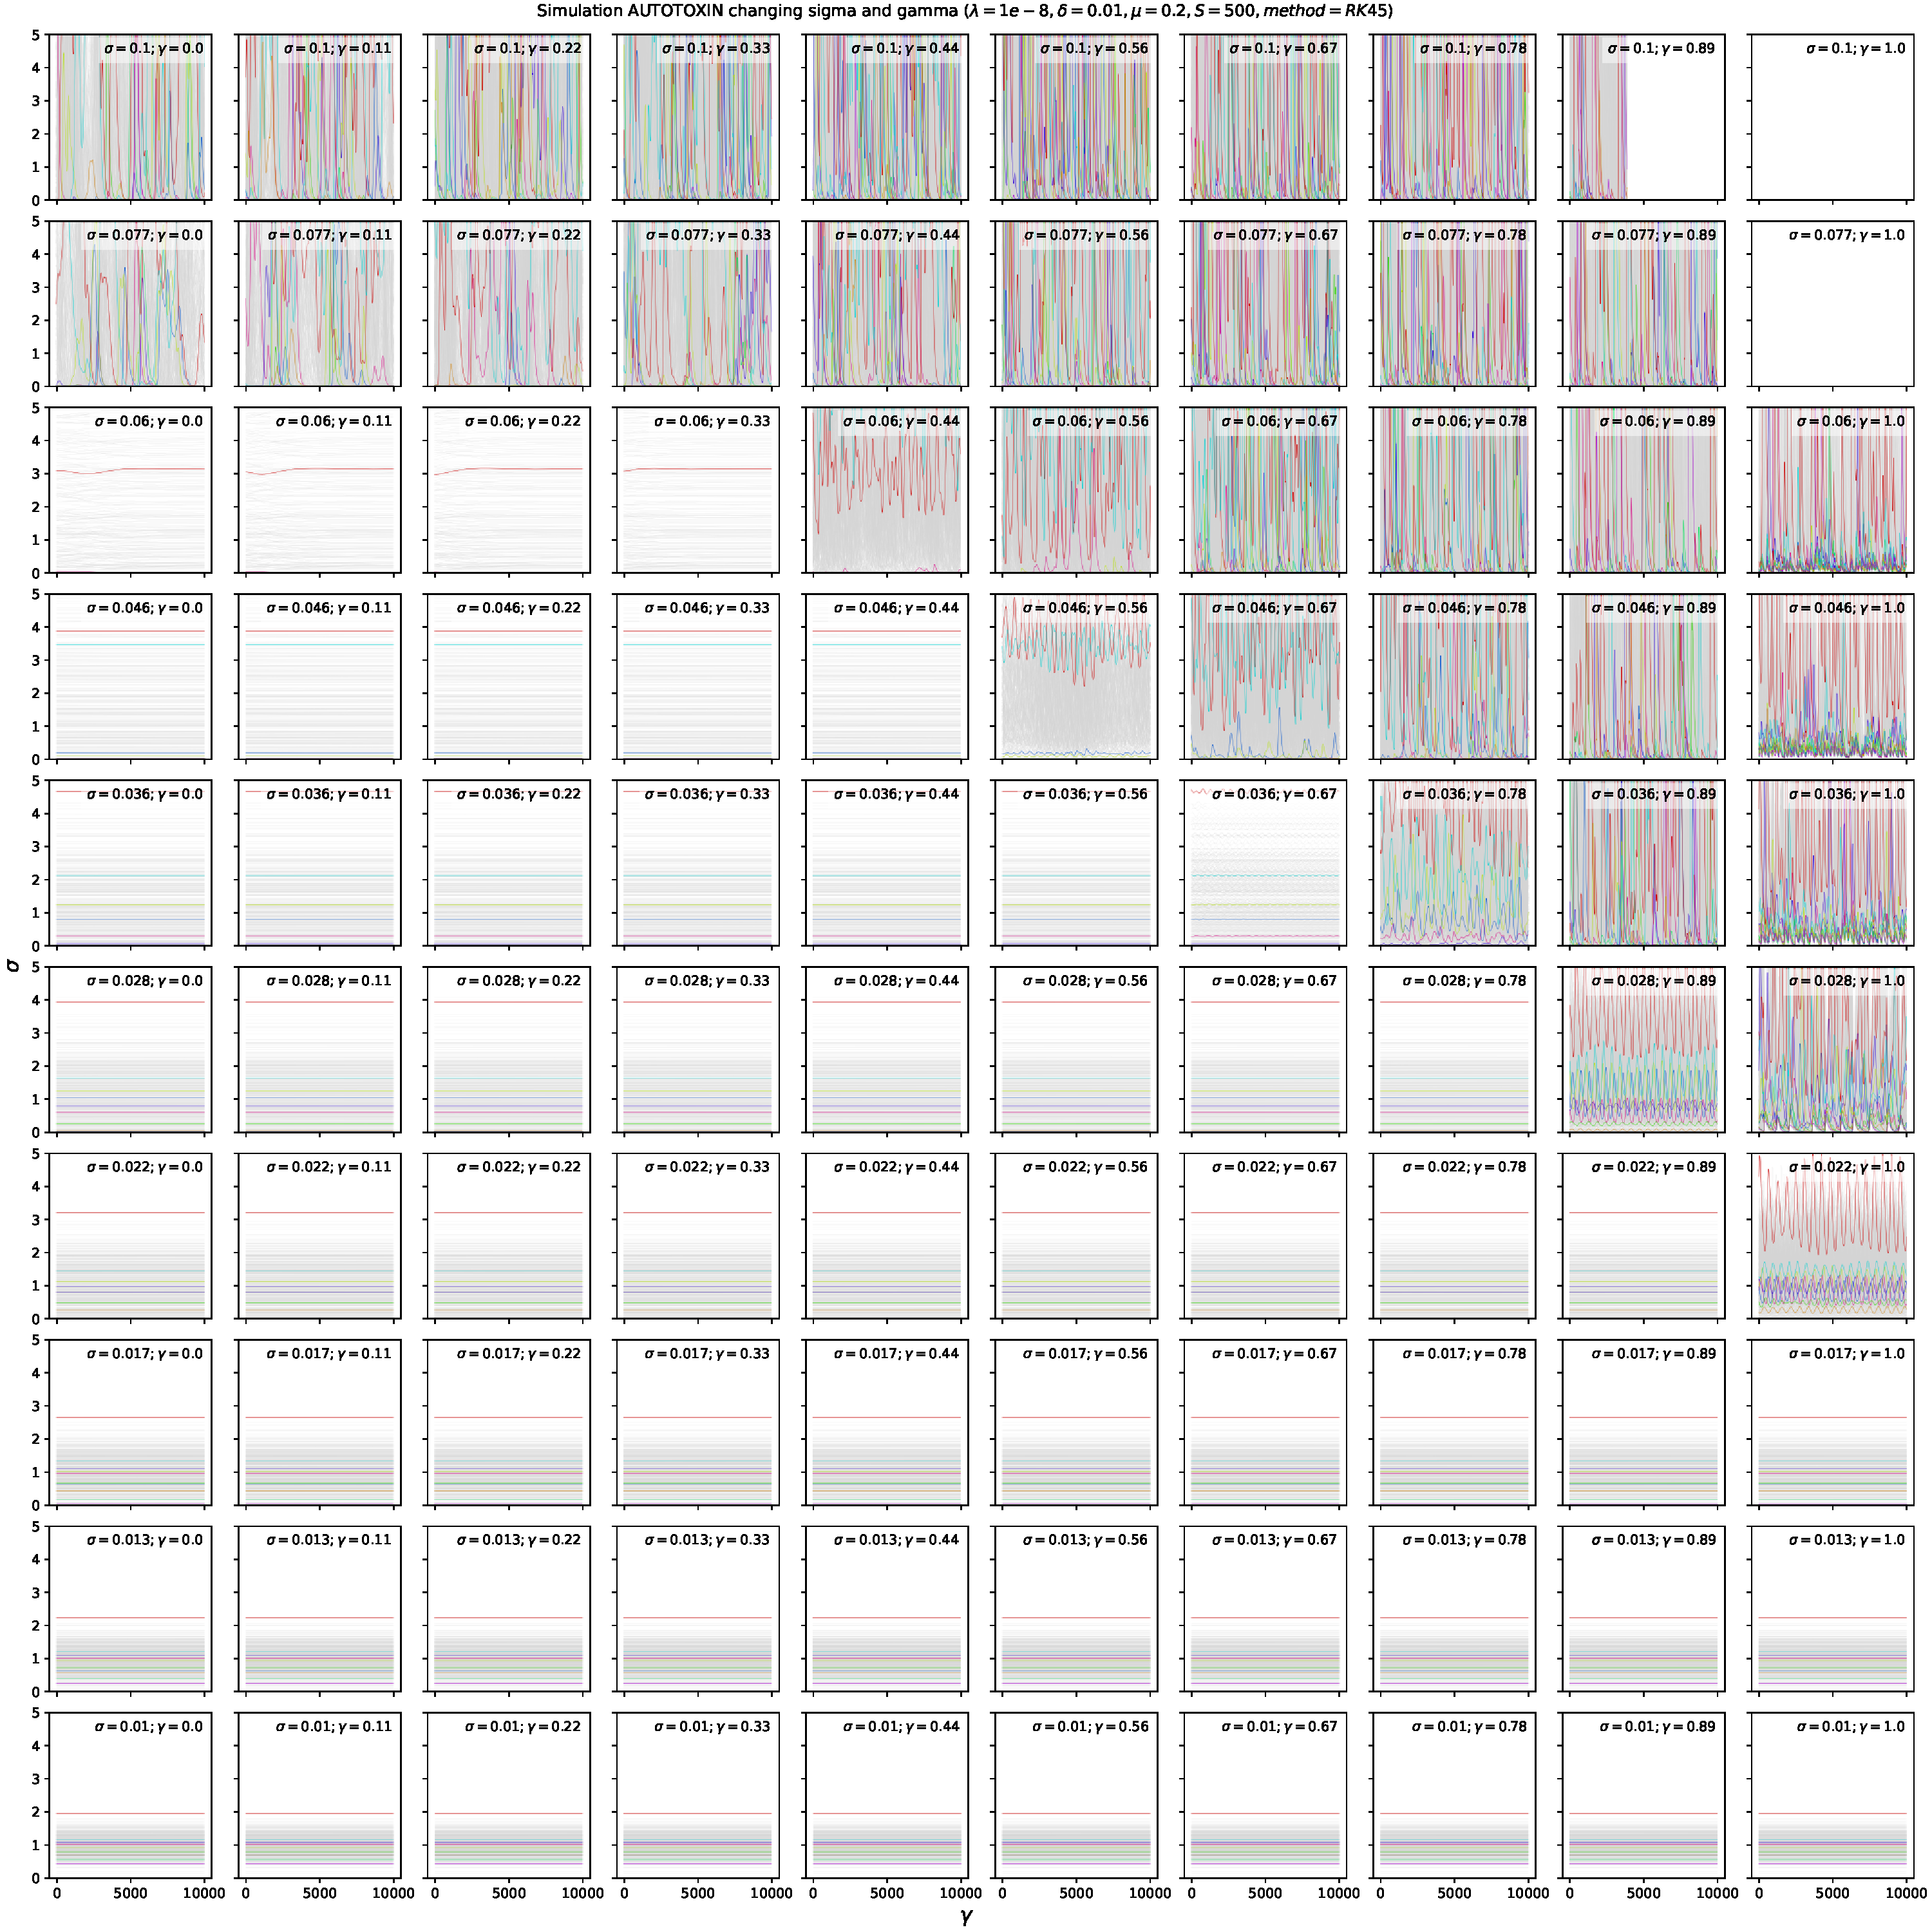
\includegraphics[width=\linewidth]{SigmaGamma/10AutotoxLinear.pdf}
    \caption{Autotoxin dynamics in linear scale $\sigma$ and $\gamma$.}
\end{figure}

\clearpage

The eigenvalues were evaluated at the last point of the simulation (e.g. after 10000 time steps) using the Jacobian calculated first in the log space and then in linear space
\begin{figure}[H]
    \centering
    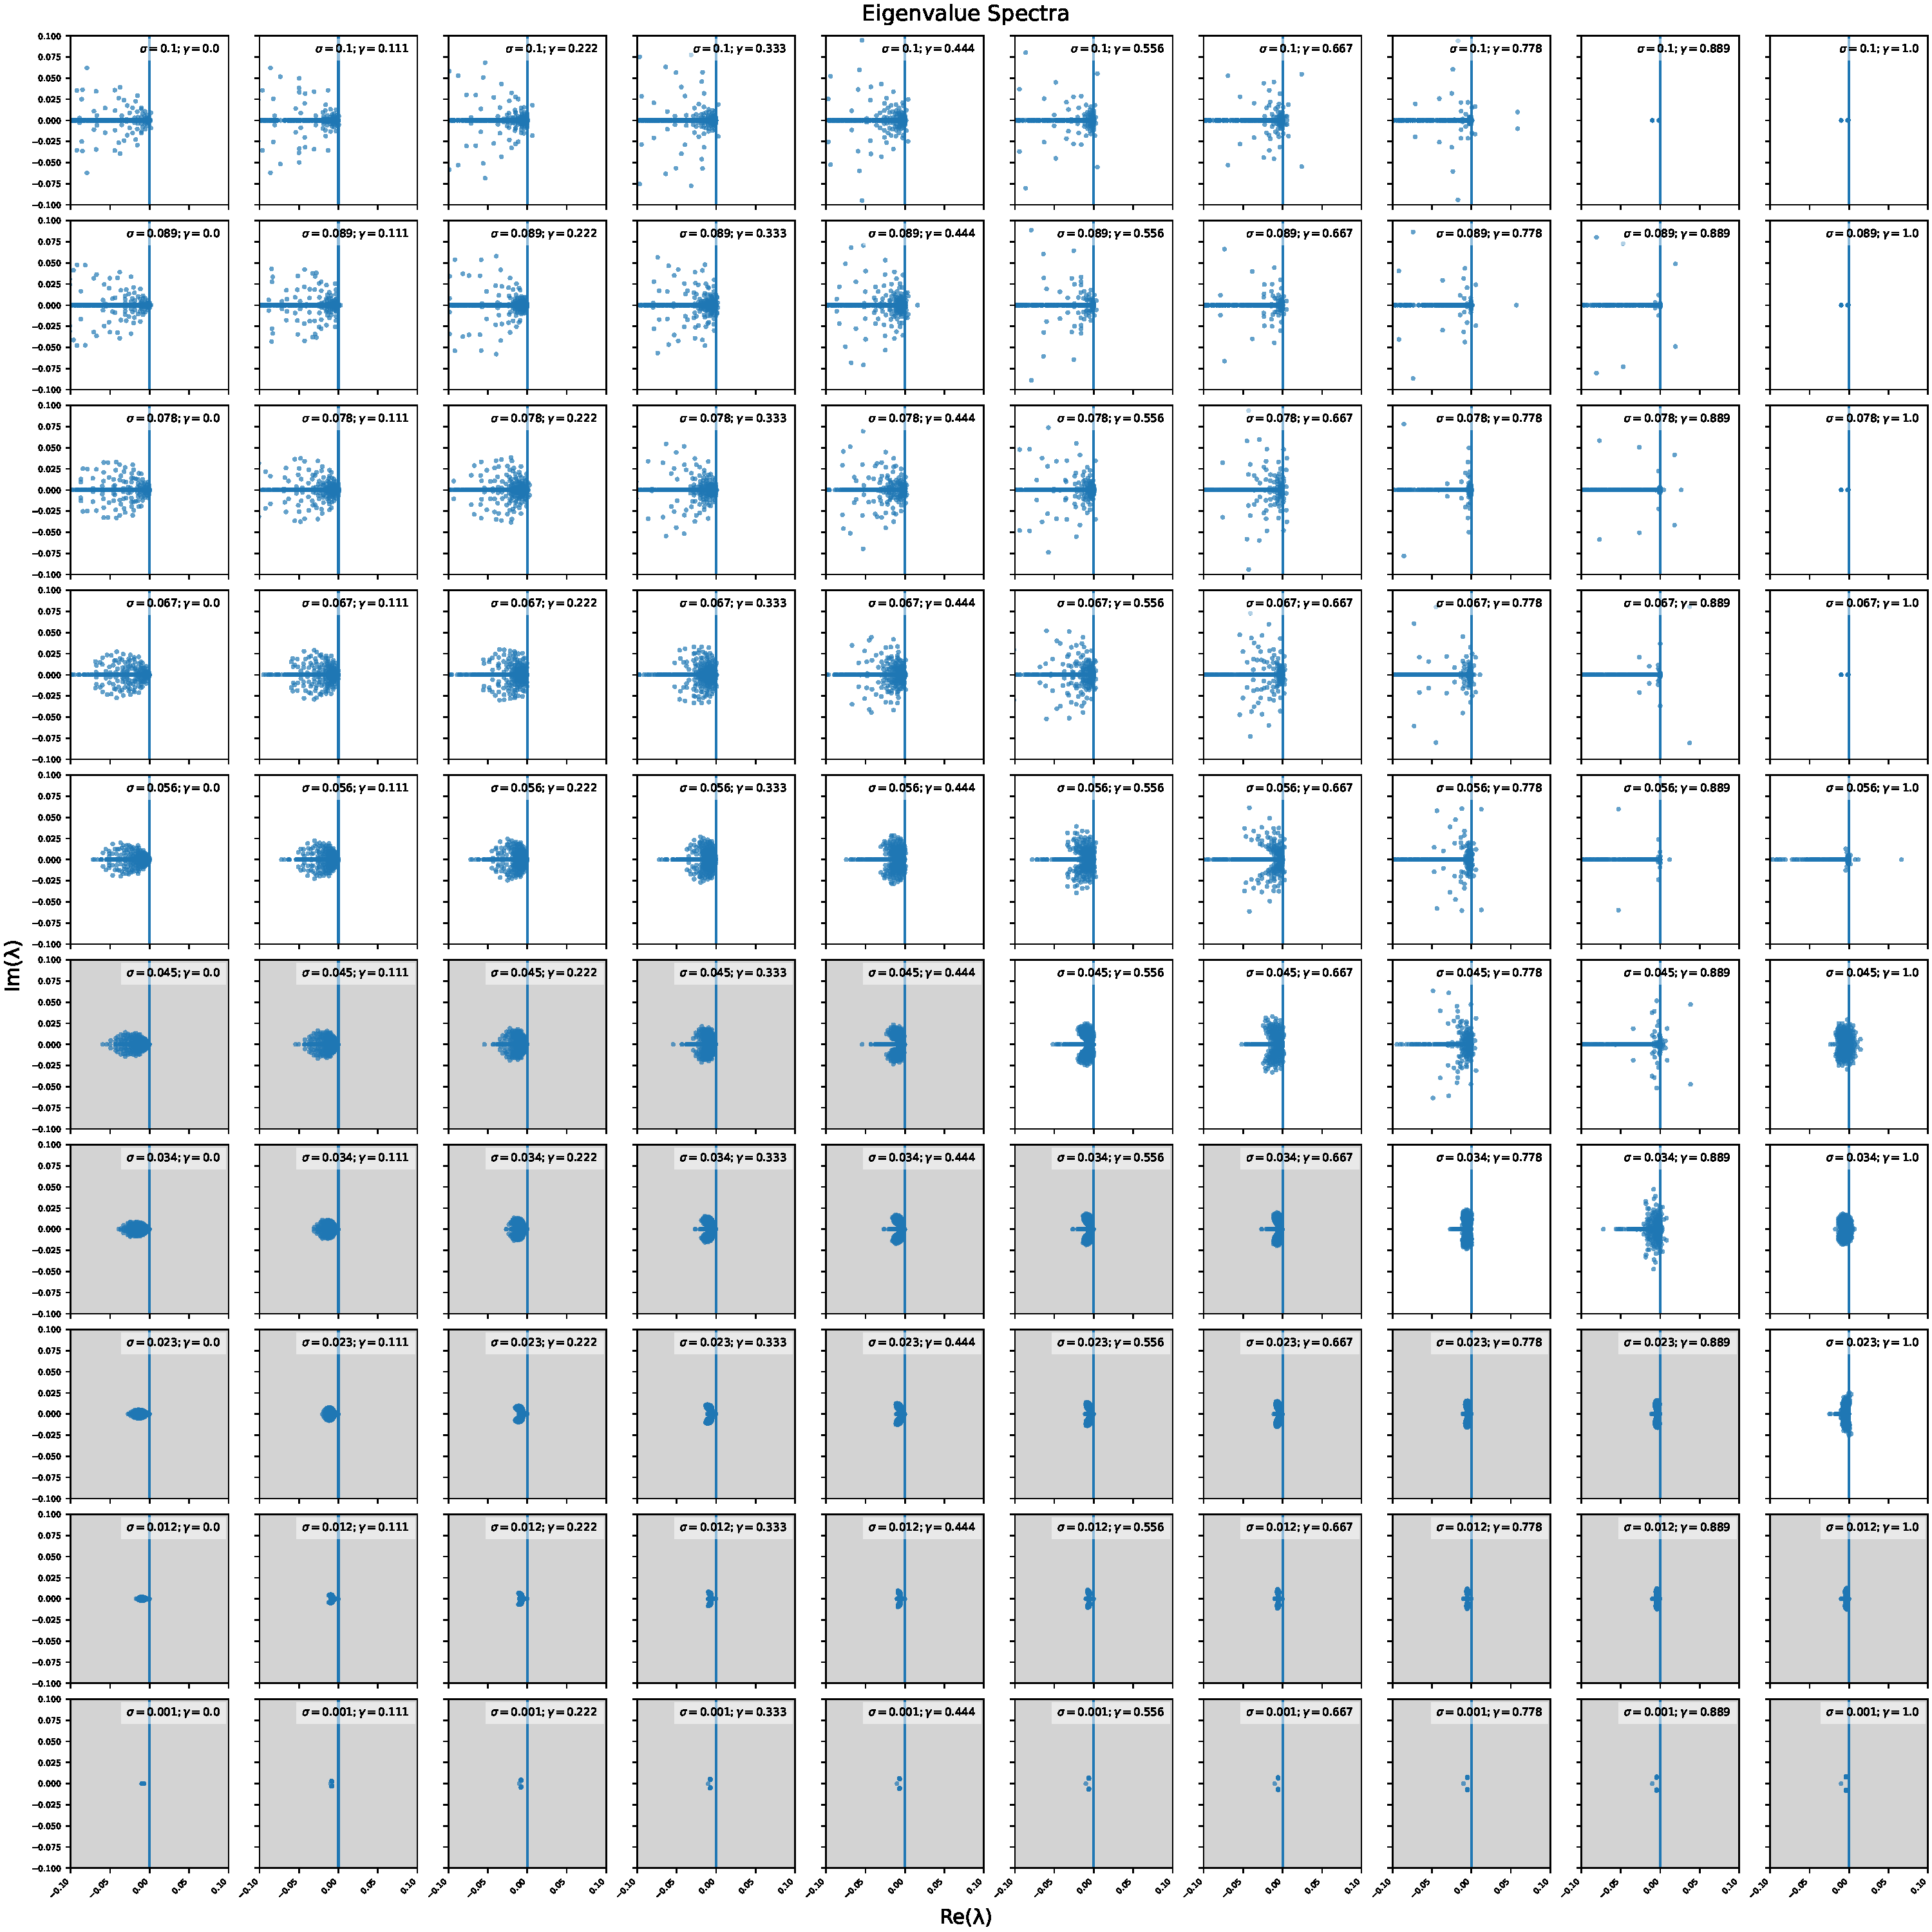
\includegraphics[width=\linewidth]{SigmaGamma/EigenValuesLogSigmaGamma.pdf}
    \caption{Eigenvalues by changing $\sigma$ and $\gamma$ using the jacobian evaluated for the state variables in the logarithmic space.}
\end{figure}

\begin{figure}[H]
    \centering
    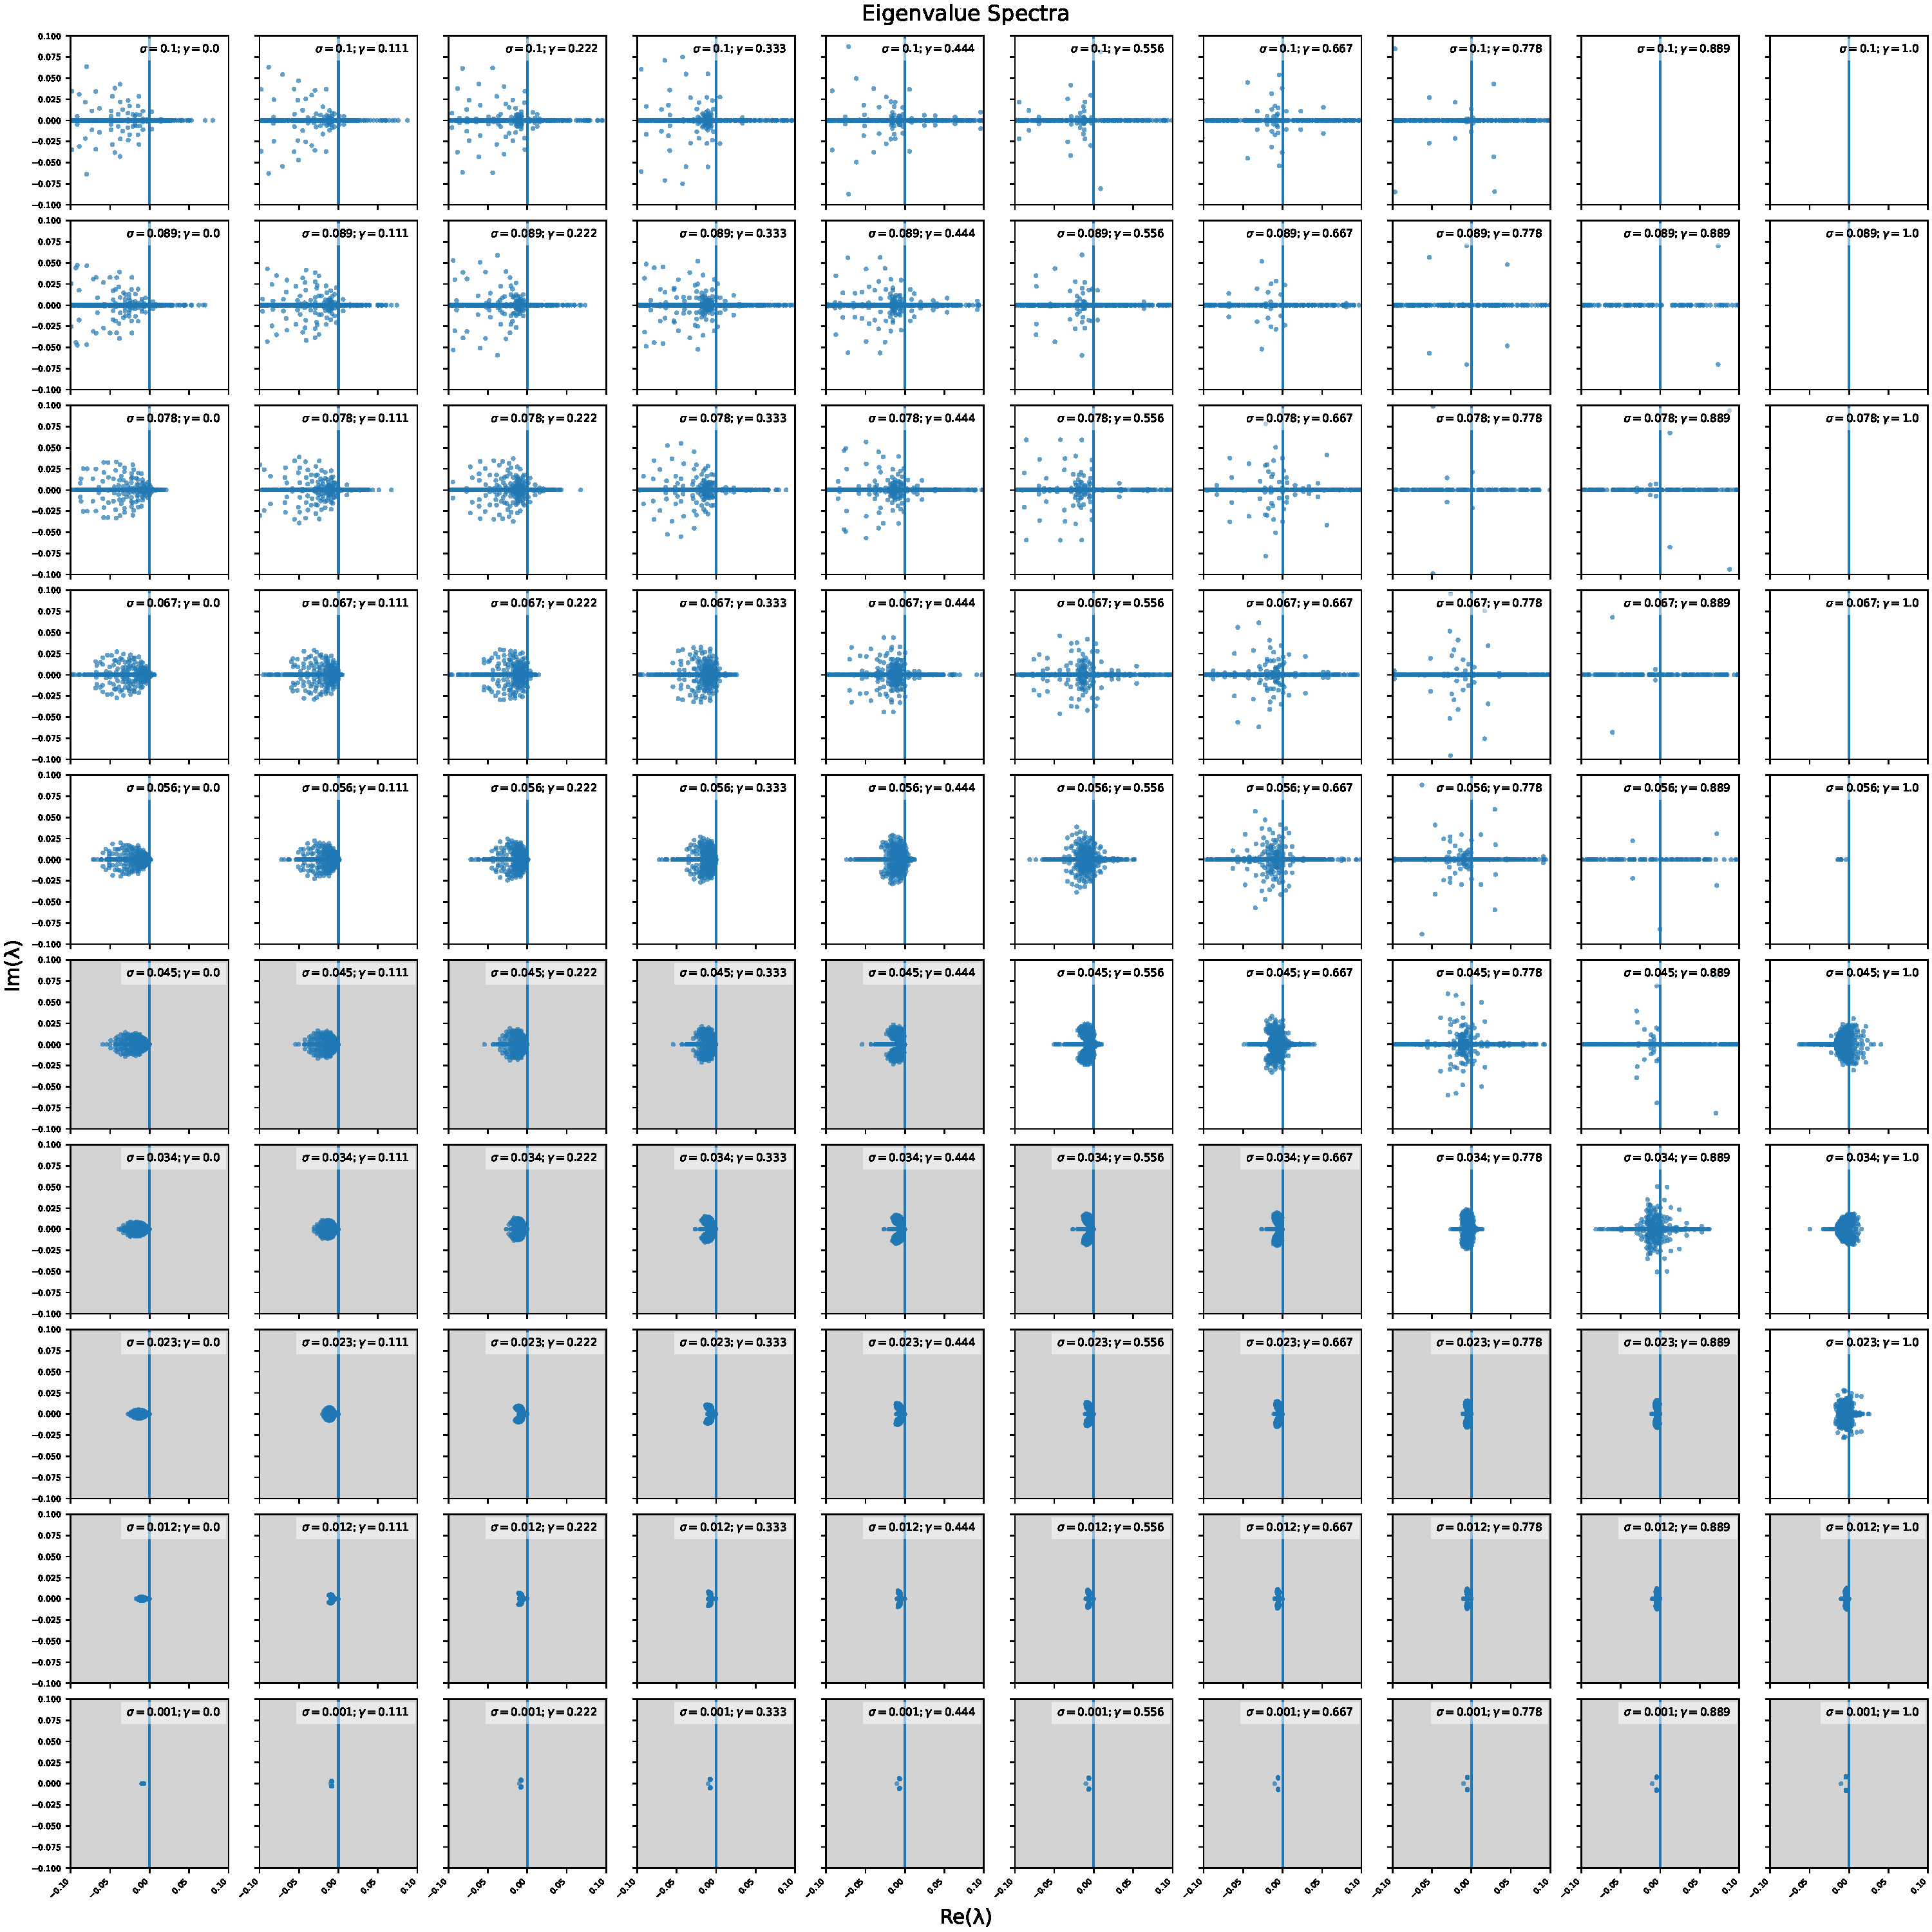
\includegraphics[width=\linewidth]{SigmaGamma/EigenValuesLinSigmaGamma.pdf}
    \caption{Eigenvalues by changing $\sigma$ and $\gamma$ using the jacobian evaluated for the state variables in the linear space.}
\end{figure}
\clearpage

\paragraph{Simulations $\delta$ $\gamma$}

\[
C_{ij} \sim \mathcal{N}(0.23, 0.05), \quad 
\delta \in [0.001, 1], \quad 
\gamma \in [0, 1], \quad \lambda = 10^{-8}
\]

\begin{figure}[H]
    \centering
    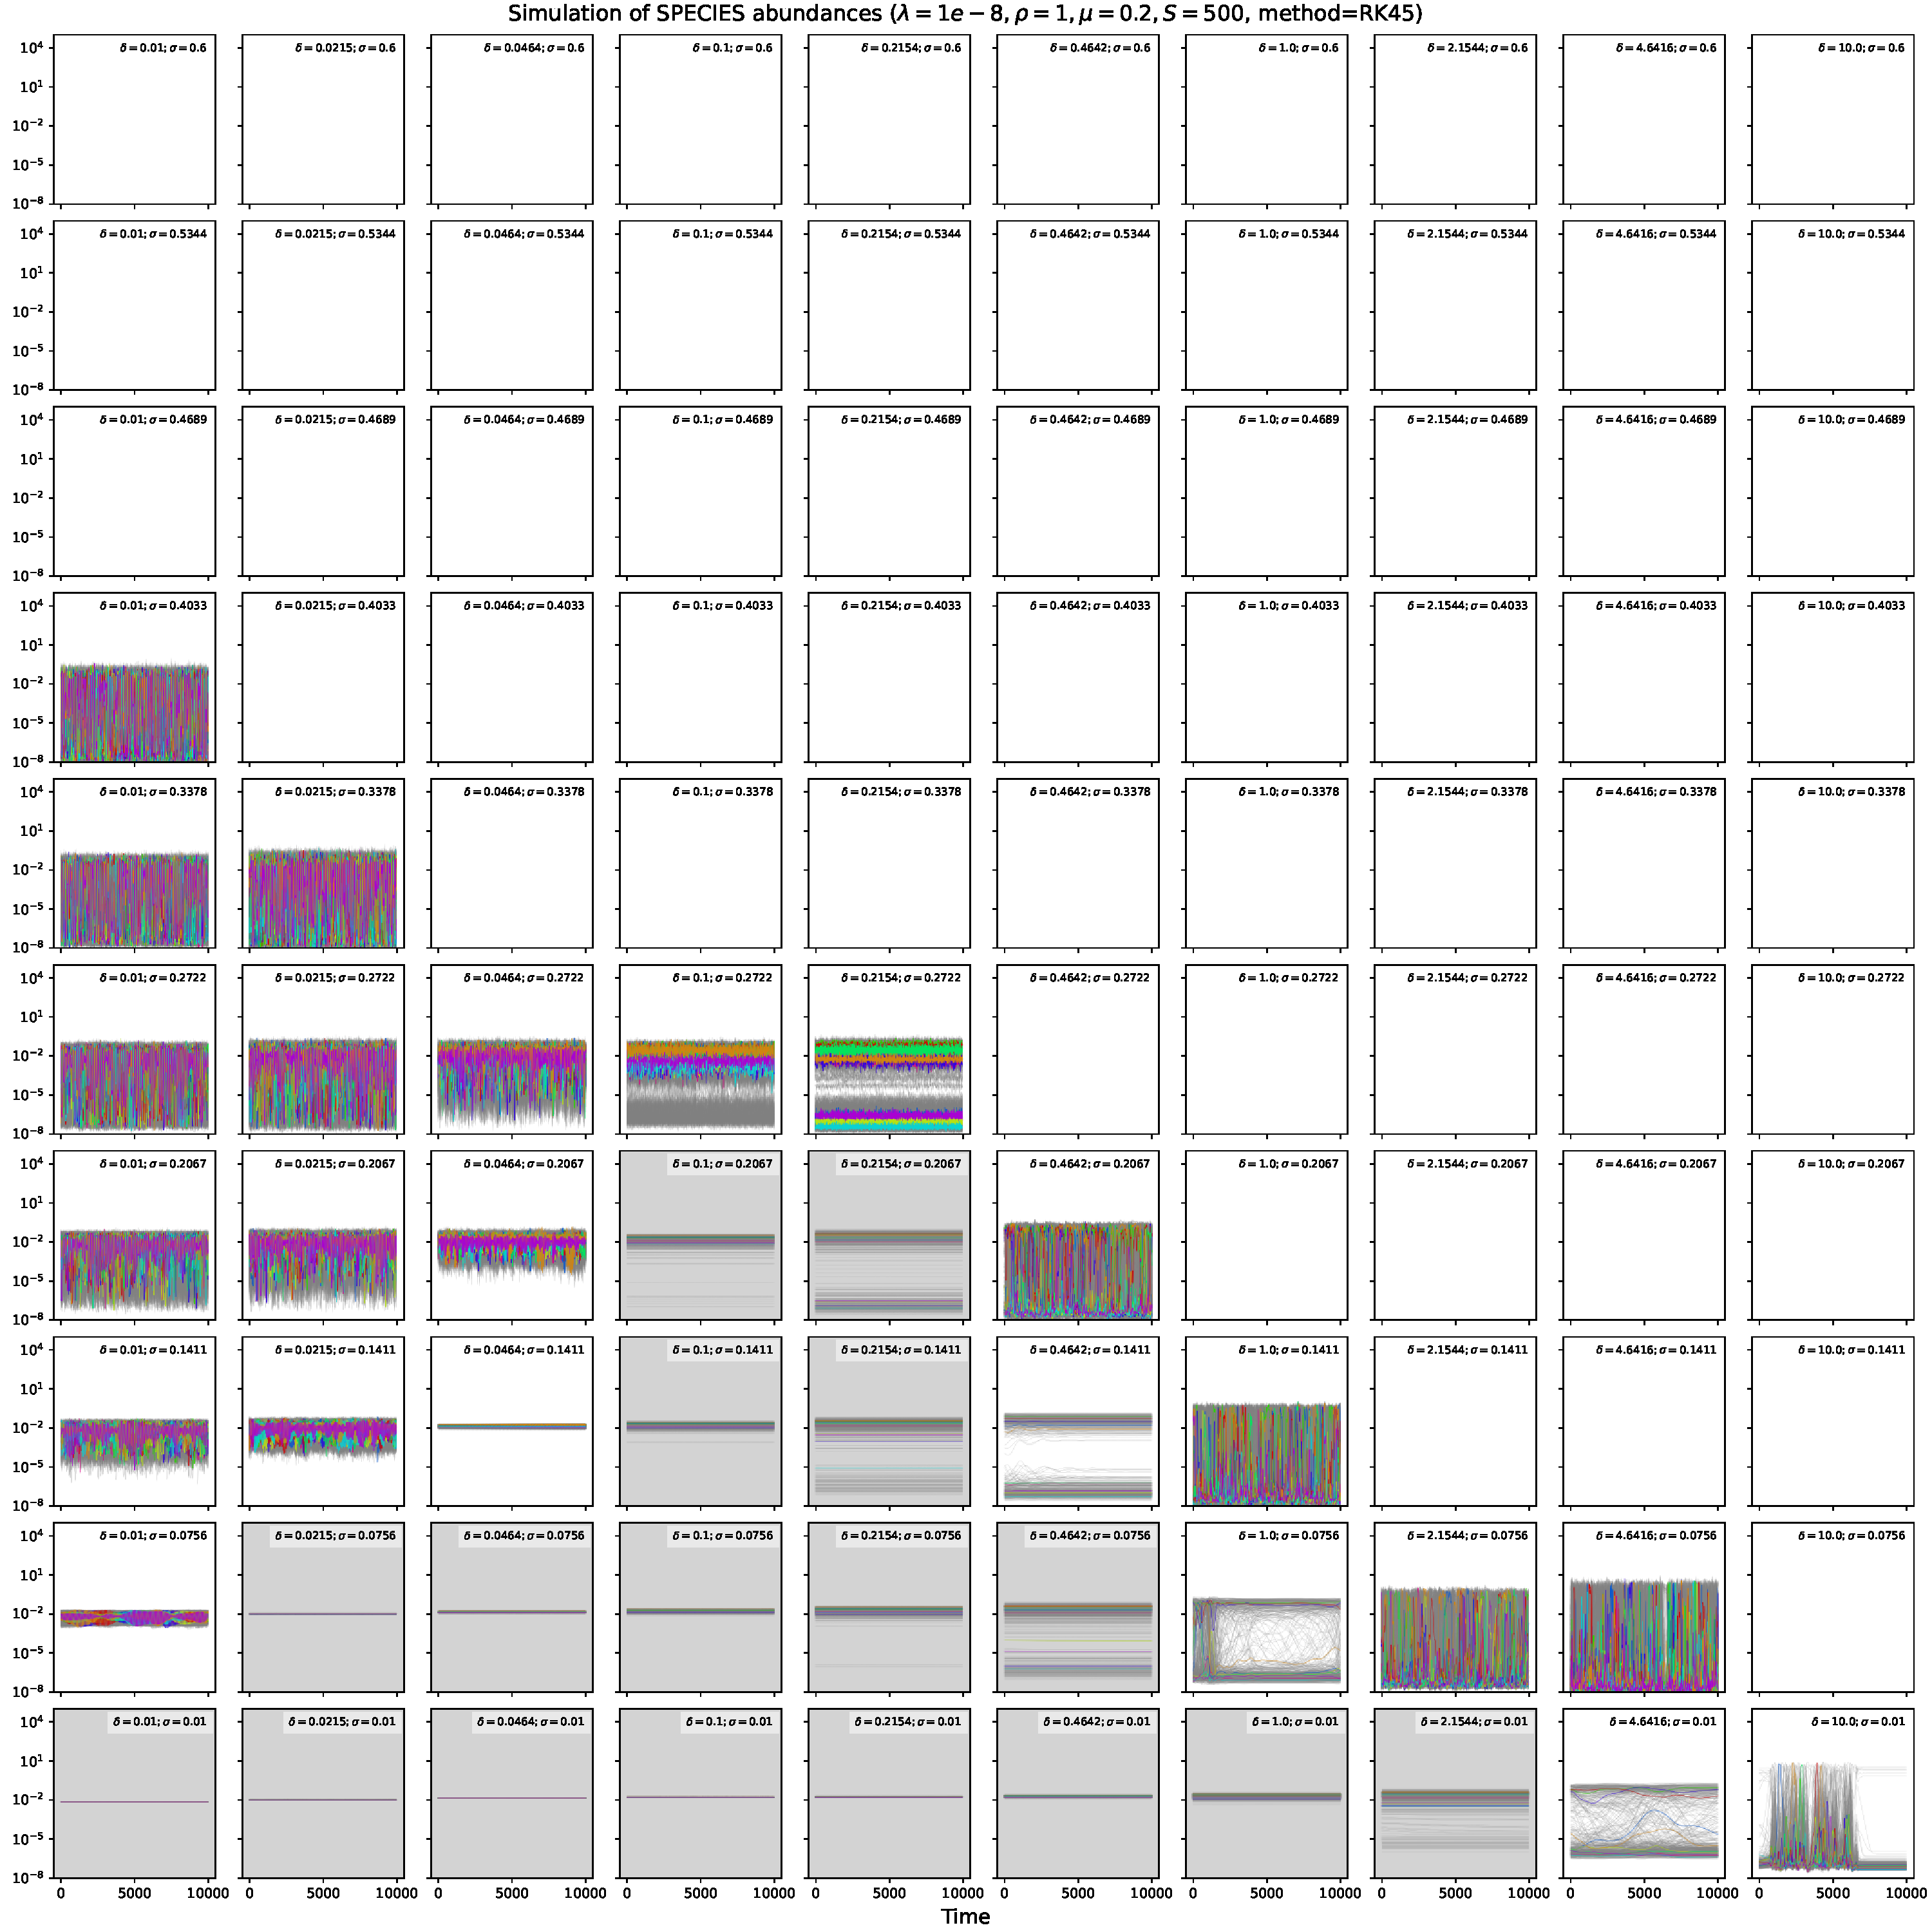
\includegraphics[width=\linewidth]{DeltaGamma/10SpeciesFP.pdf}
    \caption{Species dynamics in logarithmic scale changing $\delta$ and $\gamma$.}
\end{figure}

\clearpage

\begin{figure}[H]
    \centering
    \includegraphics[width=\linewidth]{DeltaGamma/10SpeciesFPLinear.pdf}
    \caption{Species dynamics in linear scale changing $\delta$ and $\gamma$.}
\end{figure}

\clearpage

\begin{figure}[H]
    \centering
    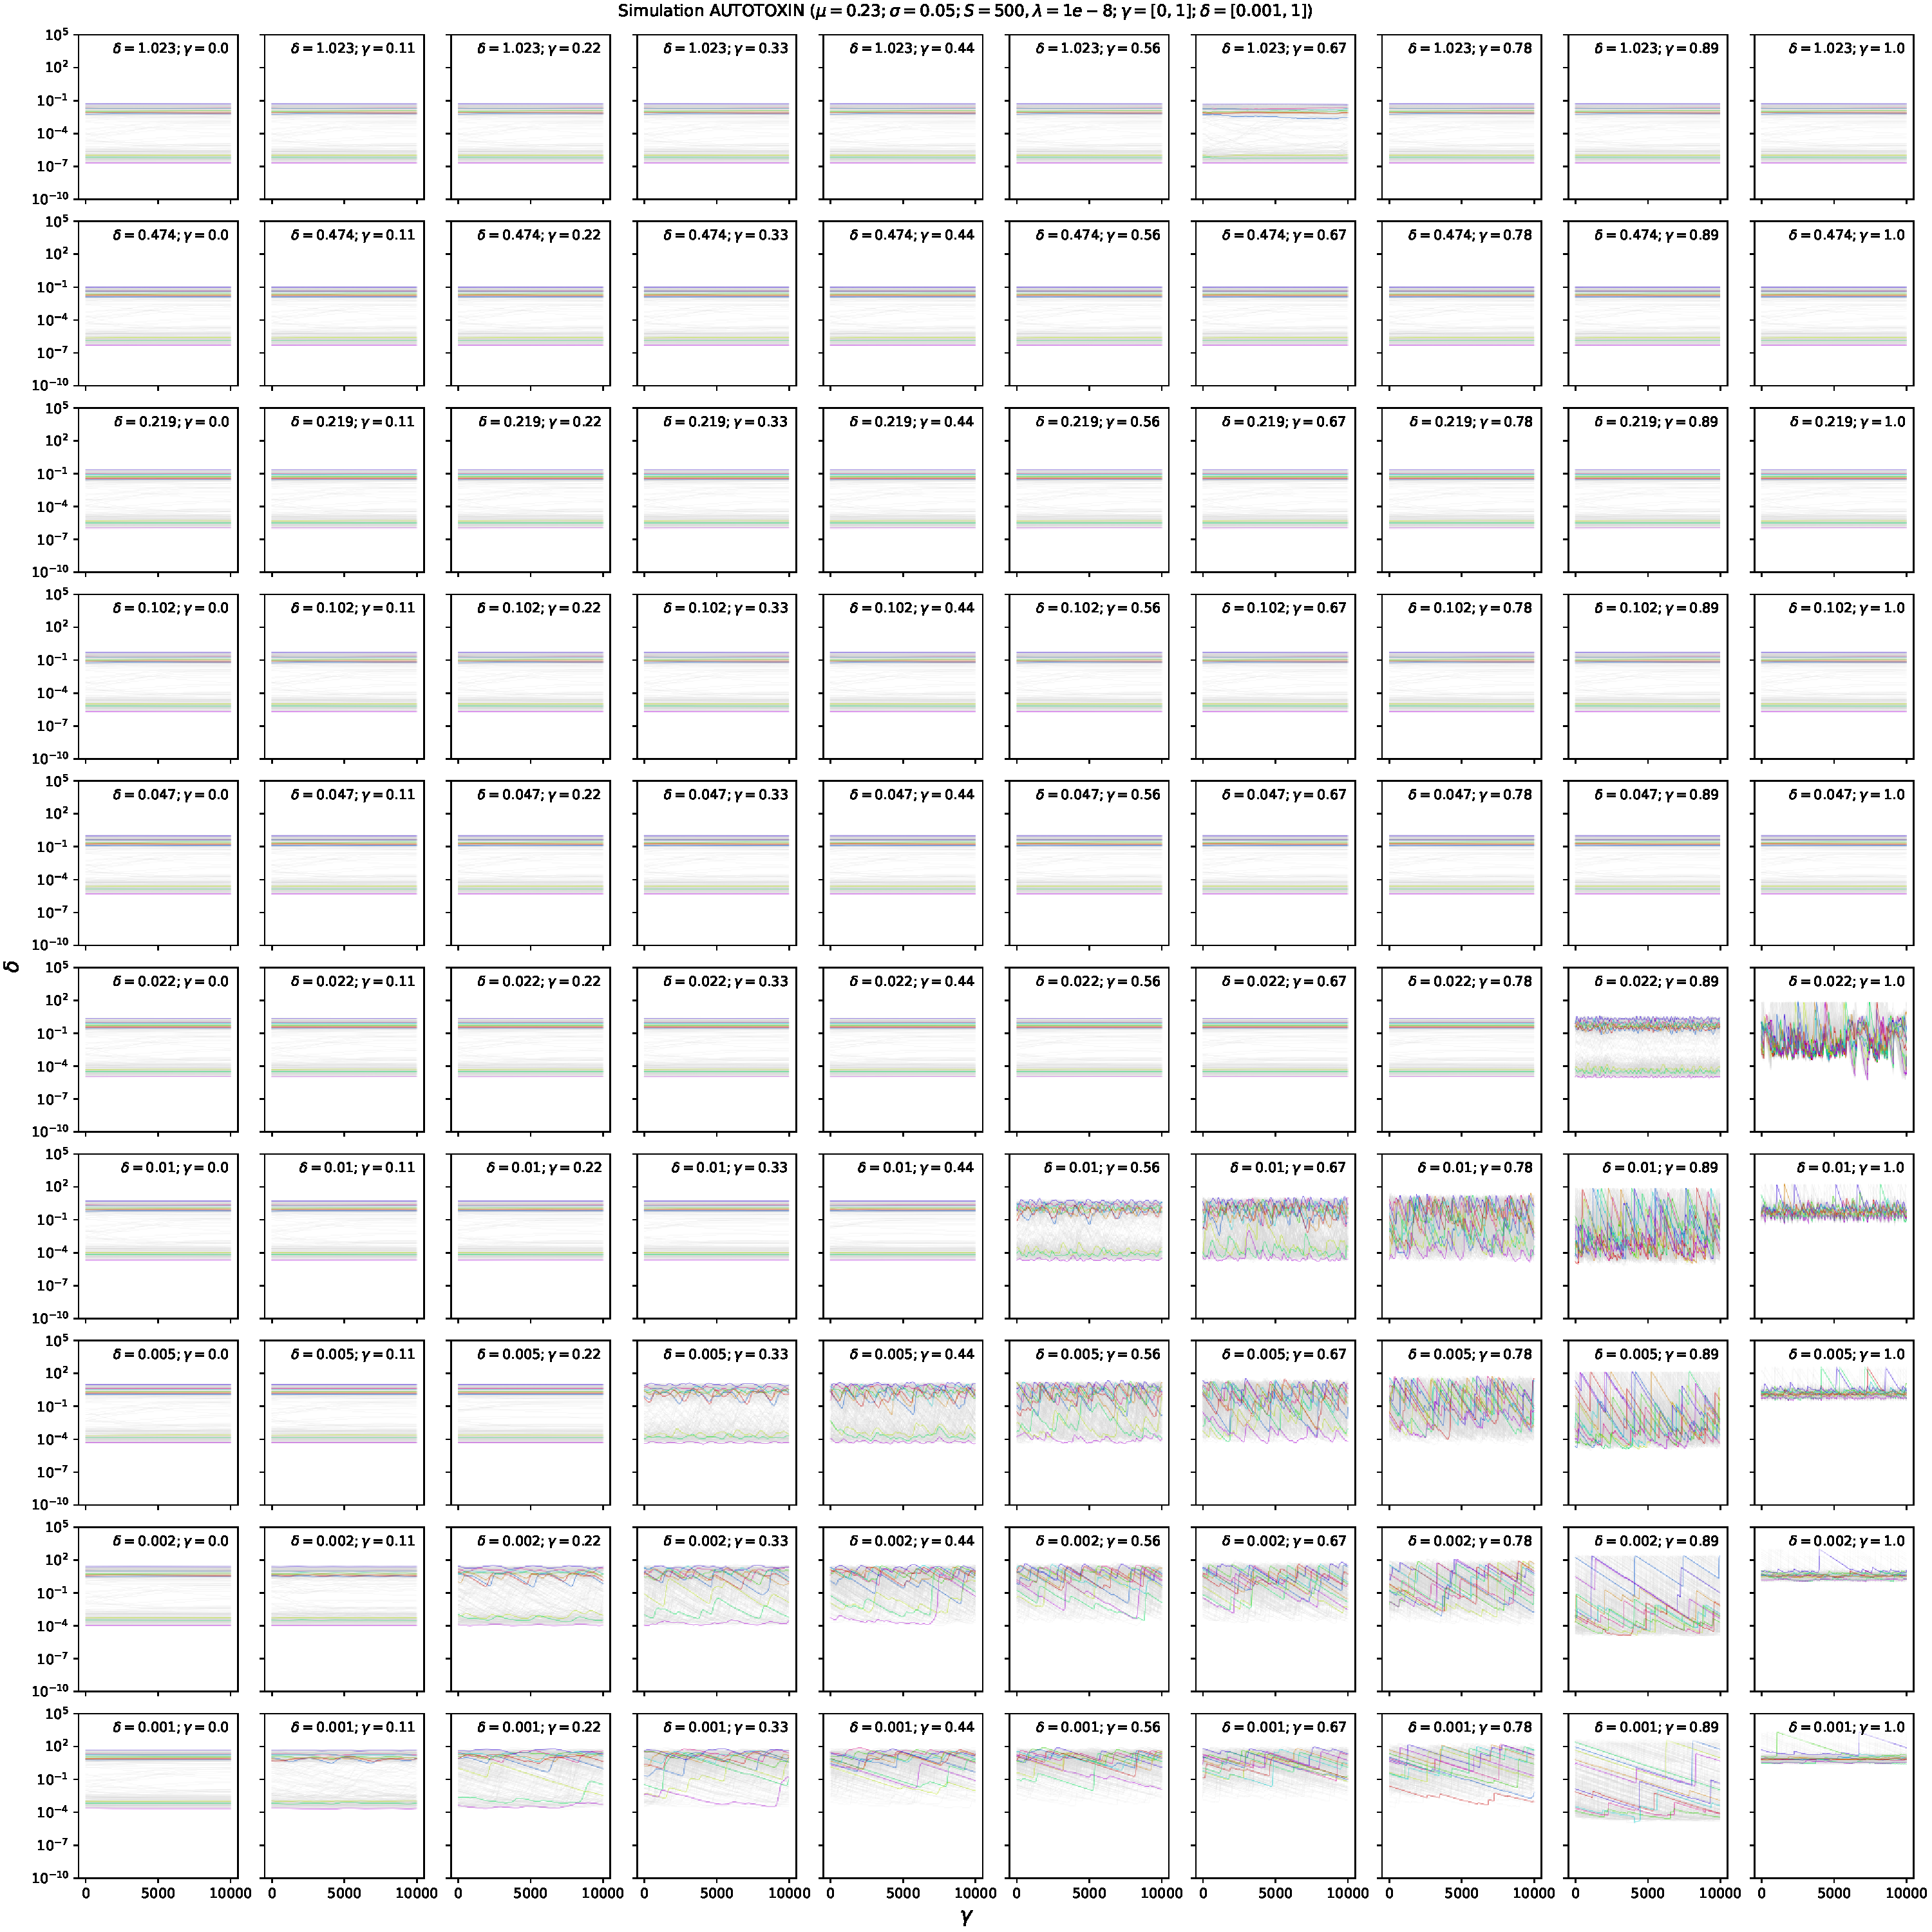
\includegraphics[width=\linewidth]{DeltaGamma/10autotoxFP.pdf}
    \caption{Autotoxin dynamics in logarithmic scale changing $\delta$ and $\gamma$.}
\end{figure}

\clearpage

\begin{figure}[H]
    \centering
    \includegraphics[width=\linewidth]{DeltaGamma/10AutotoxFPLinear.pdf}
    \caption{Autotoxin dynamics in linear scale changing $\delta$ and $\gamma$.}
\end{figure}

\clearpage
\subparagraph{Eigen Values $\delta$ $\gamma$}

Again, the eigenvalues were evaluated at the last point of the simulation (e.g. after 10000 time steps) using the Jacobian calculated first in the log space and then in linear space

\begin{figure}[H]
    \centering
    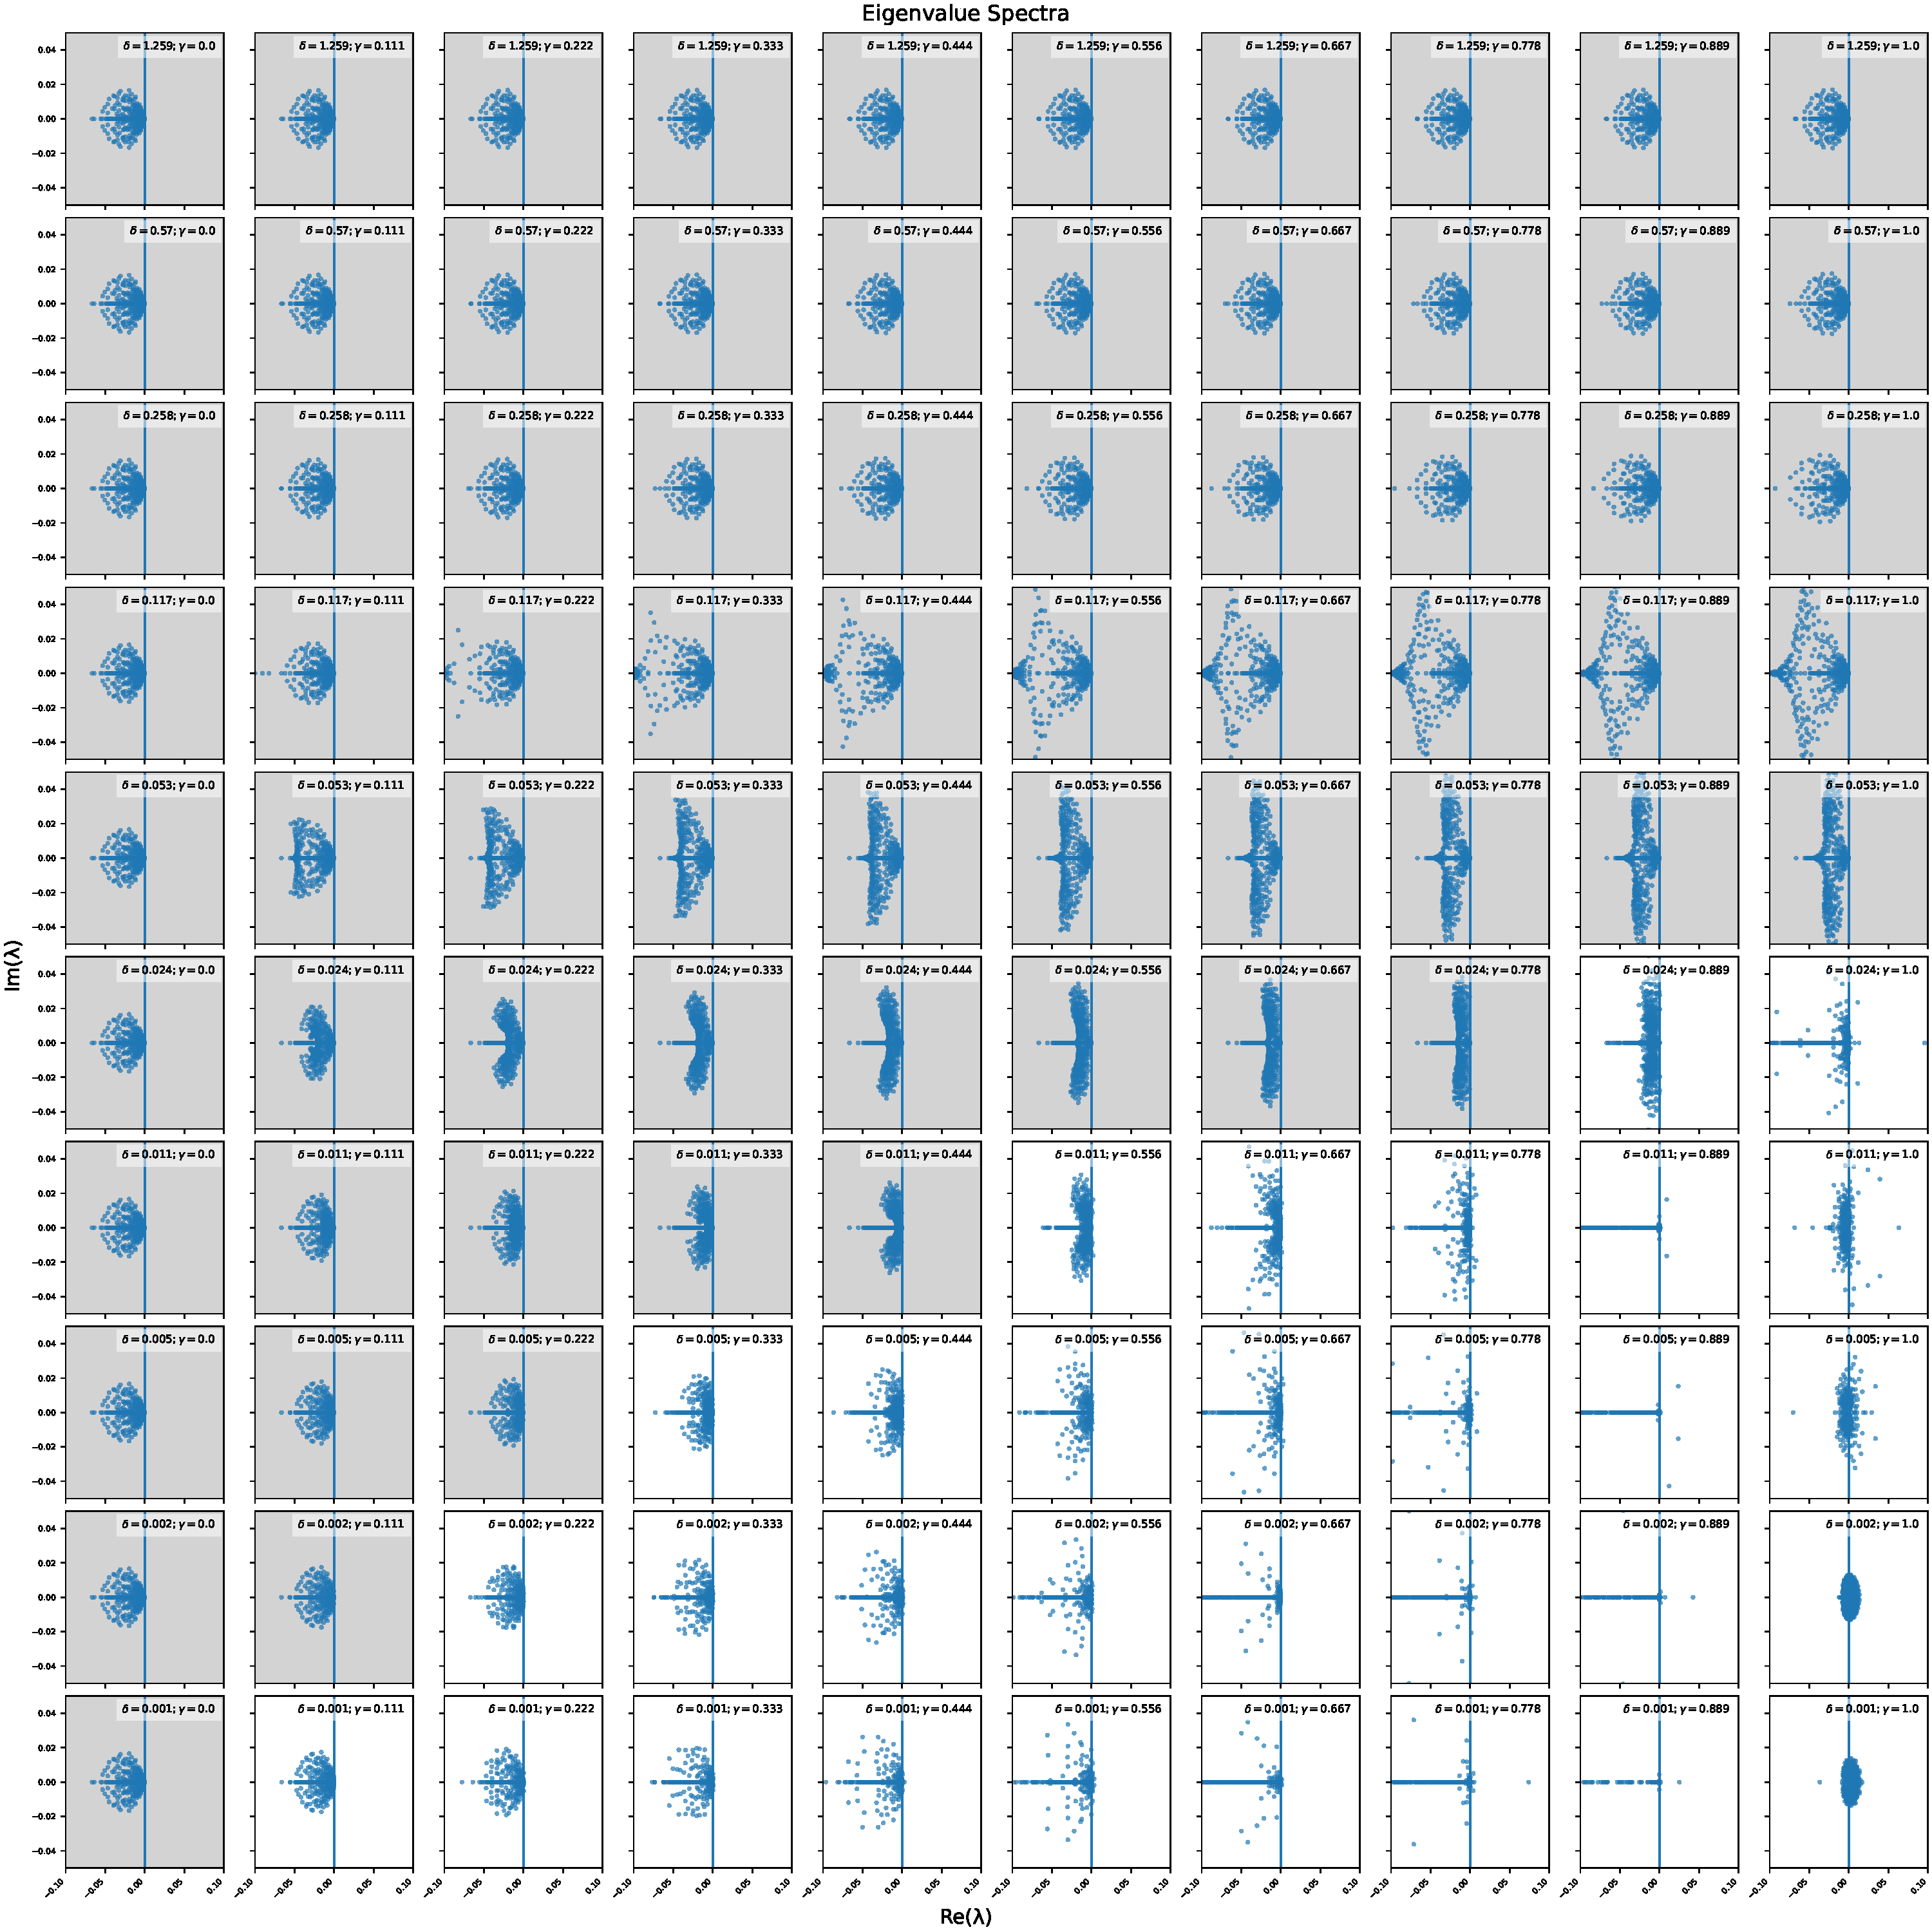
\includegraphics[width=\linewidth]{DeltaGamma/EigenValuesDeltaGammaLog.pdf}
    \caption{Eigenvalues by changing $\delta$ and $\gamma$.}
\end{figure}


\begin{figure}[H]
    \centering
    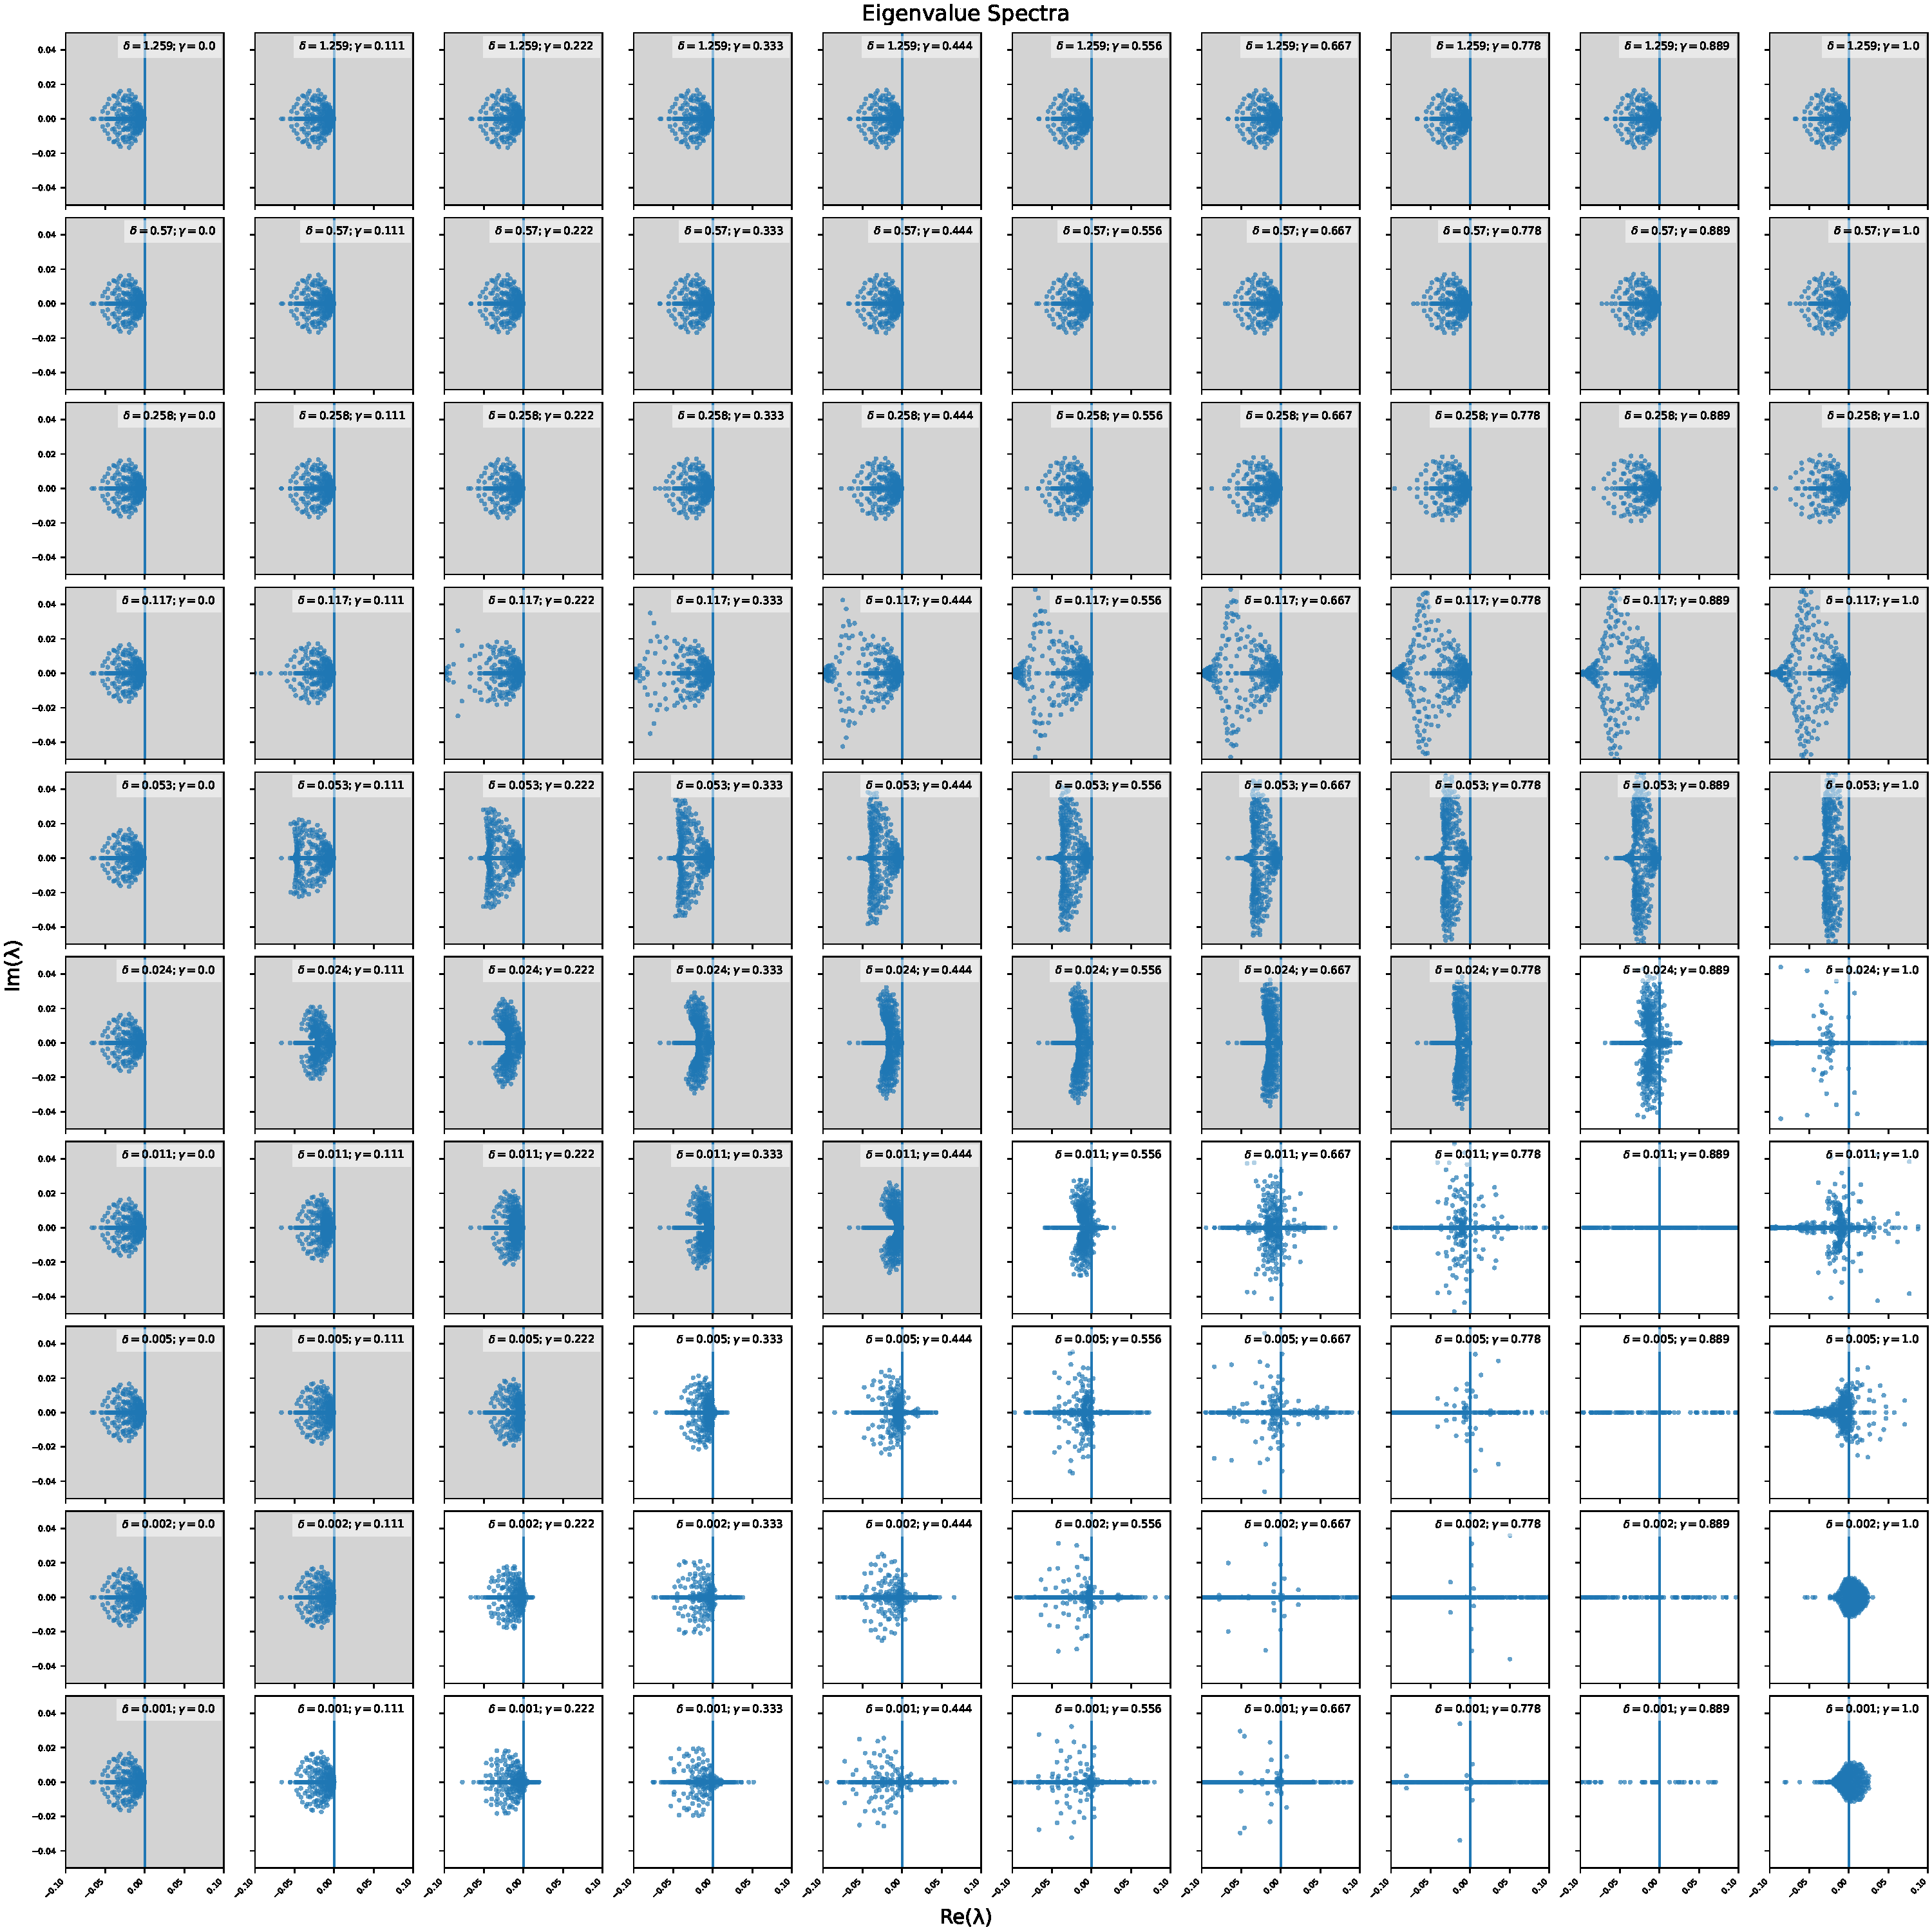
\includegraphics[width=\linewidth]{DeltaGamma/EigenValuesDeltaGammaLin.pdf}
    \caption{Eigenvalues by changing $\delta$ and $\gamma$.}
\end{figure}

\clearpage


\paragraph{Bifurcation Analysis}

\begin{figure}[H]
    \centering
    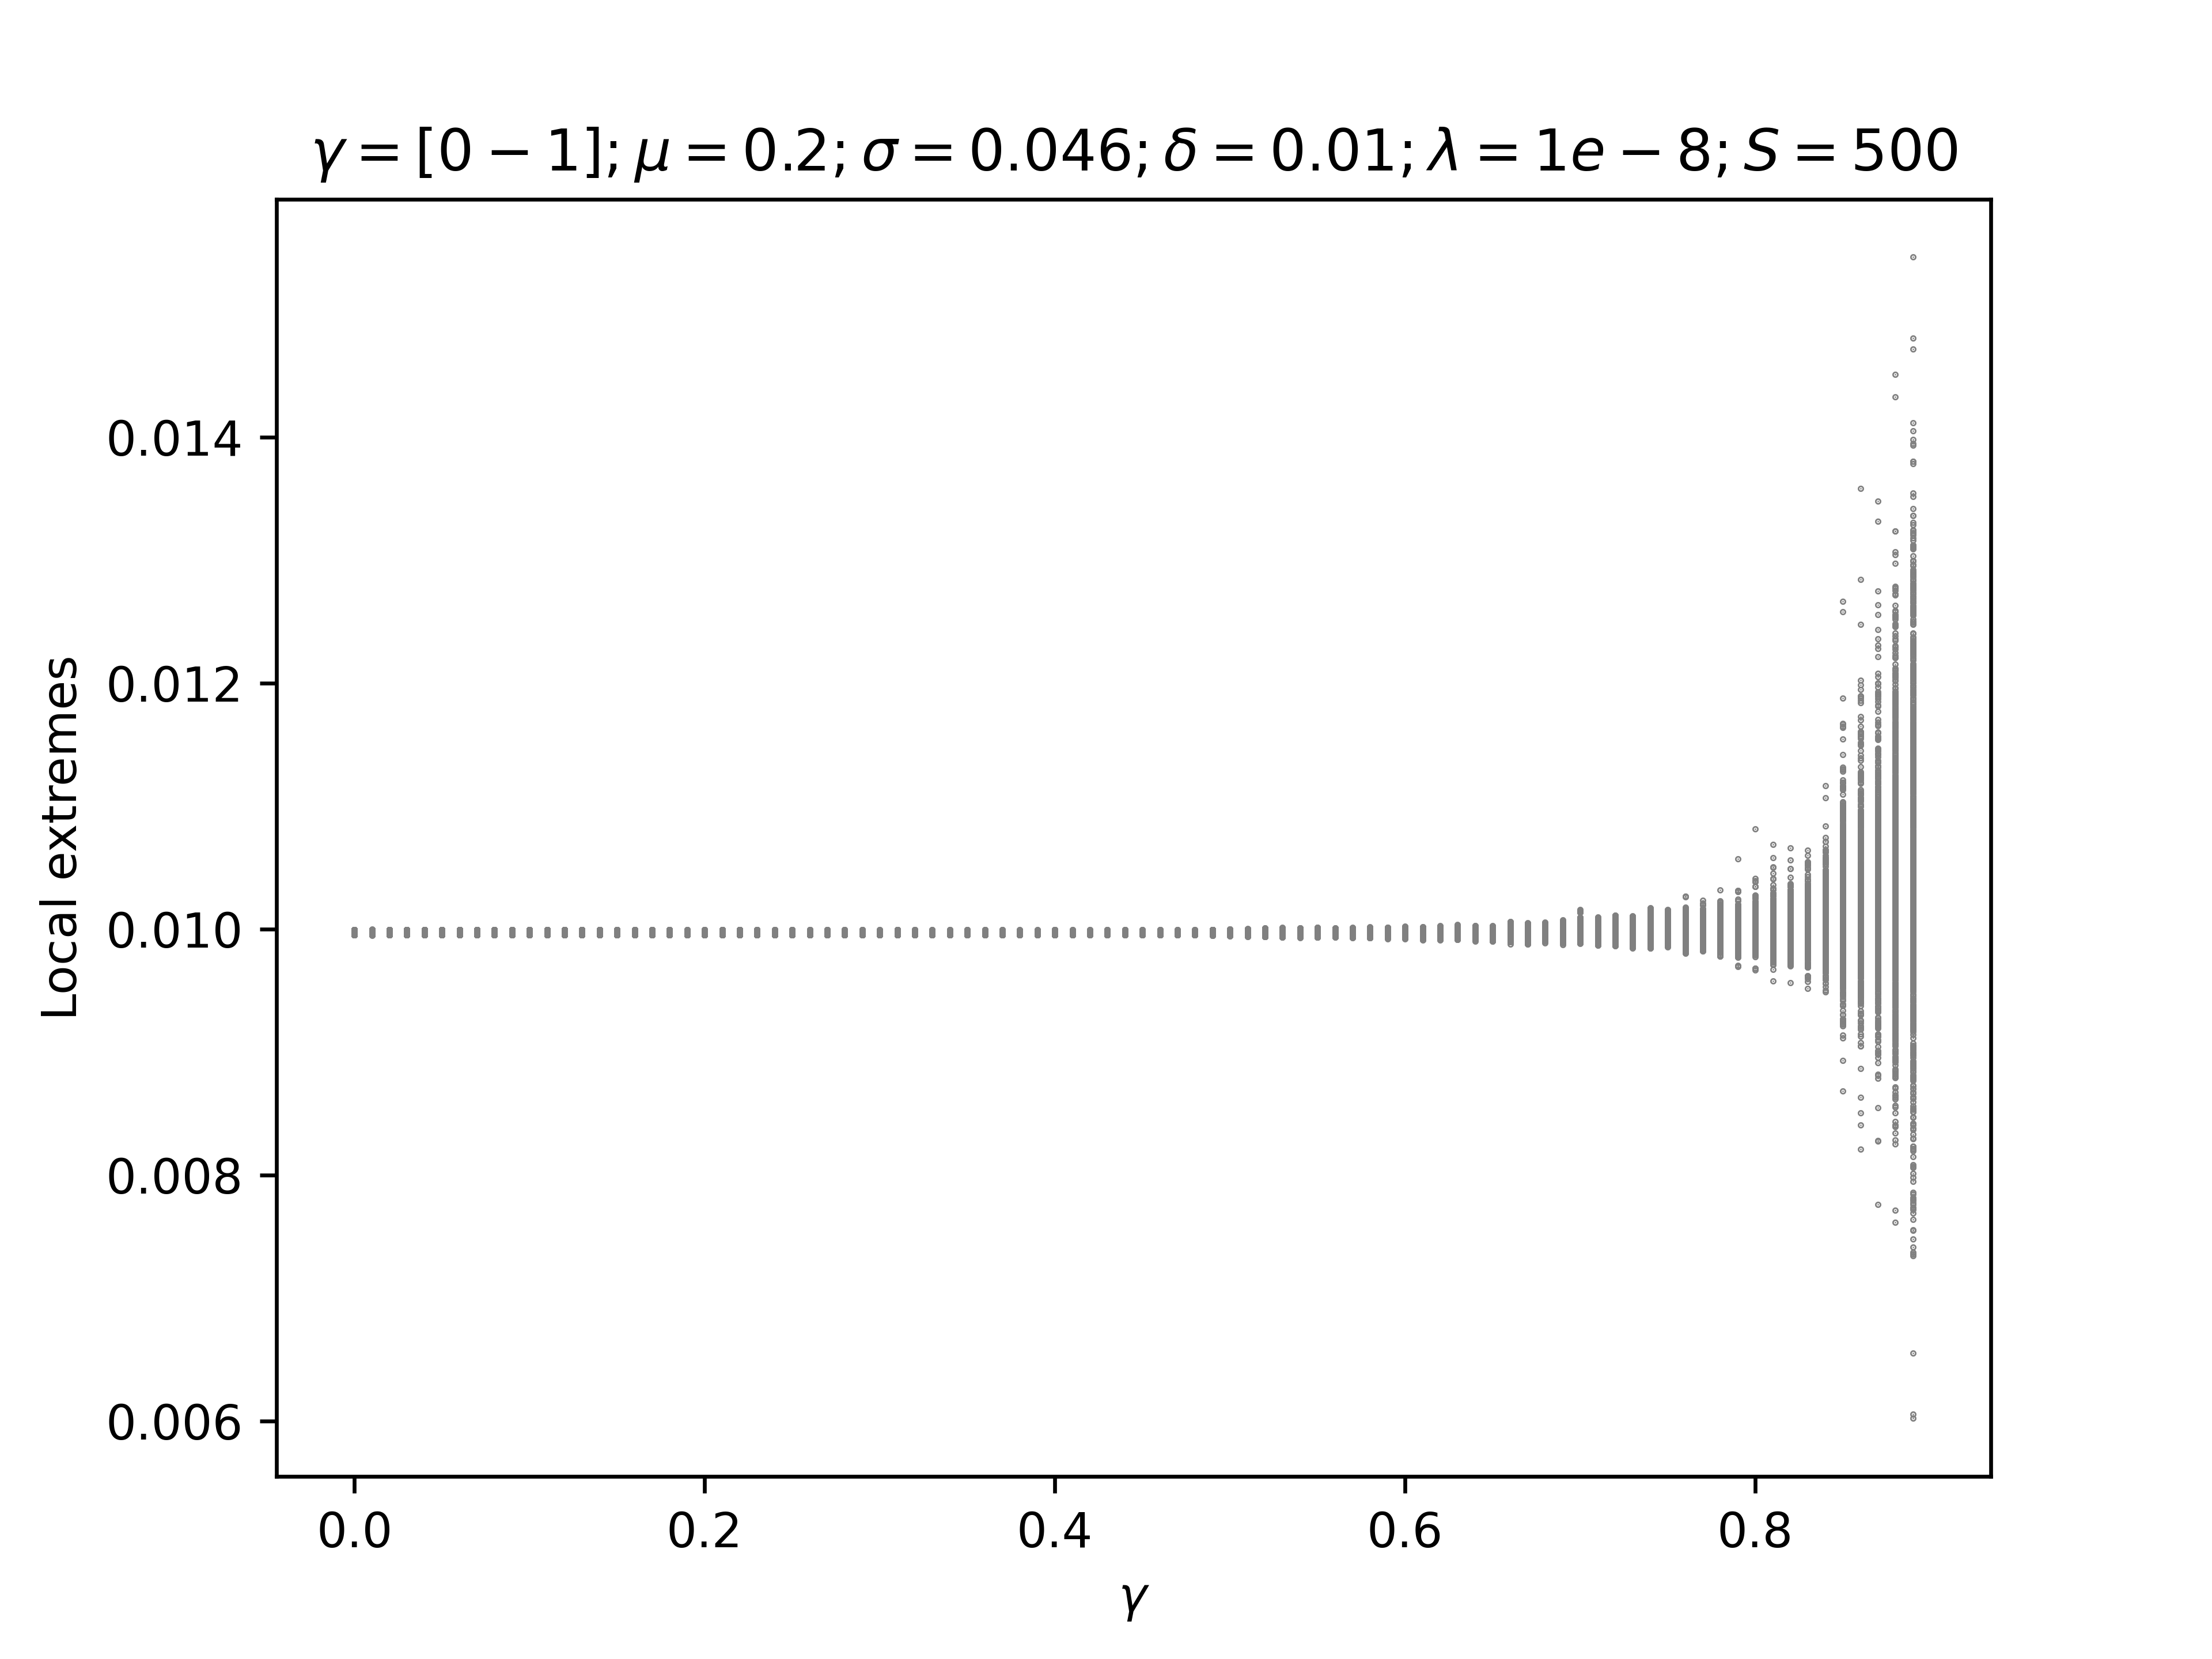
\includegraphics[width=\linewidth]{Bifurcation/BifurcationMeanGamma.png}
    \caption{Local extremes of the mean abundance of all species as a function of $\gamma$ varying from 0 to 0.89.}
\end{figure}

\begin{figure}[H]
    \centering
    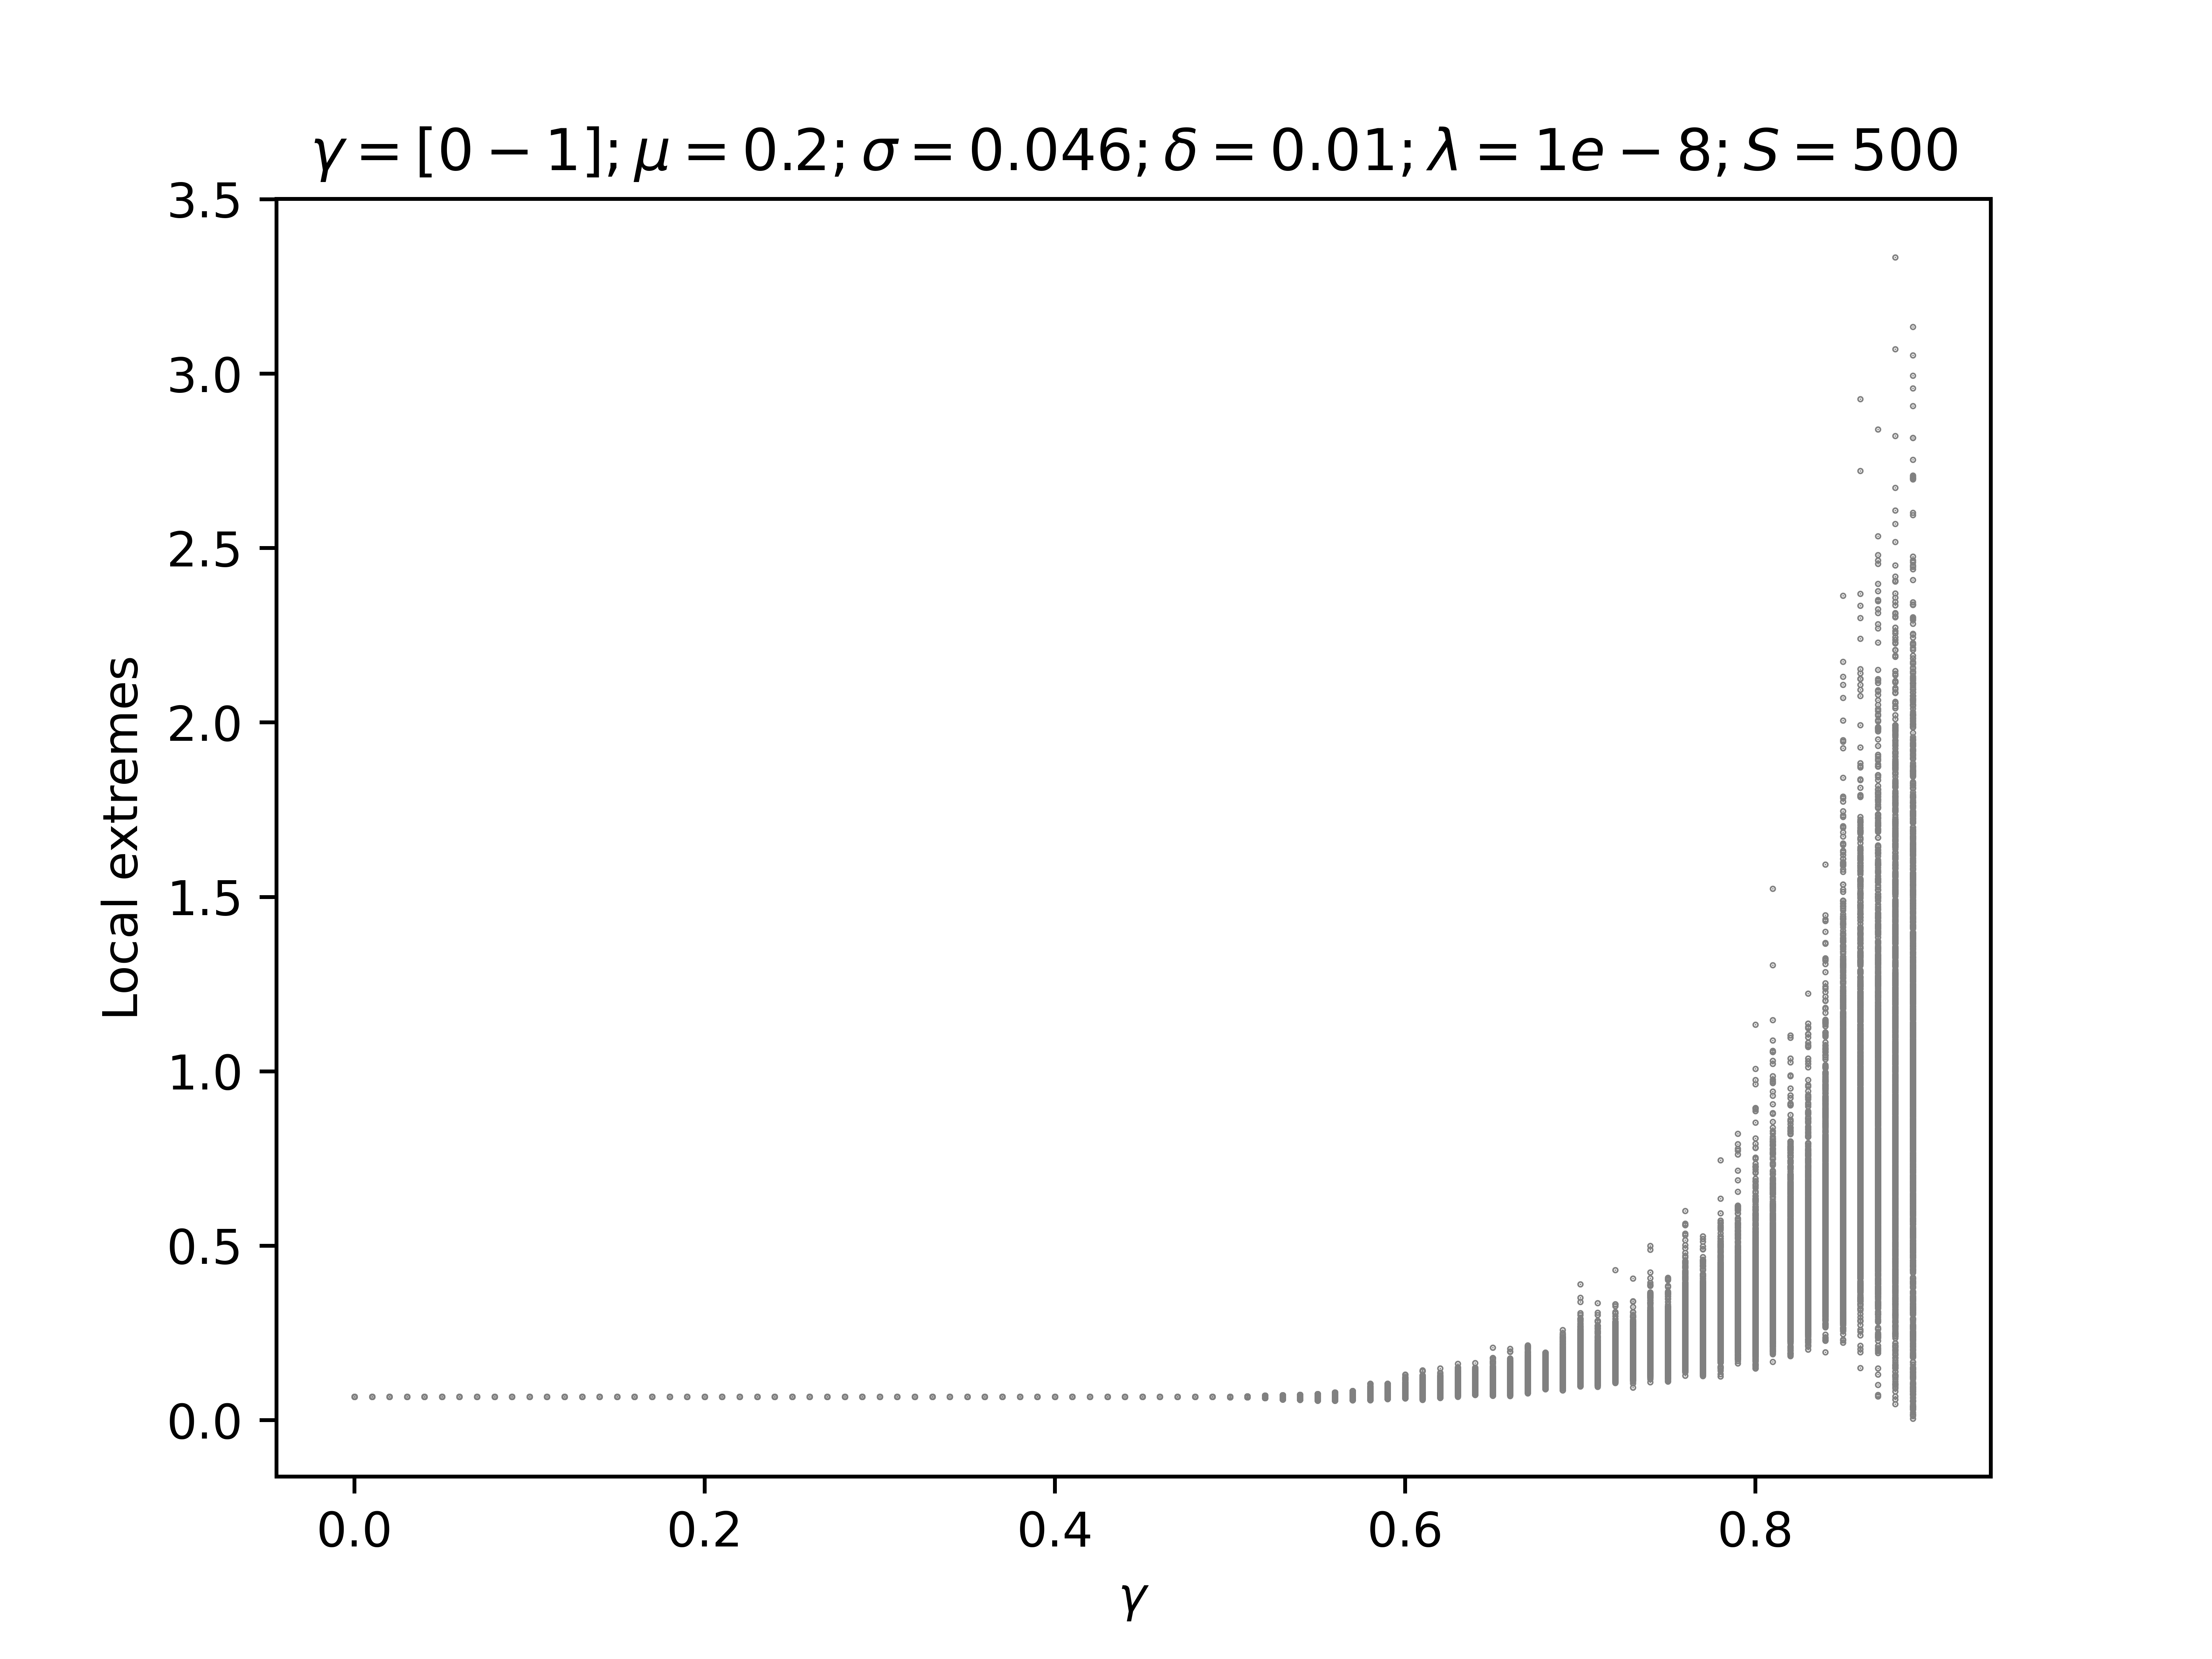
\includegraphics[width=\linewidth]{Bifurcation/BifurcationM1.png}
    \caption{Local extremes of the most abundant species as a function of $\gamma$ varying from 0 to 0.89.}
\end{figure}
\clearpage

\subparagraph{Varying $\delta$ from 0.001 to 0.022}

\begin{figure}[H]
    \centering
    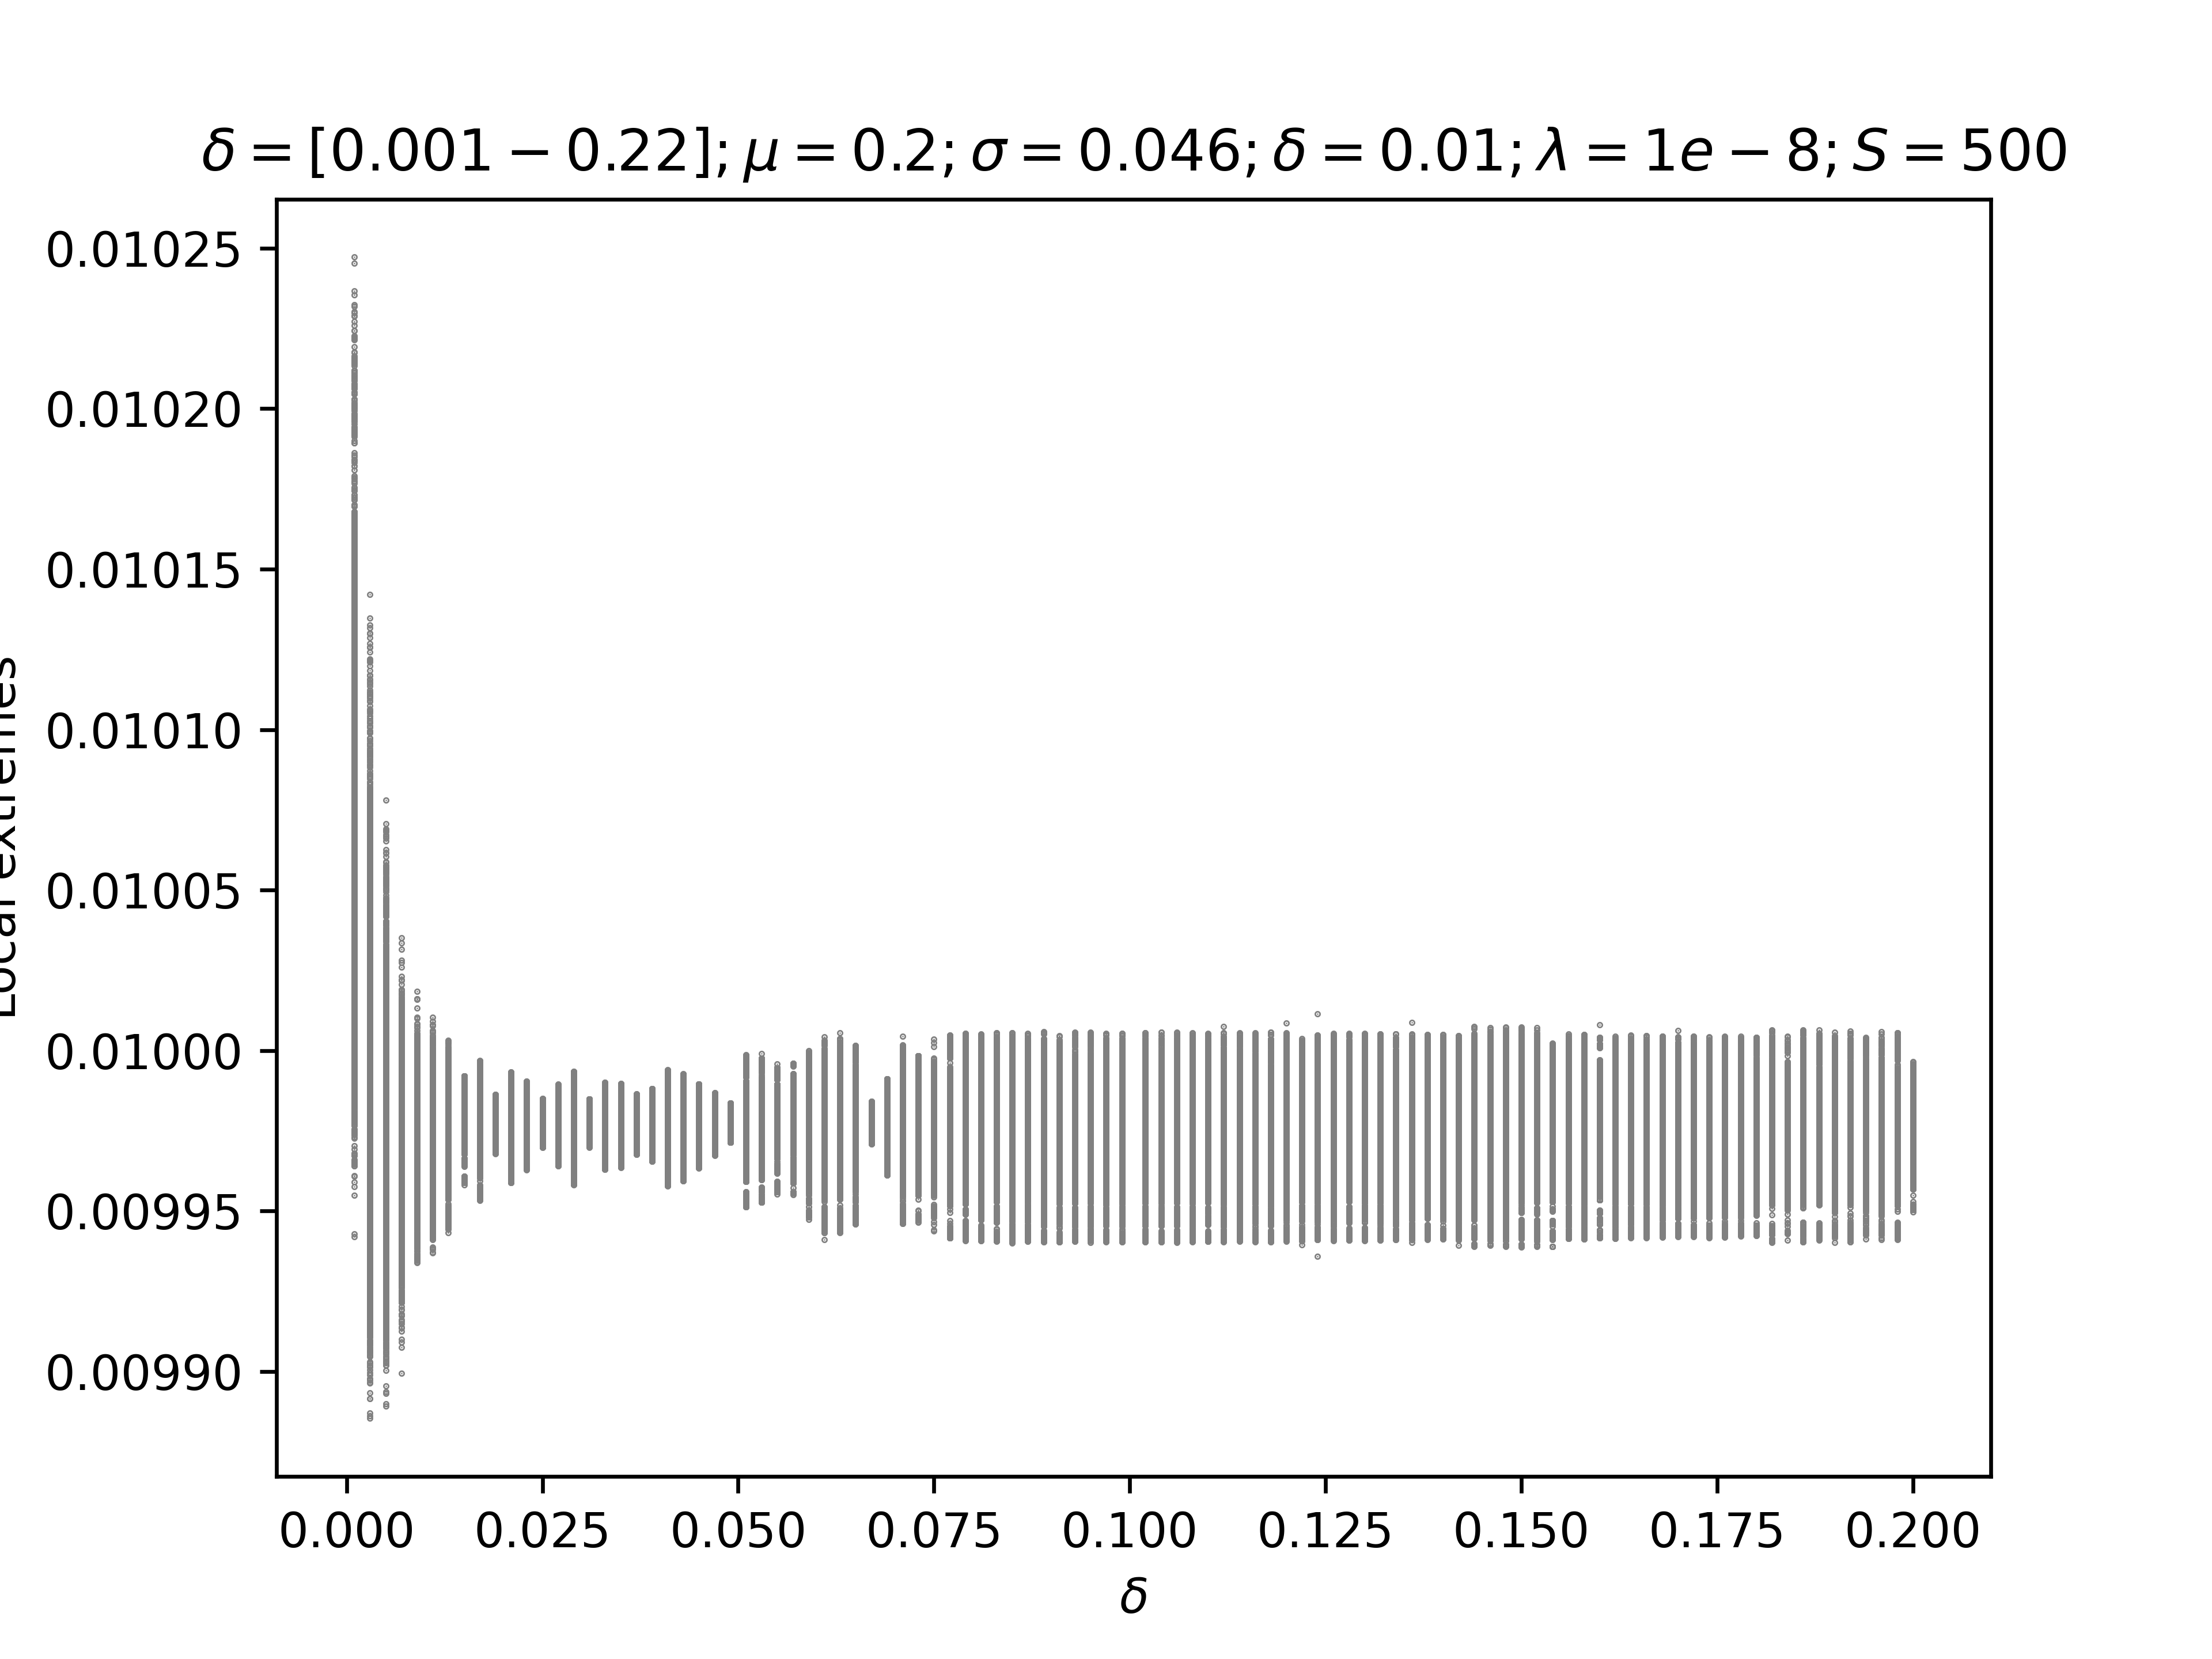
\includegraphics[width=\linewidth]{Bifurcation/BifurcationMeanDelta.png}
    \caption{Local extremes of the mean abundance of all species as a function of $\delta$ varying from 0.001 to 0.022.}
\end{figure}

\begin{figure}[H]
    \centering
    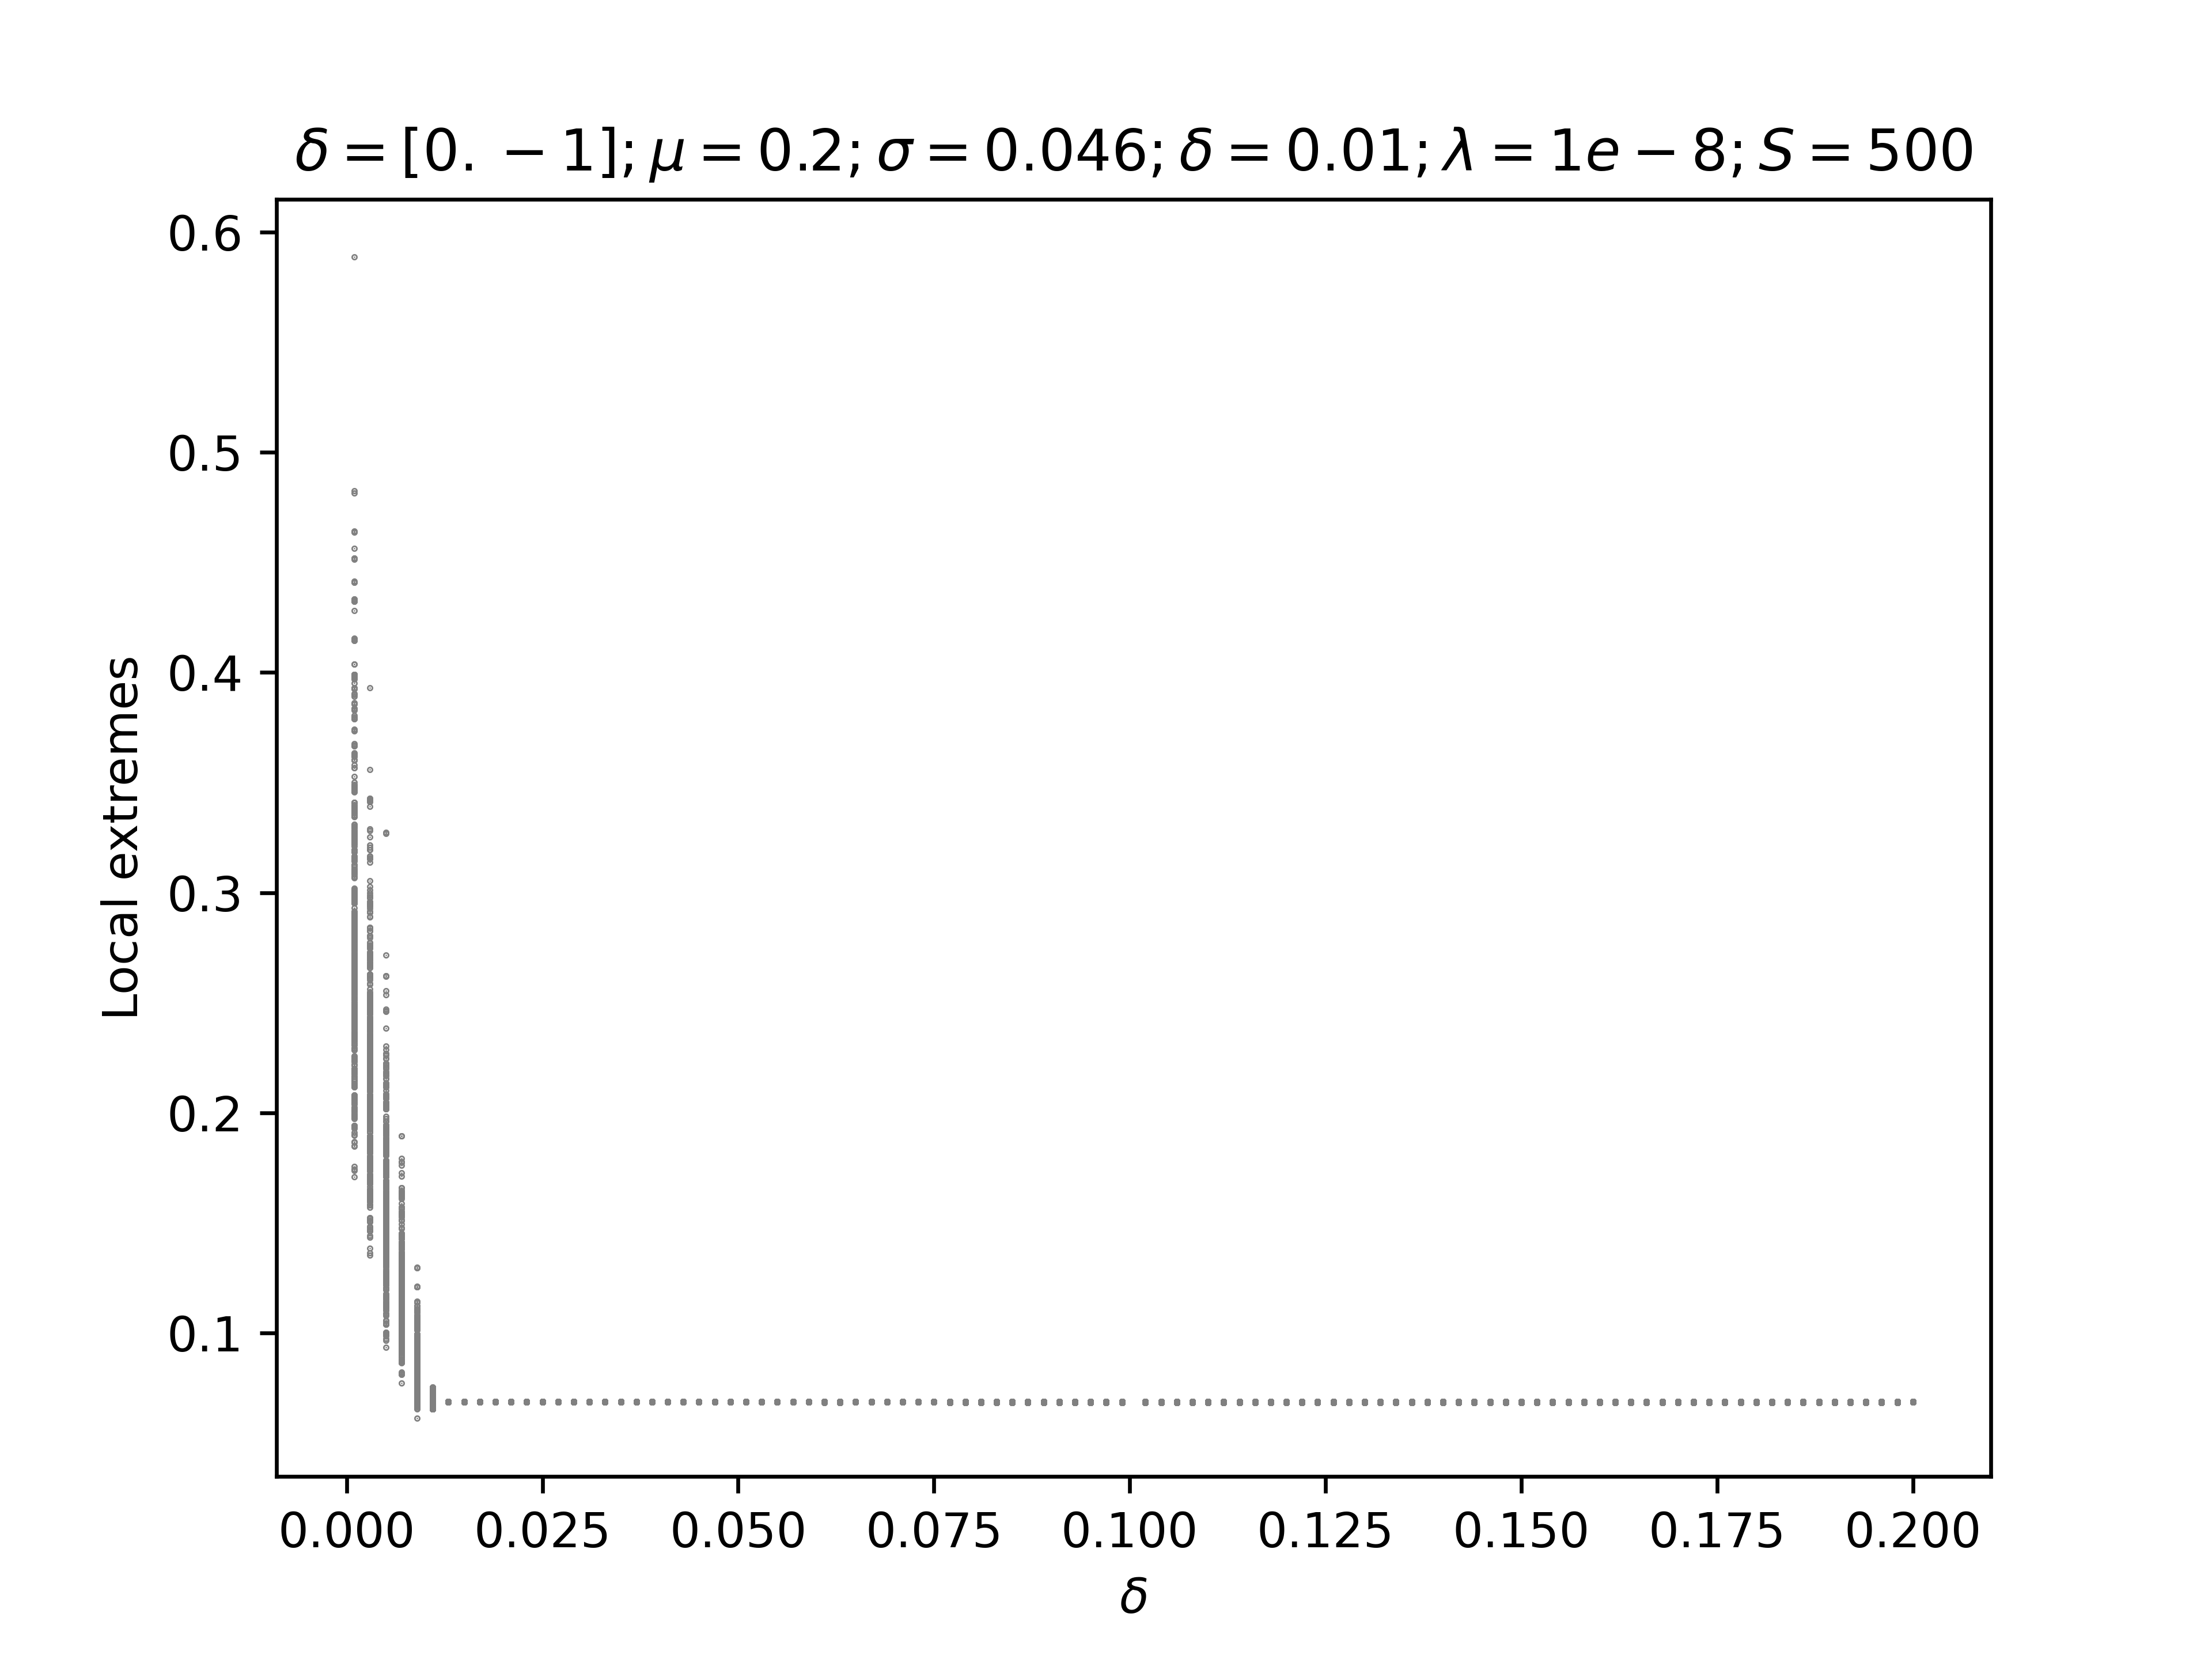
\includegraphics[width=\linewidth]{Bifurcation/BifurcationM1Delta.png}
    \caption{Local extremes of the most abundant species as a function of $\delta$ varying from 0.001 to 0.022.}
\end{figure}
\clearpage

\end{document}
